% !TeX program = xelatex
% !TEX TS-program = xelatex
% Compile with: xelatex final_report.tex (twice for TOC)
\documentclass[11pt,a4paper]{ctexart}
\usepackage{iftex}
\ifPDFTeX
  \PackageError{final_report}{請以 XeLaTeX 編譯本文件}{請改用 xelatex 指令或 latexmk 設定為 xelatex}
\fi

% Page and typography
\usepackage[a4paper,margin=1in]{geometry}
\usepackage{setspace}
\setstretch{1.2}
% Relax line-breaking a bit to avoid minor overfull boxes
\emergencystretch=2pt
\usepackage{hyperref}
\hypersetup{colorlinks=true, linkcolor=black, urlcolor=black, citecolor=black}
\usepackage{graphicx}
% Ensure images are included (not in draft) and set search paths
\setkeys{Gin}{draft=false}
\graphicspath{{./}{/Users/jesse/Documents/School Work/高等資料庫/cloud-infrastructure-analysis/Report/}}
\usepackage{booktabs}
\usepackage{array}
\usepackage{enumitem}
\usepackage{float}
\usepackage{subcaption}
\usepackage{tocloft}
% Tighten TOC spacing so last entry doesn't spill to next page
\setlength{\cftbeforesecskip}{2pt}
\setlength{\cftbeforesubsecskip}{1pt}
\setlength{\cftaftertoctitleskip}{8pt}

% Listings for Cypher and code
\usepackage{listings}
\usepackage{xcolor}
\definecolor{codebg}{RGB}{255,255,255}
\definecolor{codeframe}{RGB}{220,220,220}
\lstdefinelanguage{Cypher}{
  morekeywords={MATCH,RETURN,WHERE,AND,OR,NOT,WITH,CREATE,MERGE,DETACH,DELETE,SET,ON,EXISTS,UNWIND,OPTIONAL,AS,DISTINCT,TRUE,FALSE,NULL},
  sensitive=true,
  morestring=[b]",
  morecomment=[l]{//}
}
\lstset{
  language=Cypher,
  backgroundcolor=\color{codebg},
  basicstyle=\ttfamily\small,
  keywordstyle=\bfseries\color{black},
  commentstyle=\color{black},
  stringstyle=\color{black},
  frame=single,
  rulecolor=\color{black},
  frameround=tttt,
  breaklines=true,
  columns=fullflexible,
  tabsize=2,
  showstringspaces=false,
  keepspaces=true,
  numbers=left,
  numberstyle=\scriptsize\color{gray},
  xleftmargin=1em,
  framexleftmargin=1em
}

% Python code style
\lstdefinestyle{python}{
  language=Python,
  backgroundcolor=\color{codebg},
  basicstyle=\ttfamily\small,
  keywordstyle=\bfseries\color{blue},
  commentstyle=\color{green!60!black},
  stringstyle=\color{red},
  numberstyle=\tiny\color{gray},
  breaklines=true,
  captionpos=b,
  keepspaces=true,
  numbers=left,
  numbersep=5pt,
  showspaces=false,
  showstringspaces=false,
  showtabs=false,
  tabsize=2,
  frame=single,
  rulecolor=\color{codeframe}
}

% JSON code style
\lstdefinestyle{json}{
  language=Python,
  morecomment=[l]{//}, % 支援 // 註解
  backgroundcolor=\color{codebg},
  basicstyle=\ttfamily\small,
  keywordstyle=\bfseries\color{blue},
  commentstyle=\color{green!60!black},
  stringstyle=\color{red},
  numberstyle=\tiny\color{gray},
  breaklines=true,
  captionpos=b,
  keepspaces=true,
  numbers=left,
  numbersep=5pt,
  showspaces=false,
  showstringspaces=false,
  showtabs=false,
  tabsize=2,
  frame=single,
  rulecolor=\color{codeframe}
}

% Title info
\title{圖形資料庫最終報告\\Cloud Infrastructure Analysis Platform\\雲端基礎設施視覺化分析平台}
\author{課程:高等資料庫系統\\姓名:梁祐嘉\\學號:01157145\\班級:資工 4B\\日期:2025年10月23日}
\date{}

% Traditional Chinese names for lists and ToC
\ctexset{
  contentsname = 目錄,
  listfigurename = 圖目錄,
  listtablename = 表目錄
}
% Use English-style short label for figure captions
\renewcommand{\figurename}{fig}
% System font setup for better CJK and code coverage (macOS)
% Requires XeLaTeX; ctex loads fontspec under XeLaTeX
\setmainfont{Times New Roman}
\setsansfont{Helvetica}
\setmonofont{Menlo}
\setCJKmainfont{PingFang TC}
\setCJKsansfont{PingFang TC}
\setCJKmonofont{PingFang TC}

\begin{document}
\maketitle

% Make abstract title larger, keep body at normalsize
\renewcommand{\abstractname}{\large 摘要}
\begin{abstract}
\normalsize
本報告提出一套以 Neo4j 為核心的雲端基礎設施知識圖譜平台,旨在以圖形資料模型整合與分析專案在 AWS/GCP/Azure 等雲端環境中的複雜資源、關聯與依賴,並提供資安漏洞分析、故障衝擊分析與成本優化核心情境之查詢與分析。系統採用 Python 腳本透過雲端 API 擷取設定資料,轉換為節點與關係後匯入 Neo4j,以圖為中心進行視覺化與查詢。
\end{abstract}

\tableofcontents
\clearpage

\section{專案概述}

『Cloud Infrastructure Visualization Analysis Platform』雲端基礎設施視覺化分析平台。在現今的雲端環境,像是 AWS 這樣的平台,管理數百甚至數千個互相連接的資源 (Resources),例如 \texttt{EC2 instances}、\texttt{Databases}、\texttt{Firewalls} (\texttt{Security Groups})、\texttt{Load Balancers} 等,變得非常複雜。傳統的 List 或儀表板 Dashboard 很難呈現資源間的多層次(multi-hop)關聯,使得評估安全風險、分析故障影響範圍,或是找出可以節省成本的地方變得十分困難。我們的解決方案是利用 \texttt{Neo4j} 這個圖形資料庫 (Graph Database),將 infrastructure 的關係模型化,轉換成一個更直觀的、可深度查詢的圖譜,方便我們進行視覺化與分析。

\subsection{專案目標}
\begin{itemize}[leftmargin=1.5em]
\item \textbf{視覺化複雜基礎設施} - 將雲端資源轉換為易理解的圖形模型
\item \textbf{智能分析} - 自動識別安全風險、故障點和成本浪費
\item \textbf{即時監控} - 提供動態的基礎設施健康度評估
\item \textbf{決策支援} - 為基礎設施優化提供數據驅動的建議
\end{itemize}

\subsection{核心功能}

平台主要聚焦在於自動化分析三個領域:

\begin{enumerate}[leftmargin=1.5em]
\item \textbf{Security Vulnerability Analysis (資安漏洞分析):} 自動檢測暴露在公網的 High Risk 的服務(例如開放的 \texttt{SSH} 或 \texttt{RDP} ports)、過度寬鬆的防火牆規則 (\texttt{Security Group rules}),以及未加密的儲存資源 (\texttt{EBS volumes}) 等。

\item \textbf{Failure Impact Analysis (故障衝擊分析):} 識別 Infra 中的『關鍵節點』(Critical Nodes - 連接數多的資源)和『單點故障』(Single Points of Failure),分析潛在故障可能擴散的路徑。

\item \textbf{Cost Optimization Analysis (成本優化分析):} 找出未被使用的『孤兒資源』(Orphaned Resources),例如沒有掛載到任何 \texttt{EC2 instance} 的 \texttt{EBS volumes},或是未被使用的 \texttt{Security Groups},估算潛在的成本節省。
\end{enumerate}

\section{Neo4j 產品與服務}

\subsection{使用的 Neo4j 產品}
\begin{itemize}[leftmargin=1.5em]
\item \textbf{Neo4j Aura}: 雲端託管的 Neo4j 圖形資料庫服務
\item \textbf{Neo4j Browser}: 網頁介面查詢工具
\item \textbf{Cypher Query Language}: 圖形查詢語言
\item \textbf{Neo4j Python Driver}: 程式化連接工具
\item \textbf{Neo4j Dashboard}: 視覺化工具
\end{itemize}

\subsection{技術架構}
\begin{verbatim}
雲端 API (AWS) → 資料擷取層 → 資料轉換層 → Neo4j 圖形資料庫 → 分析引擎 → 視覺化層
     ↓              ↓              ↓              ↓              ↓           ↓
  Boto3 SDK     AWSExtractor   資料標準化     圖形模型化     Cypher 查詢   Dash 儀表板
\end{verbatim}

\section{原始資料格式與來源}

\subsection{資料格式}
\begin{itemize}[leftmargin=1.5em]
\item \textbf{格式}: JSON
\item \textbf{來源}: 模擬 AWS 資源資料 (Mock Data)
\item \textbf{結構}: 巢狀 JSON 物件,包含 EC2、VPC、Security Groups 等資源
\end{itemize}

\subsection{資料範例}

在 \texttt{VS Code Terminal} 中執行一個快速啟動腳本 (\texttt{quick\_start.sh})。這個腳本會幫我們設置好 \texttt{Python} 虛擬環境,檢查與 \texttt{Neo4j} 資料庫的連線,並載入我們預先準備好的模擬資料 (\texttt{mock data}) 到 \texttt{Neo4j} 中。

\begin{lstlisting}[language=bash, caption={快速啟動腳本}]
./scripts/quick_start.sh
\end{lstlisting}

Mock Data 載入完成。這些模擬資料是以 \texttt{JSON} 格式提供的,模擬真實 \texttt{AWS} 環境的資源配置。其中一筆 \texttt{EC2 Instance} 的資料:

\begin{lstlisting}[style=json, caption={EC2 Instance 資料範例}]
{
  "InstanceID": "i-4565ff31fc57641ab", // EC2 的唯一 ID (Unique ID)
  "Name": "recommendation-engine-staging-01", // 人工設定的名稱 (Name Tag)
  "State": { 
      "Name": "stopped" 
  }, // 目前狀態 (State)
  "InstanceType": "c5.xlarge", // 實例規格 (Instance Type)
  "SecurityGroups": [ // 它所屬的安全群組 (Security Groups)
    { 
        "GroupId": "sg-8c6c6e0e1847bd533", "GroupName": "elasticsearch-dev" 
    }
  ],
  "SubnetId": "subnet-1a56a26f43475ddf4", // 所在的子網路 ID (Subnet ID)
  "VpcId": "vpc-9218c5cf0d06f1bc3" // 所在的虛擬私有雲 ID (VPC ID)
}
\end{lstlisting}

這個 \texttt{JSON} 描述了 \texttt{EC2 Instance} \texttt{i-4565ff31fc57641ab} 的詳細資訊,包括它的狀態 (\texttt{stopped})、類型 (\texttt{c5.xlarge})、所屬的 \texttt{Security Groups} (\texttt{sg-8c6c6e0e1847bd533} 等)、所在的網路 (\texttt{SubnetId}, \texttt{VpcId}) 以及環境標籤 (\texttt{staging}) 等。我們的 \texttt{Python} 載入器 (\texttt{neo4j\_loader.py}) 會讀取這個 \texttt{JSON},並在 \texttt{Neo4j} 中創建對應的節點 (Nodes) 和關係 (Relationships)。

\section{圖形資料模型設計}

\subsection{核心節點(Nodes)}
\begin{itemize}[leftmargin=1.5em]
\item \texttt{:EC2Instance} - 屬性包含 \texttt{InstanceID}, \texttt{Name}, \texttt{State}, \texttt{PublicIP}。
\item \texttt{:SecurityGroup} - 屬性包含 \texttt{GroupID}, \texttt{GroupName}。
\item \texttt{:Rule} - 屬性包含 \texttt{Protocol}, \texttt{PortRange}, \texttt{SourceCIDR}。
\item \texttt{:VPC}、\texttt{:Subnet}、\texttt{:ELB}、\texttt{:S3Bucket}。
\end{itemize}

\subsection{核心關係(Relationships)}
\begin{itemize}[leftmargin=1.5em]
\item \texttt{(EC2Instance)-[:IS\_MEMBER\_OF]->(SecurityGroup)}
\item \texttt{(SecurityGroup)-[:HAS\_RULE]->(Rule)}
\item \texttt{(EC2Instance)-[:RESIDES\_IN]->(Subnet)},\texttt{(Subnet)-[:PART\_OF]->(VPC)}
\item \texttt{(ELB)-[:ROUTES\_TO]->(EC2Instance)}
\end{itemize}

\subsection{節點類型詳細說明}

本系統定義了以下核心節點類型,每個節點都包含特定的屬性來描述雲端資源的特徵:

\subsubsection{EC2Instance 節點}
\textbf{用途:} 代表 AWS EC2 虛擬機器實例
\begin{itemize}[leftmargin=1.5em]
\item \texttt{instanceid} - EC2 實例的唯一識別碼(如:i-1234567890abcdef0)
\item \texttt{name} - 實例的名稱標籤(如:web-server-01)
\item \texttt{state} - 實例狀態(running, stopped, terminated)
\item \texttt{instancetype} - 實例類型(t3.micro, c5.large 等)
\item \texttt{publicip} - 公有 IP 地址
\item \texttt{privateip} - 私有 IP 地址
\item \texttt{region} - AWS 區域(us-east-1, ap-southeast-1 等)
\item \texttt{launchtime} - 啟動時間
\item \texttt{tags} - 標籤資訊(JSON 格式)
\end{itemize}

\subsubsection{SecurityGroup 節點}
\textbf{用途:} 代表 AWS 安全群組(防火牆規則群組)
\begin{itemize}[leftmargin=1.5em]
\item \texttt{groupid} - 安全群組的唯一識別碼(如:sg-12345678)
\item \texttt{name} - 安全群組名稱
\item \texttt{description} - 群組描述
\item \texttt{vpcid} - 所屬 VPC 的識別碼
\item \texttt{region} - AWS 區域
\end{itemize}

\subsubsection{SecurityRule 節點}
\textbf{用途:} 代表安全群組中的具體規則
\begin{itemize}[leftmargin=1.5em]
\item \texttt{ruleid} - 規則的唯一識別碼
\item \texttt{protocol} - 協定類型(tcp, udp, icmp, all)
\item \texttt{portrange} - 連接埠範圍(22, 80-443, 0-65535)
\item \texttt{sourcecidr} - 來源 IP 範圍(0.0.0.0/0, 10.0.0.0/8)
\item \texttt{direction} - 流量方向(inbound, outbound)
\item \texttt{description} - 規則描述
\end{itemize}

\subsubsection{VPC 節點}
\textbf{用途:} 代表 AWS 虛擬私有雲
\begin{itemize}[leftmargin=1.5em]
\item \texttt{vpcid} - VPC 的唯一識別碼(如:vpc-12345678)
\item \texttt{name} - VPC 名稱標籤
\item \texttt{cidrblock} - CIDR 區塊(如:10.0.0.0/16)
\item \texttt{state} - VPC 狀態(available, pending)
\item \texttt{region} - AWS 區域
\item \texttt{isdefault} - 是否為預設 VPC
\end{itemize}

\subsubsection{Subnet 節點}
\textbf{用途:} 代表 VPC 中的子網路
\begin{itemize}[leftmargin=1.5em]
\item \texttt{subnetid} - 子網路的唯一識別碼(如:subnet-12345678)
\item \texttt{name} - 子網路名稱標籤
\item \texttt{cidrblock} - 子網路 CIDR 區塊(如:10.0.1.0/24)
\item \texttt{availabilityzone} - 可用區域(如:us-east-1a)
\item \texttt{state} - 子網路狀態
\item \texttt{vpcid} - 所屬 VPC 的識別碼
\end{itemize}

\subsubsection{EBSVolume 節點}
\textbf{用途:} 代表 AWS EBS 磁碟
\begin{itemize}[leftmargin=1.5em]
\item \texttt{volumeid} - 磁碟的唯一識別碼(如:vol-12345678)
\item \texttt{name} - 磁碟名稱標籤
\item \texttt{size} - 磁碟大小(GB)
\item \texttt{volumetype} - 磁碟類型(gp3, gp2, io1, st1, sc1)
\item \texttt{state} - 磁碟狀態(available, in-use, creating)
\item \texttt{encrypted} - 是否加密(true/false)
\item \texttt{region} - AWS 區域
\item \texttt{creationdate} - 建立日期
\end{itemize}

\subsubsection{S3Bucket 節點}
\textbf{用途:} 代表 AWS S3 儲存桶
\begin{itemize}[leftmargin=1.5em]
\item \texttt{bucketname} - 儲存桶名稱
\item \texttt{region} - AWS 區域
\item \texttt{creationdate} - 建立日期
\item \texttt{versioning} - 版本控制狀態
\item \texttt{encryption} - 加密設定
\item \texttt{publicaccess} - 公開存取設定
\end{itemize}

\subsection{關係類型詳細說明}

本系統定義了以下核心關係類型,用於描述雲端資源之間的連接和依賴關係:

\subsubsection{IS\_MEMBER\_OF 關係}
\textbf{用途:} 表示 EC2 實例屬於某個安全群組
\begin{itemize}[leftmargin=1.5em]
\item \textbf{方向:} \texttt{(EC2Instance)-[:IS\_MEMBER\_OF]->(SecurityGroup)}
\item \textbf{意義:} EC2 實例受到該安全群組的防火牆規則保護
\item \textbf{屬性:} 通常不包含額外屬性,關係本身即表示成員資格
\item \textbf{查詢用途:} 用於分析哪些實例受到特定安全群組保護,或找出未受保護的實例
\end{itemize}

\subsubsection{HAS\_RULE 關係}
\textbf{用途:} 表示安全群組包含特定的安全規則
\begin{itemize}[leftmargin=1.5em]
\item \textbf{方向:} \texttt{(SecurityGroup)-[:HAS\_RULE]->(SecurityRule)}
\item \textbf{意義:} 安全群組定義了具體的網路存取規則
\item \textbf{屬性:} 可能包含規則優先級或啟用狀態
\item \textbf{查詢用途:} 用於分析安全群組的規則配置,識別過度寬鬆的規則
\end{itemize}

\subsubsection{LOCATED\_IN 關係}
\textbf{用途:} 表示資源位於特定的網路位置
\begin{itemize}[leftmargin=1.5em]
\item \textbf{方向:} \texttt{(EC2Instance)-[:LOCATED\_IN]->(Subnet)},\texttt{(Subnet)-[:LOCATED\_IN]->(VPC)}
\item \textbf{意義:} 描述資源的網路層級位置關係
\item \textbf{屬性:} 可能包含 IP 地址分配資訊
\item \textbf{查詢用途:} 用於分析網路拓撲,識別跨可用區域的冗餘性
\end{itemize}

\subsubsection{ATTACHES\_TO 關係}
\textbf{用途:} 表示 EBS 磁碟掛載到 EC2 實例
\begin{itemize}[leftmargin=1.5em]
\item \textbf{方向:} \texttt{(EBSVolume)-[:ATTACHES\_TO]->(EC2Instance)}
\item \textbf{意義:} EBS 磁碟被掛載到特定的 EC2 實例上
\item \textbf{屬性:} 可能包含掛載點和掛載狀態
\item \textbf{查詢用途:} 用於識別孤兒磁碟(未掛載的磁碟)和磁碟使用情況
\end{itemize}


\section{核心分析功能與範例查詢}\label{sec:analysis}
本系統聚焦三大分析場景:資安漏洞分析、故障衝擊分析與成本優化分析。以下提供代表性 Cypher 查詢。

\subsection{資安漏洞分析(Security Vulnerability Analysis)}
\textbf{目標} - 找出所有暴露於公網且開啟高風險連接埠(如 SSH:22, RDP:3389)的主機。

\begin{lstlisting}[language=Cypher,caption={尋找允許 0.0.0.0/0 存取 22 埠之主機}]
// 找出所有允許從任何 IP (0.0.0.0/0) 存取 22 號連接埠的主機
MATCH (instance:EC2Instance)-[:IS_MEMBER_OF]->(sg:SecurityGroup),
      (sg)-[:HAS_RULE]->(rule:Rule)
WHERE rule.SourceCIDR = '0.0.0.0/0' AND rule.PortRange CONTAINS '22'
RETURN instance.Name, instance.InstanceID, instance.PublicIP
\end{lstlisting}

\subsection{故障衝擊分析(Failure Impact Analysis)}
\textbf{目標} - 由特定資料庫(如 \texttt{db-main})出發,找出依賴該資料庫的應用主機。

\begin{lstlisting}[language=Cypher,caption={由資料庫反向追蹤依賴它的應用主機}]
// 假設存在 (EC2)-[:CONNECTS_TO]->(Database) 的關係
MATCH (db:Database {Name: 'db-main'})<-[:CONNECTS_TO*1..5]-(app:EC2Instance)
RETURN DISTINCT app.Name AS AffectedApplication
\end{lstlisting}

\subsection{成本優化分析(Cost Optimization Analysis)}
\textbf{目標} - 找出帳號中的「孤兒硬碟」(Orphaned EBS Volumes)。

\begin{lstlisting}[language=Cypher,caption={找出未連接至任何 EC2 的 EBS 磁碟}]
MATCH (vol:EBSVolume)
WHERE NOT (vol)-[:ATTACHES_TO]->(:EC2Instance)
RETURN vol.VolumeID, vol.Size, vol.CreationDate
\end{lstlisting}

\subsection{詳細查詢語句解析}

本節提供完整的 Cypher 查詢語句解析,涵蓋安全性、成本和可靠性分析的核心查詢。

\subsubsection{安全性分析查詢}

\textbf{1. 未加密的 EBS 磁碟檢測}

\begin{lstlisting}[language=Cypher,caption={找出未加密的 EBS 磁碟}]
MATCH (v:EBSVolume) 
WHERE v.encrypted = false
RETURN v.volumeid AS VolumeID, v.region AS Region, v.state AS State, v.size AS SizeGB
\end{lstlisting}

\textbf{查詢解析:}
\begin{itemize}[leftmargin=1.5em]
\item \texttt{MATCH (v:EBSVolume)} - 尋找圖形資料庫中所有標記為 \texttt{EBSVolume} 的節點
\item \texttt{WHERE v.encrypted = false} - 篩選出 \texttt{encrypted} 屬性為 \texttt{false} 的磁碟
\item \texttt{RETURN ...} - 回傳未加密磁碟的詳細資訊
\item \textbf{用途} - 找出不符合加密安全規範的 EBS 磁碟
\end{itemize}

\textbf{2. 過度寬鬆的安全群組檢測}

\begin{lstlisting}[language=Cypher,caption={找出過度寬鬆的安全性群組}]
MATCH (sg:SecurityGroup)-[:HAS_RULE]->(sr:SecurityRule) 
WHERE sr.sourcecidr = '0.0.0.0/0'
AND sr.direction = 'inbound'
RETURN sg.groupid AS SecurityGroupID, sg.name AS SecurityGroupName, 
       sr.protocol AS Protocol, sr.portrange AS PortRange, sr.description AS RuleDescription
\end{lstlisting}

\textbf{查詢解析:}
\begin{itemize}[leftmargin=1.5em]
\item \texttt{MATCH (sg:SecurityGroup)-[:HAS\_RULE]->(sr:SecurityRule)} - 尋找安全群組及其規則的關聯
\item \texttt{WHERE sr.sourcecidr = '0.0.0.0/0' AND sr.direction = 'inbound'} - 篩選允許任何 IP 存取的傳入規則
\item \textbf{用途} - 這是一個重大的安全檢查,用於找出所有向全世界開放的服務埠
\end{itemize}

\subsubsection{成本優化分析查詢}

\textbf{3. 未掛載的 EBS 磁碟檢測}

\begin{lstlisting}[language=Cypher,caption={找出未掛載的 EBS 磁碟}]
MATCH (v:EBSVolume) 
WHERE NOT (v)--(:EC2Instance) 
RETURN v.volumeid AS VolumeID, v.region AS Region, v.state AS State, v.size AS SizeGB
\end{lstlisting}

\textbf{查詢解析:}
\begin{itemize}[leftmargin=1.5em]
\item \texttt{MATCH (v:EBSVolume)} - 尋找所有 EBS 磁碟節點
\item \texttt{WHERE NOT (v)--(:EC2Instance)} - 篩選沒有關聯到任何 EC2 實例的磁碟
\item \textbf{用途} - 找出未被使用的 EBS 磁碟,這些磁碟仍會產生儲存費用
\end{itemize}

\textbf{4. 未使用的安全群組檢測}

\begin{lstlisting}[language=Cypher,caption={找出未使用的安全性群組}]
MATCH (sg:SecurityGroup) 
WHERE NOT (:EC2Instance)-->(sg) 
AND EXISTS((sg)-[:HAS_RULE]->(:SecurityRule)) 
RETURN sg.groupid AS SecurityGroupID, sg.name AS SecurityGroupName, 
       sg.vpcid AS VPCID, sg.region AS Region
\end{lstlisting}

\textbf{查詢解析:}
\begin{itemize}[leftmargin=1.5em]
\item \texttt{WHERE NOT (:EC2Instance)-->(sg)} - 篩選沒有被任何 EC2 實例使用的安全群組
\item \texttt{AND EXISTS((sg)-[:HAS\_RULE]->(:SecurityRule))} - 確保這些群組確實定義了規則
\item \textbf{用途} - 清理舊的或已棄用的安全群組,簡化網路管理
\end{itemize}

\textbf{5. 已停止的 EC2 實例檢測}

\begin{lstlisting}[language=Cypher,caption={找出已停止的 EC2 執行個體}]
MATCH (i:EC2Instance) 
WHERE i.state = 'stopped'
RETURN i.instanceid AS InstanceID, i.name AS InstanceName, i.region AS Region, 
       i.instancetype AS InstanceType, i.launchtime AS LaunchTime
\end{lstlisting}

\textbf{查詢解析:}
\begin{itemize}[leftmargin=1.5em]
\item \texttt{WHERE i.state = 'stopped'} - 篩選狀態為 \texttt{stopped} 的實例
\item \textbf{用途} - 找出長時間停止的 EC2 實例,雖然停止的 EC2 不會收取運算費用,但掛載的 EBS 磁碟仍會收費
\end{itemize}

\subsubsection{故障衝擊分析查詢}

\textbf{6. 關鍵節點識別}

\begin{lstlisting}[language=Cypher,caption={找出關鍵節點}]
MATCH (n)
WITH n, COUNT { (n)--() } as connection_count
WHERE connection_count > 2
RETURN labels(n)[0] AS NodeType,
CASE
WHEN labels(n)[0] = 'EC2Instance' THEN n.name
WHEN labels(n)[0] = 'SecurityGroup' THEN n.name
WHEN labels(n)[0] = 'VPC' THEN n.vpcid
WHEN labels(n)[0] = 'Subnet' THEN n.subnetid
ELSE n.id
END AS NodeName,
connection_count AS ConnectionCount
ORDER BY ConnectionCount DESC
LIMIT 10
\end{lstlisting}

\textbf{查詢解析:}
\begin{itemize}[leftmargin=1.5em]
\item \texttt{MATCH (n)} - 匹配圖中的所有節點
\item \texttt{COUNT \{ (n)--() \} as connection\_count} - 計算每個節點的連接數
\item \texttt{WHERE connection\_count > 2} - 篩選連接數大於 2 的節點
\item \textbf{用途} - 找出圖中連接最緊密的關鍵節點,這些節點一旦發生故障,影響範圍可能最廣
\end{itemize}

\textbf{7. 單點故障檢測}

\begin{lstlisting}[language=Cypher,caption={找出單點故障}]
MATCH (n)
WITH n, COUNT { (n)--() } as connection_count
WHERE connection_count = 1
RETURN labels(n)[0] AS NodeType,
CASE
WHEN labels(n)[0] = 'EC2Instance' THEN n.name
WHEN labels(n)[0] = 'SecurityGroup' THEN n.name
WHEN labels(n)[0] = 'EBSVolume' THEN n.volumeid
ELSE n.id
END AS NodeName,
connection_count AS ConnectionCount
ORDER BY NodeType, NodeName
LIMIT 15
\end{lstlisting}

\textbf{查詢解析:}
\begin{itemize}[leftmargin=1.5em]
\item \texttt{WHERE connection\_count = 1} - 篩選連接數剛好等於 1 的節點
\item \textbf{用途} - 找出潛在的單點故障,這些節點位於圖形的末端,如果唯一連接失效就會被隔離
\end{itemize}

\textbf{8. 網路冗餘性分析}

\begin{lstlisting}[language=Cypher,caption={網路冗餘性分析}]
MATCH (vpc:VPC)
OPTIONAL MATCH (subnet:Subnet)-[:LOCATED_IN]->(vpc)
OPTIONAL MATCH (instance:EC2Instance)-[:LOCATED_IN]->(subnet)
WITH vpc, 
collect(DISTINCT subnet) as subnets,
collect(DISTINCT instance) as instances
RETURN
vpc.vpcid as VpcId,
size(subnets) as SubnetCount,
size(instances) as InstanceCount,
[subnet in subnets | {
id: subnet.subnetid,
az: subnet.availabilityzone,
cidr: subnet.cidrblock,
instance_count: COUNT { (instance:EC2Instance)-[:LOCATED_IN]->(subnet) }
}] as subnet_details
ORDER BY InstanceCount DESC
\end{lstlisting}

\textbf{查詢解析:}
\begin{itemize}[leftmargin=1.5em]
\item \texttt{OPTIONAL MATCH} - 使用選擇性匹配來找出 VPC 中的子網路和實例
\item \texttt{collect(DISTINCT ...)} - 收集每個 VPC 下的所有子網路和實例
\item \textbf{用途} - 全面分析每個 VPC 的資源分佈,檢查跨可用區域的冗餘性
\end{itemize}

\textbf{9. 一般圖形探索}

\begin{lstlisting}[language=Cypher,caption={一般圖形探索}]
MATCH (a)-[r]-(b) 
WHERE type(r) IN ['IS_MEMBER_OF', 'LOCATED_IN', 'ATTACHES_TO', 'HAS_RULE'] 
RETURN a, r, b 
LIMIT 200
\end{lstlisting}

\textbf{查詢解析:}
\begin{itemize}[leftmargin=1.5em]
\item \texttt{MATCH (a)-[r]-(b)} - 匹配任意兩個節點之間的關聯
\item \texttt{WHERE type(r) IN [...]} - 篩選核心的關聯類型
\item \textbf{用途} - 探索性查詢,用於快速了解圖形中的主要結構和連接方式
\end{itemize}

\section{實作要點}
\subsection{擷取與載入}
\begin{itemize}[leftmargin=1.5em]
\item \textbf{擷取頻率與版本控管} - 定期擷取 JSON 並保留版本,以支援變更比對與回溯。
\item \textbf{ID 去重與關聯完整性} - 以雲端資源原生 ID 作為主鍵,避免重覆匯入;匯入順序先節點後關係。
\item \textbf{安全性} - 妥善保護 API 金鑰,避免將敏感設定納入版本庫。
\end{itemize}

\subsection{查詢效能}
\begin{itemize}[leftmargin=1.5em]
\item 針對高選擇性屬性(如 \texttt{InstanceID}, \texttt{GroupID})建立索引或唯一性約束。
\item 對常見路徑查詢調整模式與方向性,減少掃描範圍。
\end{itemize}

\section{Neo4j 圖形資料庫的優勢}

\begin{enumerate}[leftmargin=1.5em]
\item \textbf{直觀呈現 (Intuitive Visualization):} 將抽象的雲端架構以節點和關係視覺化,使複雜的基礎設施關係一目了然。

\item \textbf{深度分析 (Deep Analysis):} 使用 \texttt{Cypher} 查詢語言可以輕鬆遍歷多層關係,執行複雜分析,發現傳統資料庫難以查詢的多跳連接。

\item \textbf{自動化檢測 (Automated Detection):} 腳本化的分析流程能自動找出潛在的安全、故障和成本問題,大幅提升運維效率。

\item \textbf{模組化架構 (Modular Architecture):} 系統設計參考了 \texttt{Cartography} 框架,易於擴展,未來可以加入對 \texttt{GCP}、\texttt{Azure} 等其他雲平台的支持,或增加更多自定義的分析規則。
\end{enumerate}

分析結果顯示,即便是模擬數據,我們也能識別出數十個有價值的洞見,證明了這個方法的有效性。

\section{結論}

\subsection{專案成果}

本專案成功實現了基於 Neo4j 圖形資料庫的雲端基礎設施分析平台,具備以下特色:

\begin{enumerate}[leftmargin=1.5em]
\item \textbf{直觀的視覺化}: 將複雜的雲端架構轉換為易於理解的圖形結構
\item \textbf{深度分析能力}: 使用 Cypher 查詢語言進行多層次關係分析
\item \textbf{自動化檢測}: 實現三大核心功能的自動化分析
\item \textbf{模組化設計}: 易於擴展和維護的架構設計
\end{enumerate}

\subsection{技術價值}

總結來說,這個基於 \texttt{Neo4j} 的平台成功地將複雜的雲端基礎設施轉化為一個動態的、可分析的知識圖譜 (Knowledge Graph)。它不僅僅是一個監控工具,更是一個能提供深度洞察和具體優化建議的決策支援系統。這充分展現了圖形資料庫在現代 \texttt{IT Operations} 和 \texttt{Cloud Management} 領域的強大應用潛力。

\begin{itemize}[leftmargin=1.5em]
\item \textbf{圖形資料庫優勢}: 展現了圖形資料庫在複雜關係分析中的優勢
\item \textbf{實用性}: 解決了實際的雲端管理問題
\item \textbf{可擴展性}: 為未來功能擴展奠定了良好基礎
\end{itemize}

\subsection{未來發展}

\begin{itemize}[leftmargin=1.5em]
\item \textbf{多雲支援}: 擴展至 GCP、Azure 等其他雲平台
\item \textbf{即時監控}: 實現即時資料更新和分析
\item \textbf{機器學習}: 整合 AI 技術進行智能分析
\item \textbf{視覺化增強}: 提供更豐富的圖形展示功能
\end{itemize}

\clearpage
\section{系統架構與儀表板工作原理}

\subsection{整體系統架構}

本系統採用模組化架構設計,主要組件包括:

\begin{enumerate}[leftmargin=1.5em]
\item \textbf{資料擷取層} - 從 AWS API 或模擬資料中擷取雲端資源資訊
\item \textbf{資料轉換層} - 將原始資料轉換為圖形資料模型
\item \textbf{Neo4j 圖形資料庫} - 儲存節點和關係,支援複雜查詢
\item \textbf{分析引擎} - 執行安全性、故障衝擊和成本優化分析
\item \textbf{視覺化儀表板} - 提供互動式 Web 介面展示分析結果
\end{enumerate}

\subsection{系統連接流程}

\begin{verbatim}
雲端 API (AWS) → 資料擷取層 → 資料轉換層 → Neo4j 圖形資料庫 → 分析引擎 → 視覺化層
     ↓              ↓              ↓              ↓              ↓           ↓
  Boto3 SDK     AWSExtractor   資料標準化     圖形模型化     Cypher 查詢   Flask 儀表板
\end{verbatim}

\subsection{儀表板工作原理}

\subsubsection{Flask 儀表板架構}

系統使用 \texttt{SimpleDashboard} 類別提供基於 Flask 的輕量級 Web 儀表板:

\begin{itemize}[leftmargin=1.5em]
\item \textbf{資料載入} - 從 JSON 分析結果文件載入資料
\item \textbf{API 端點} - 提供 RESTful API 供前端調用
\item \textbf{圖形視覺化} - 整合 \texttt{vis-network} 進行互動式圖形展示
\item \textbf{即時分析} - 支援動態查詢和結果更新
\end{itemize}

\subsubsection{核心 API 端點}

\begin{lstlisting}[language=Python,caption={儀表板 API 端點}]
@app.route('/api/data')      # 獲取所有分析數據
@app.route('/api/security')  # 獲取安全分析結果
@app.route('/api/failure')   # 獲取故障衝擊分析結果
@app.route('/api/cost')     # 獲取成本優化分析結果
\end{lstlisting}

\subsubsection{前端視覺化技術}

\begin{itemize}[leftmargin=1.5em]
\item \textbf{vis-network} - 互動式圖形網路視覺化
\item \textbf{Chart.js} - 統計圖表展示
\item \textbf{FontAwesome} - 圖標系統
\item \textbf{響應式設計} - 支援多種螢幕尺寸
\end{itemize}

\subsection{系統截圖展示}

\begin{figure}[H]
\centering
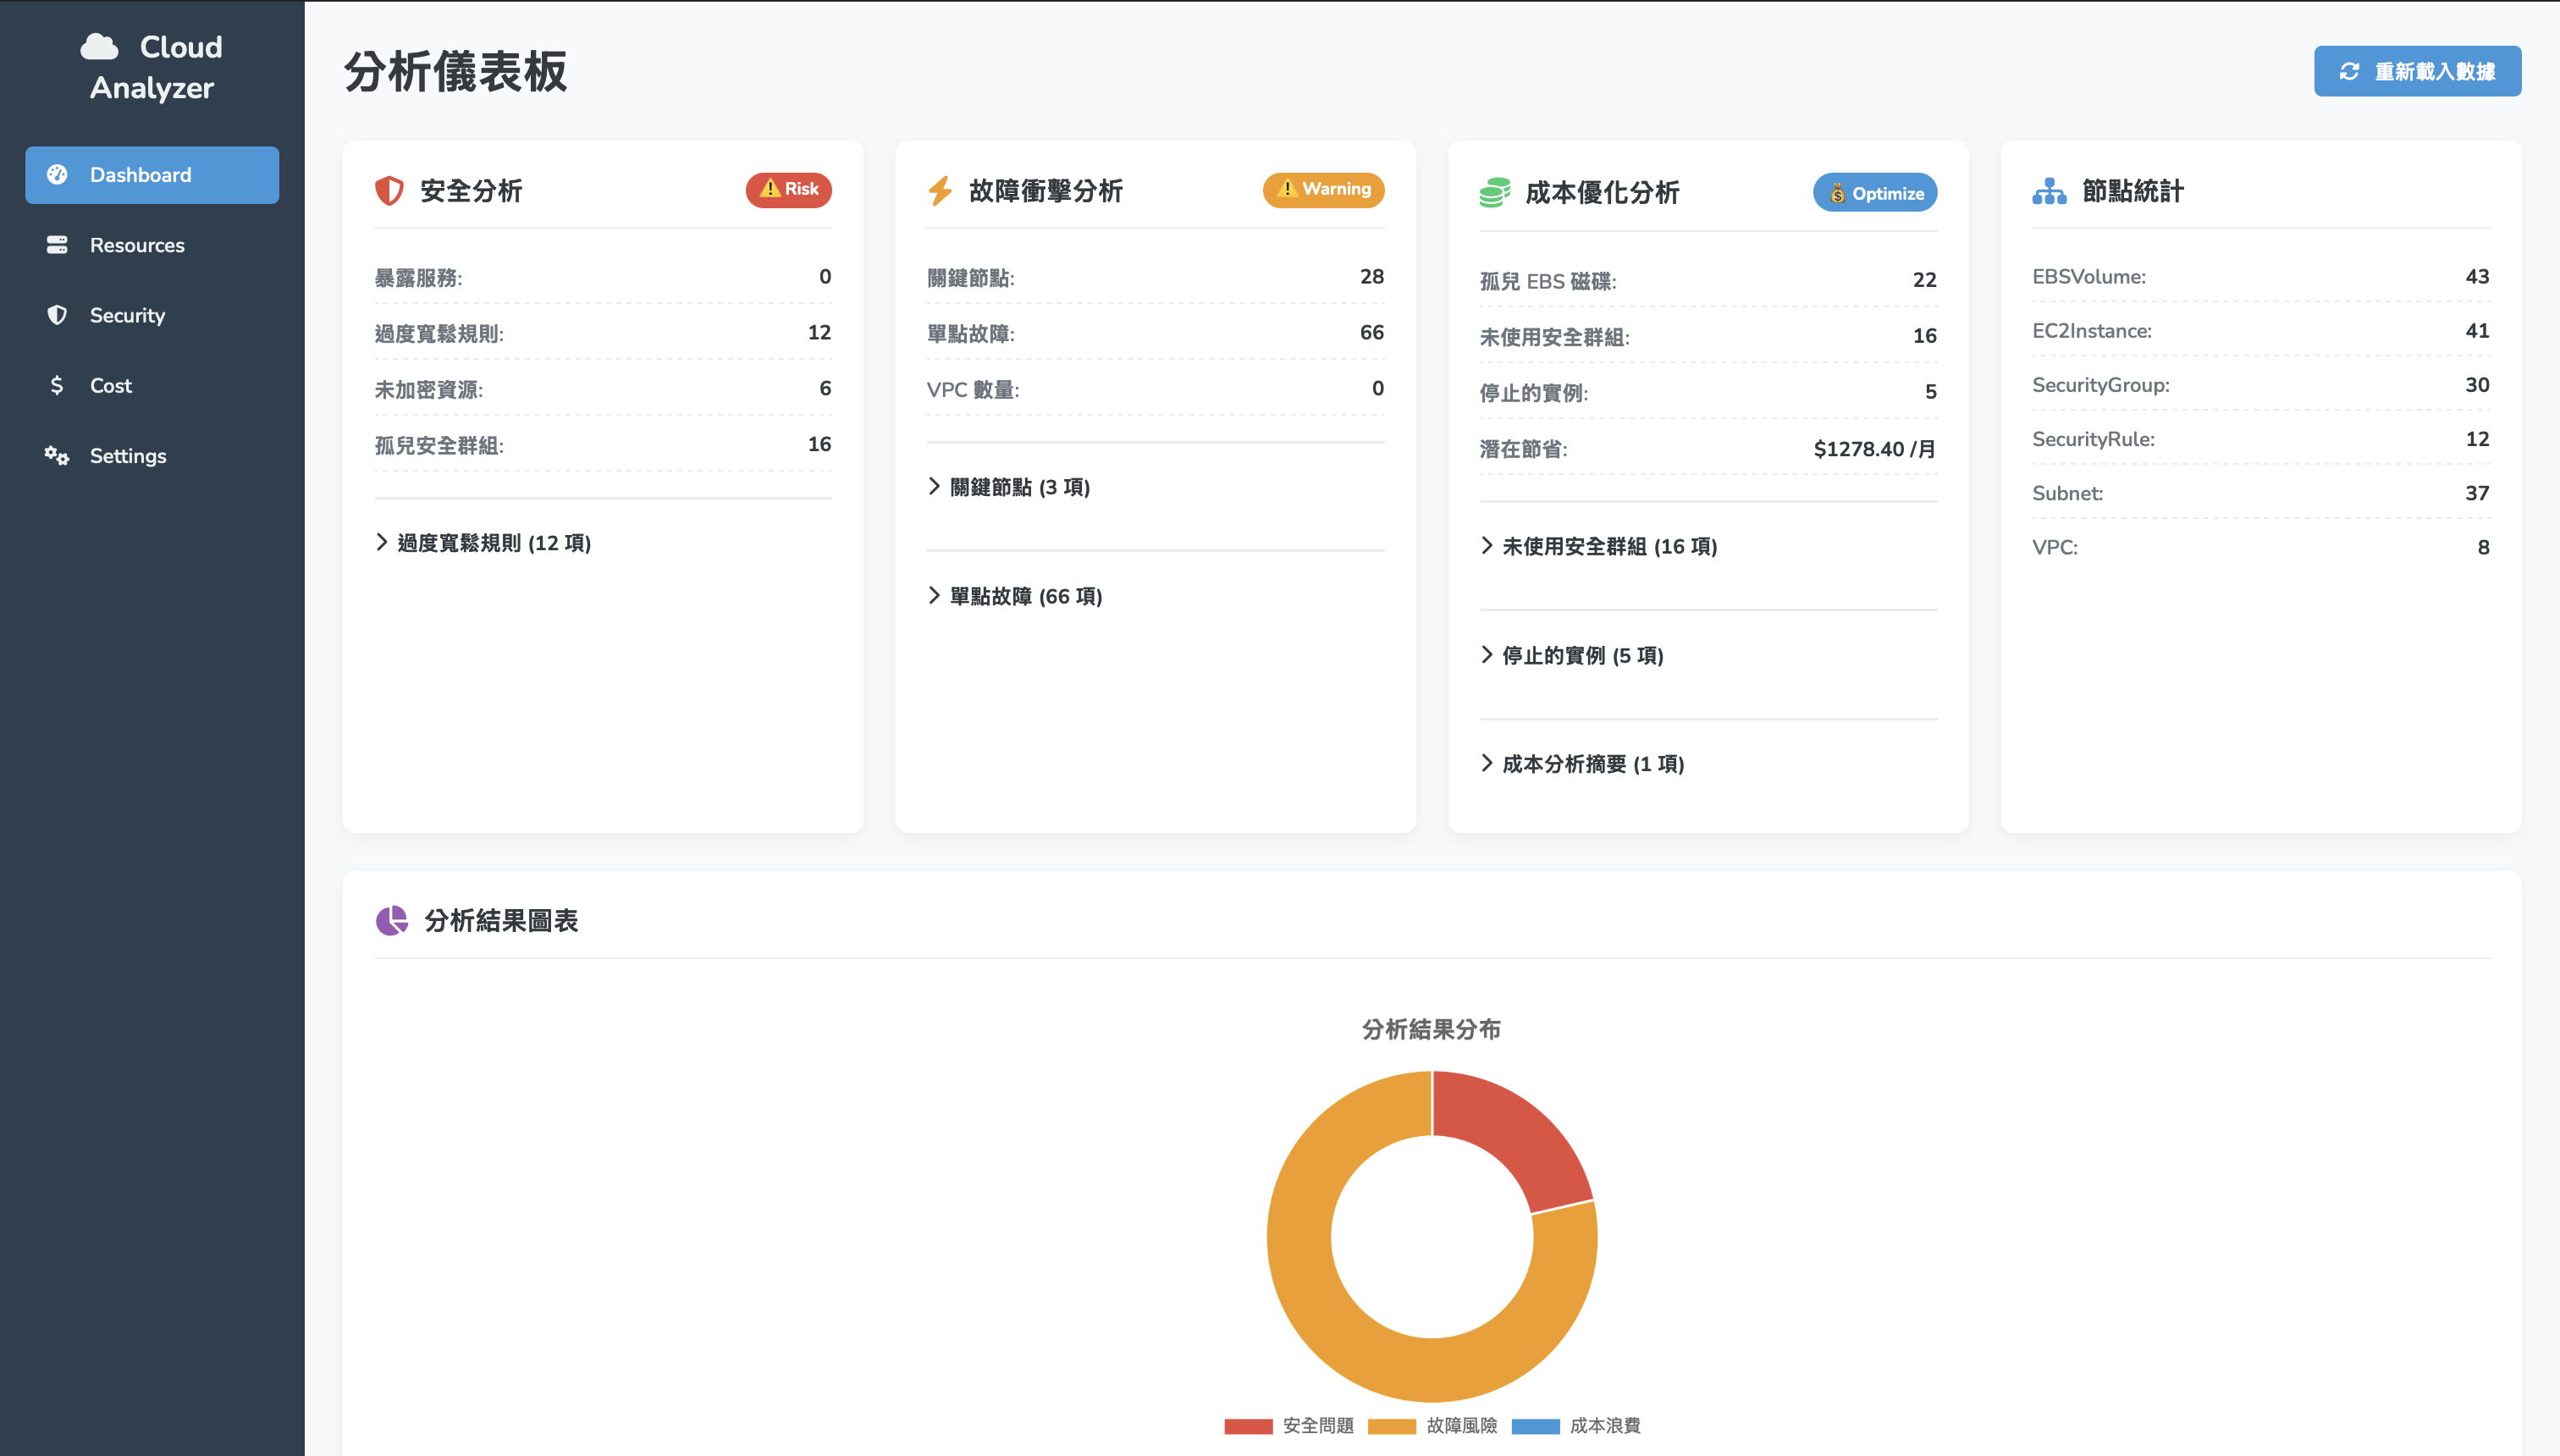
\includegraphics[width=0.8\textwidth]{Mainpage_Screenshot.png}
\caption{系統主頁面 - 顯示整體分析概覽}
\label{fig:mainpage}
\end{figure}

\begin{figure}[H]
\centering
\begin{subfigure}[b]{0.32\textwidth}
\centering
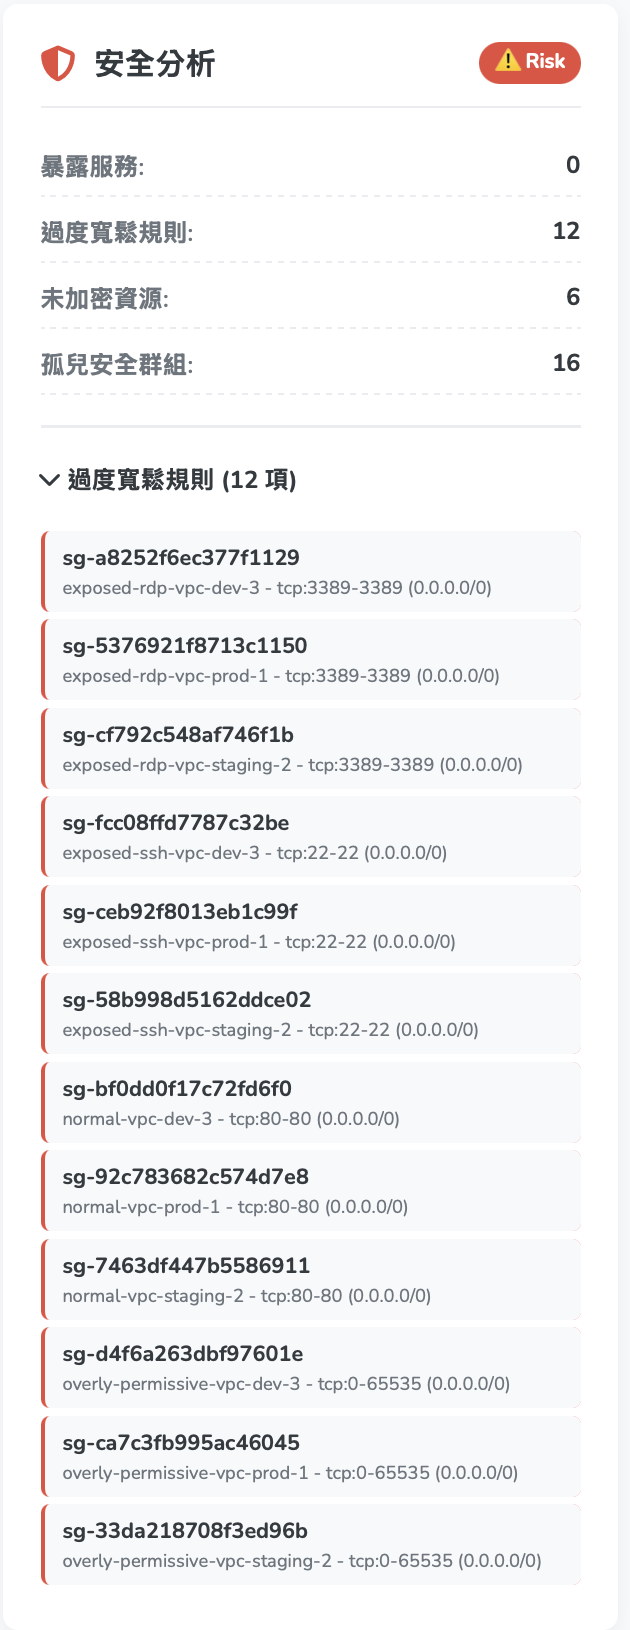
\includegraphics[width=\textwidth]{安全分析.png}
\caption{安全性分析結果}
\label{fig:security}
\end{subfigure}
\hfill
\begin{subfigure}[b]{0.32\textwidth}
\centering
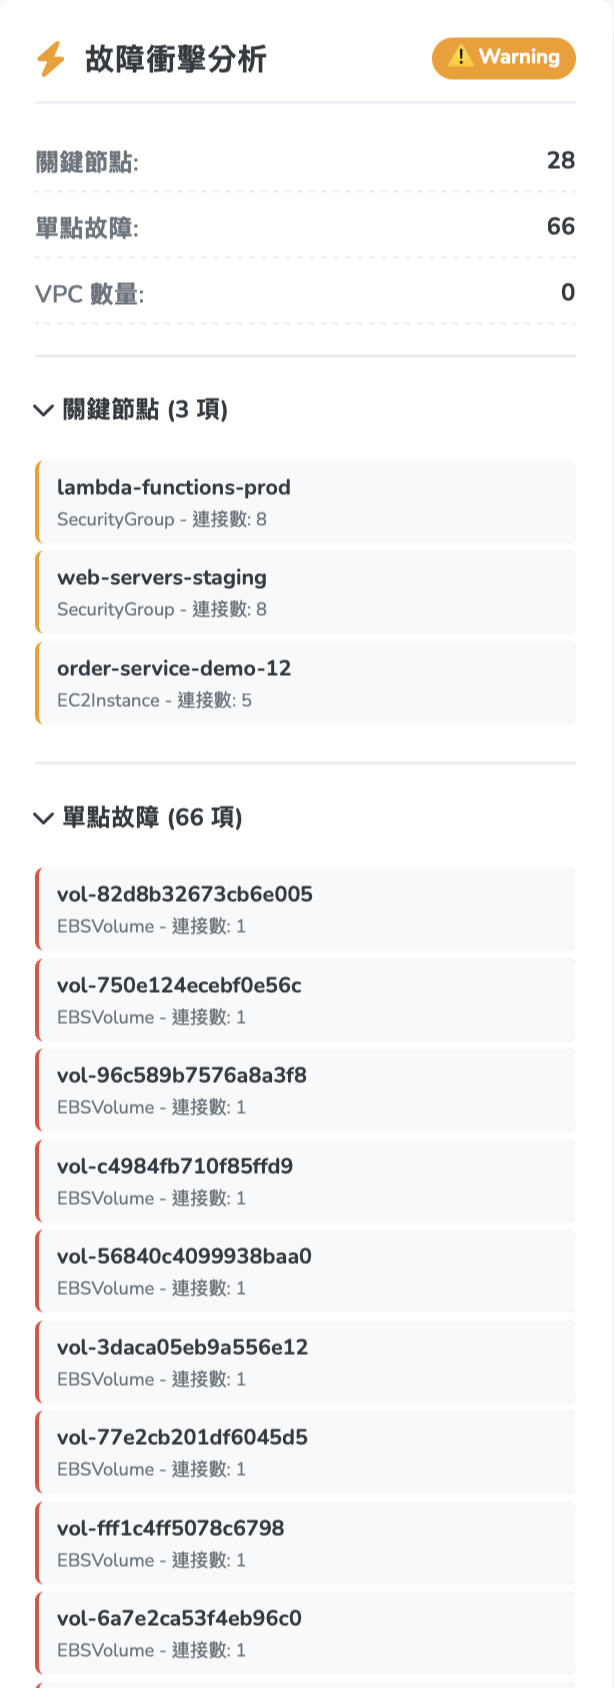
\includegraphics[width=\textwidth]{故障衝擊分析.png}
\caption{故障衝擊分析}
\label{fig:failure}
\end{subfigure}
\hfill
\begin{subfigure}[b]{0.32\textwidth}
\centering
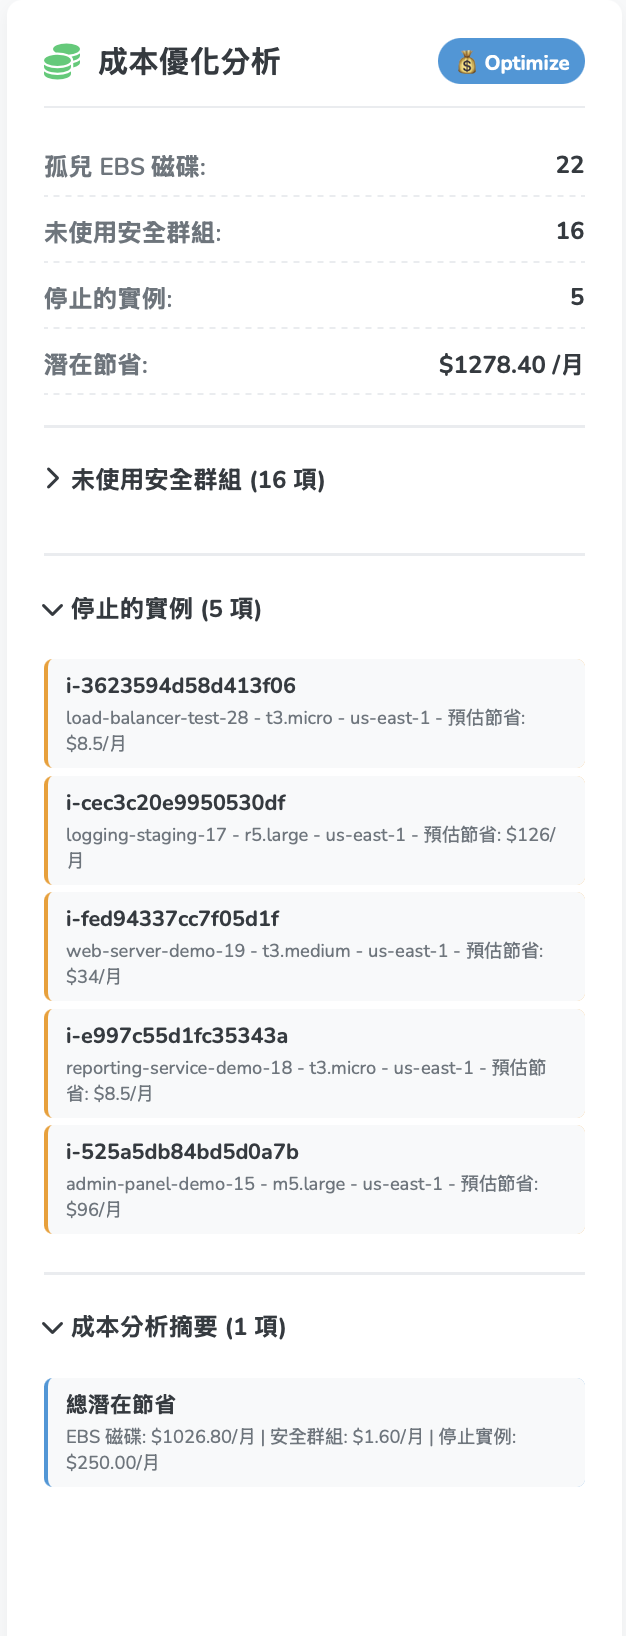
\includegraphics[width=\textwidth]{成本優化分析.png}
\caption{成本優化分析}
\label{fig:cost}
\end{subfigure}
\caption{三大核心分析功能截圖 - 安全性分析、故障衝擊分析、成本優化分析}
\label{fig:analysis_screenshots}
\end{figure}

\begin{figure}[H]
\centering
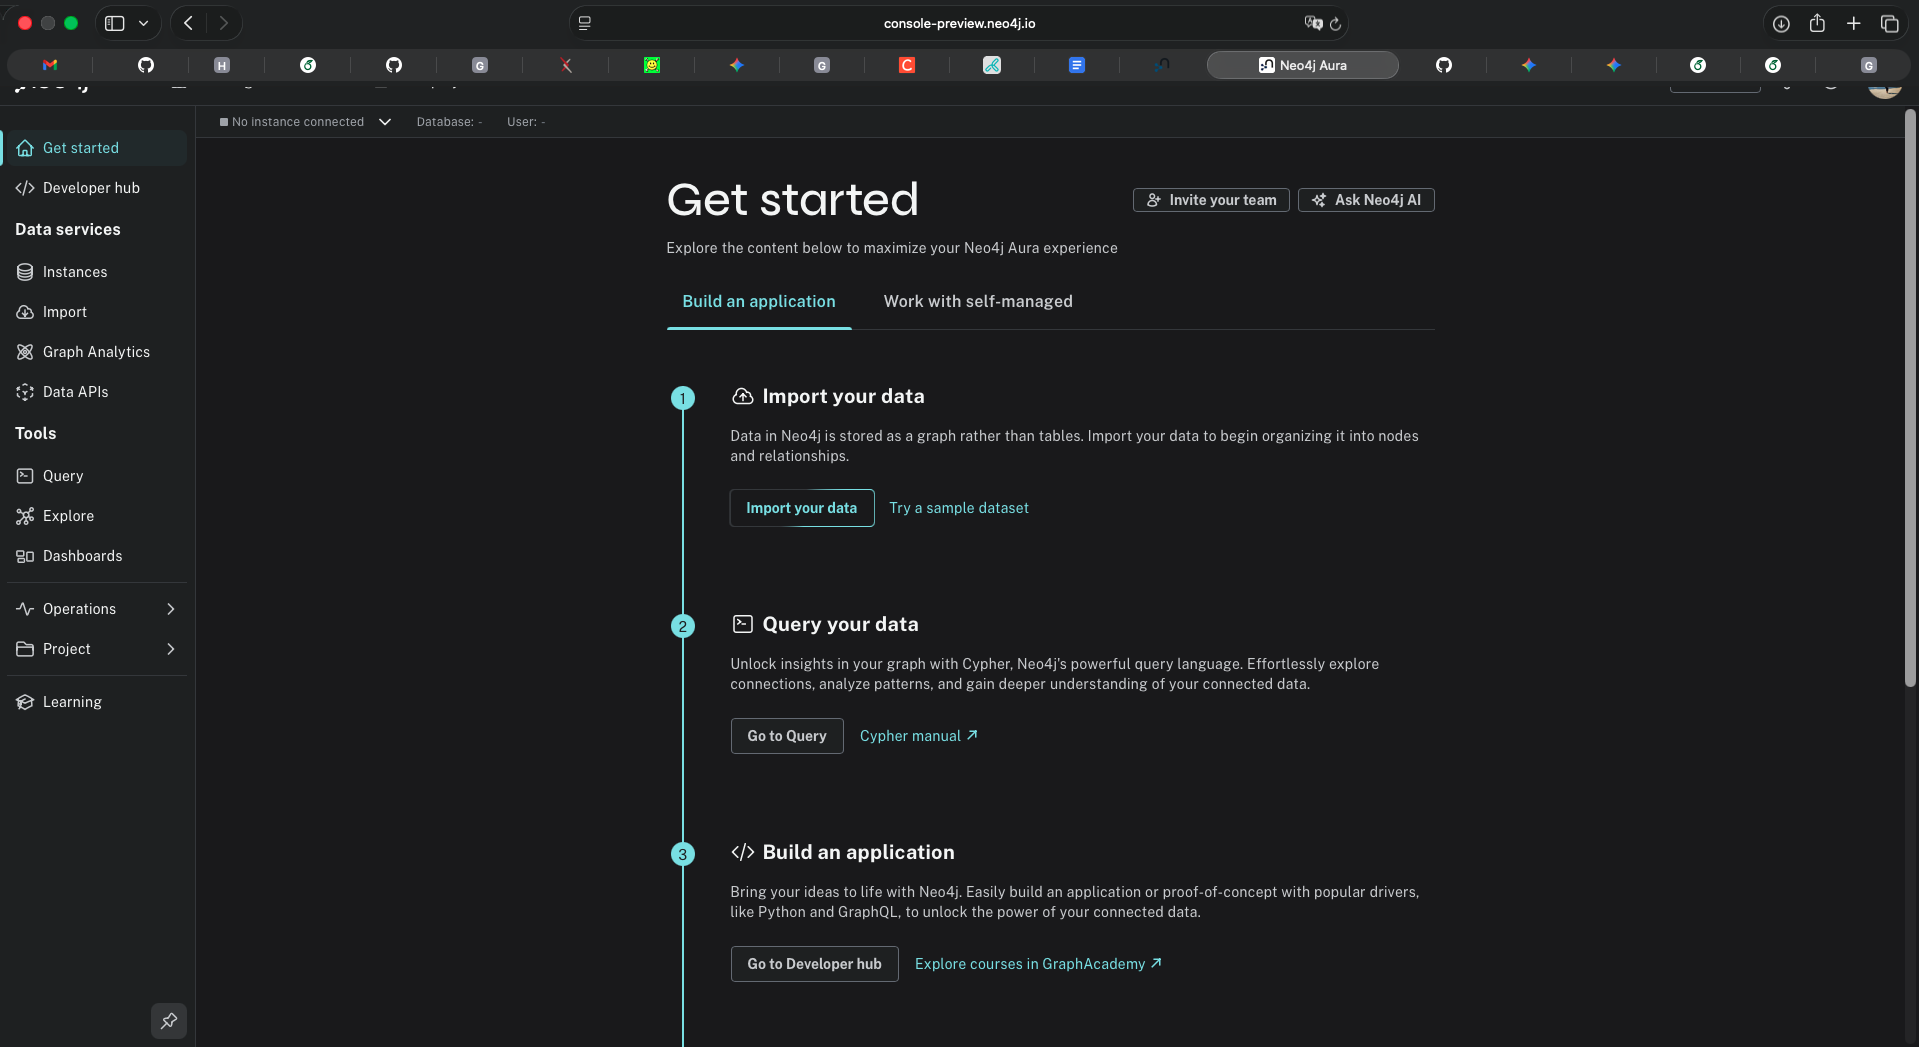
\includegraphics[width=0.6\textwidth]{neo4j_aura.png}
\caption{Neo4j Aura 雲端資料庫 - 圖形資料儲存和查詢}
\label{fig:neo4j}
\end{figure}

\subsection{Neo4j 查詢結果展示}

本節展示在 Neo4j Aura 中執行的各種 Cypher 查詢結果,驗證系統的分析功能。

\subsubsection{節點類型查詢結果}

\begin{figure}[H]
\centering
\begin{subfigure}[b]{0.48\textwidth}
\centering
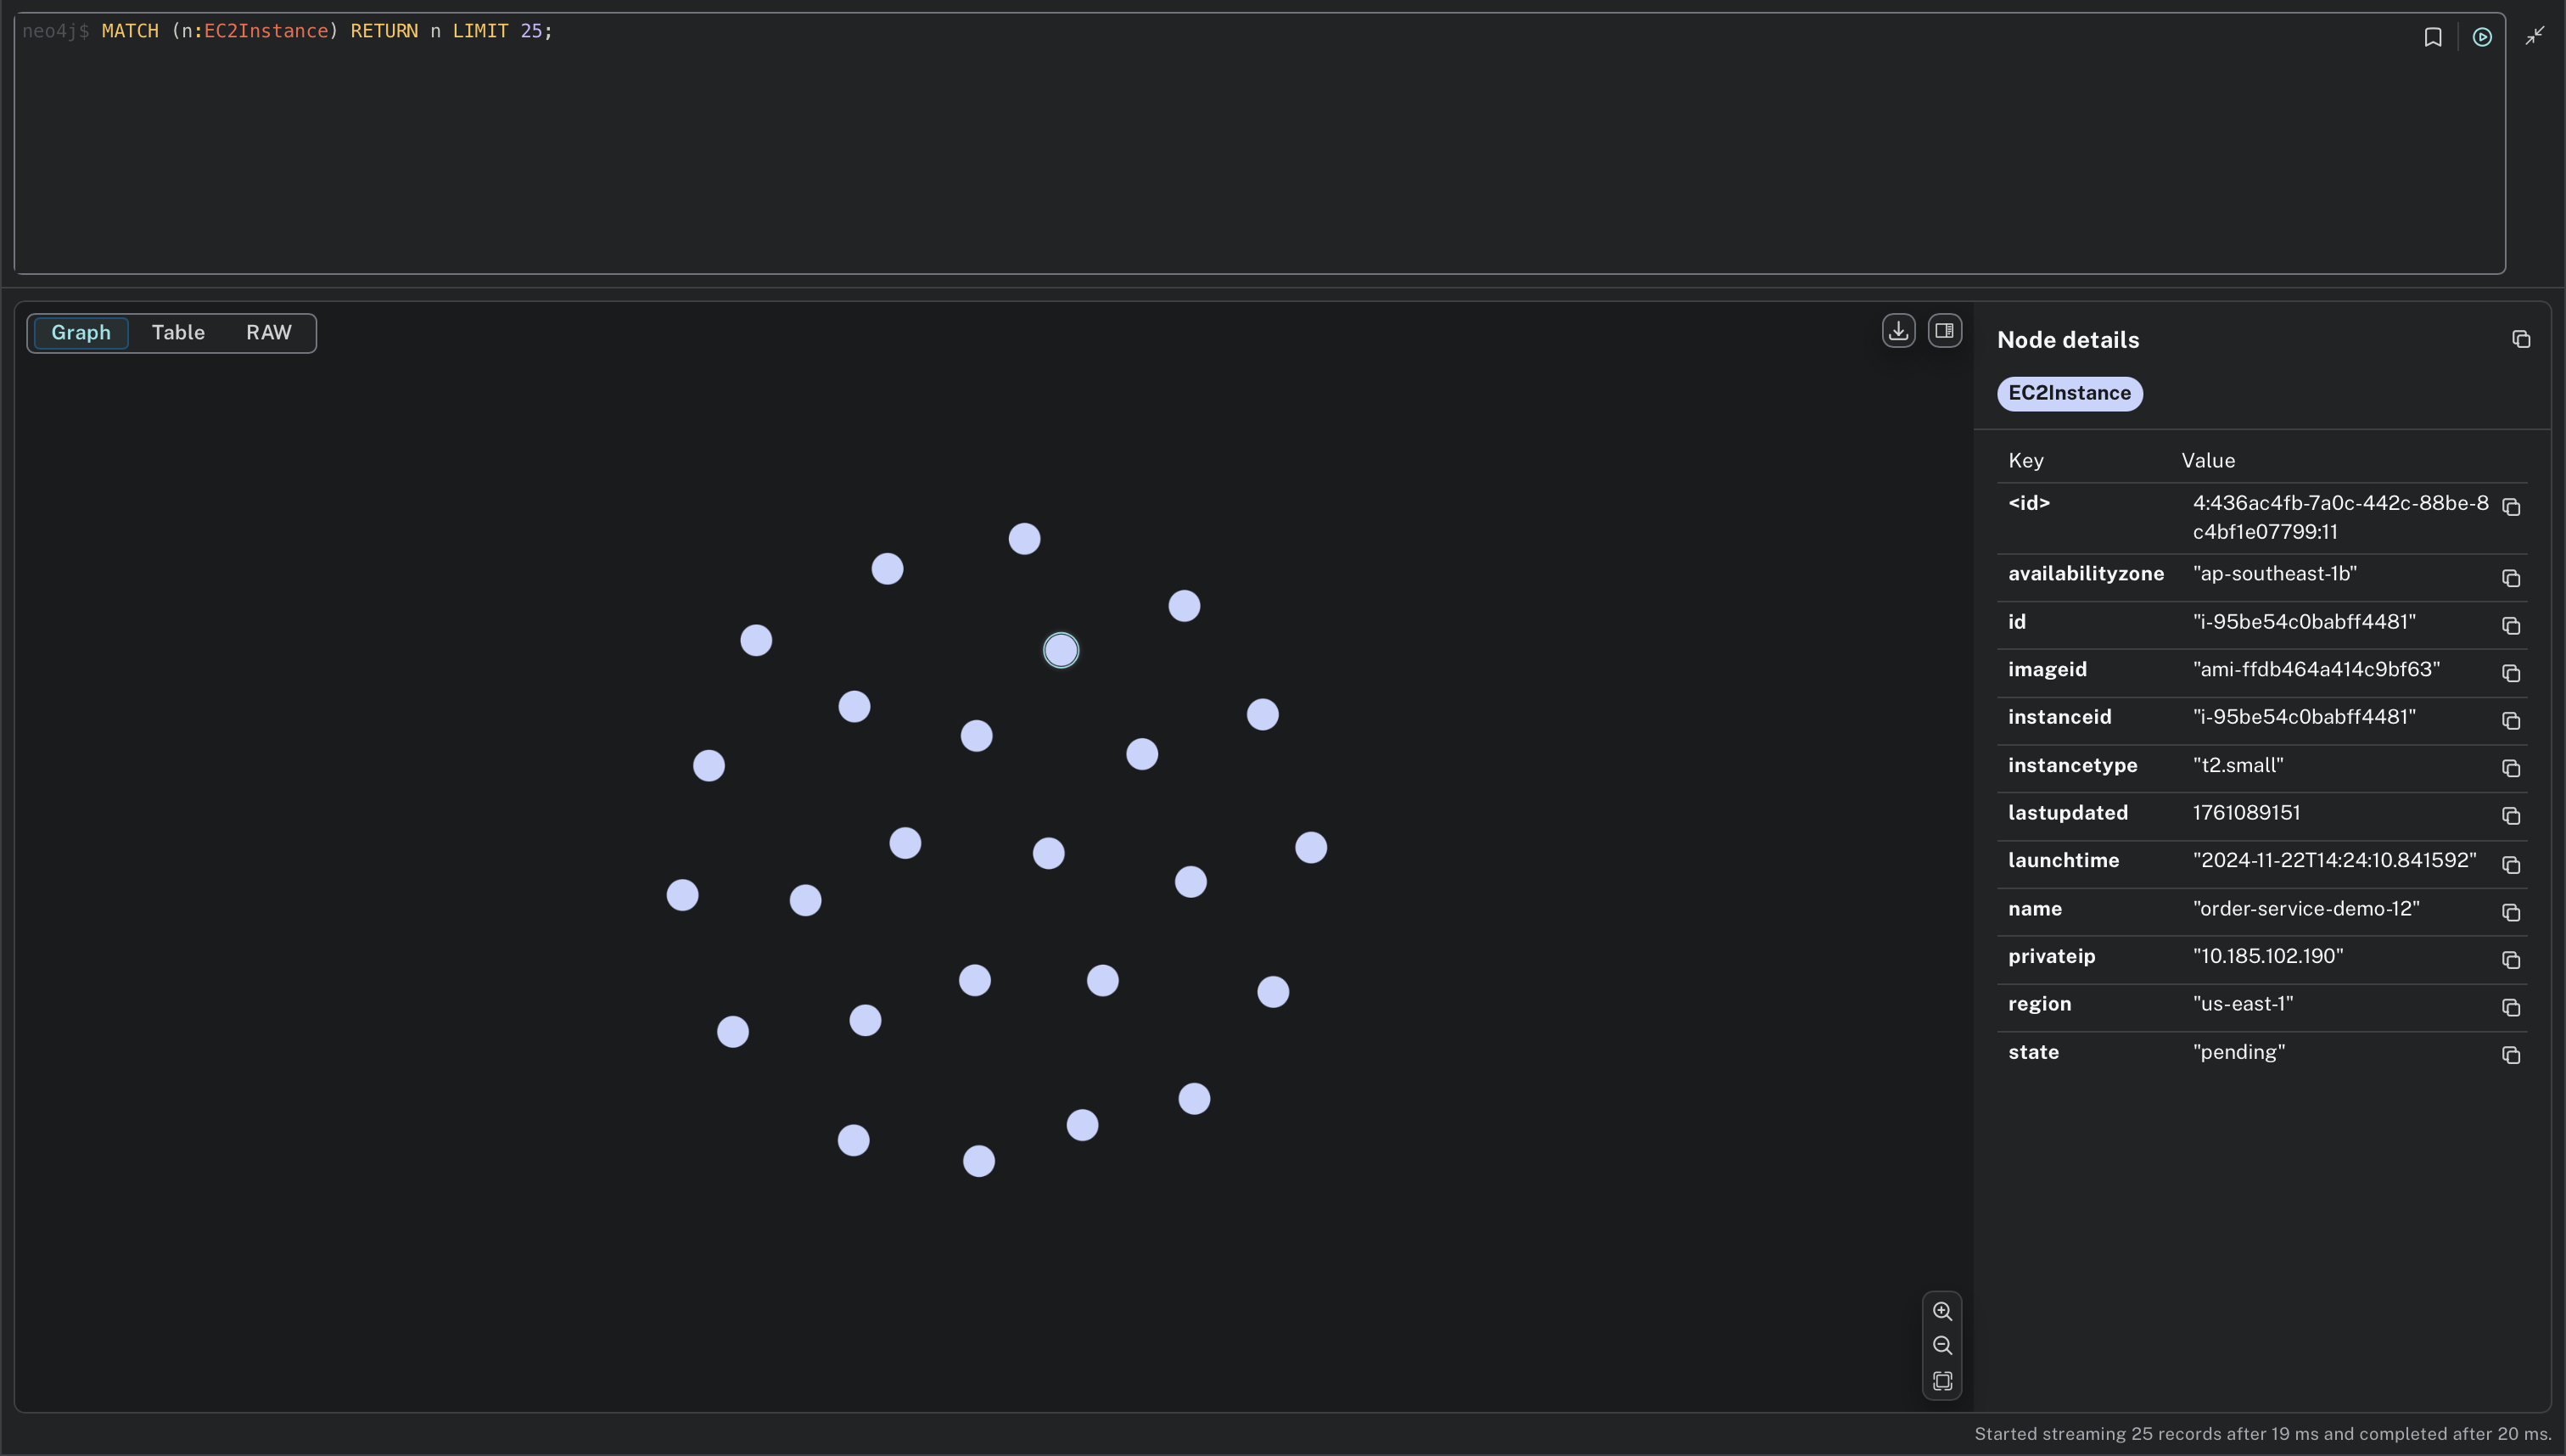
\includegraphics[width=\textwidth]{EC2Instances.png}
\caption{EC2 實例節點}
\label{fig:ec2_nodes}
\end{subfigure}
\hfill
\begin{subfigure}[b]{0.48\textwidth}
\centering
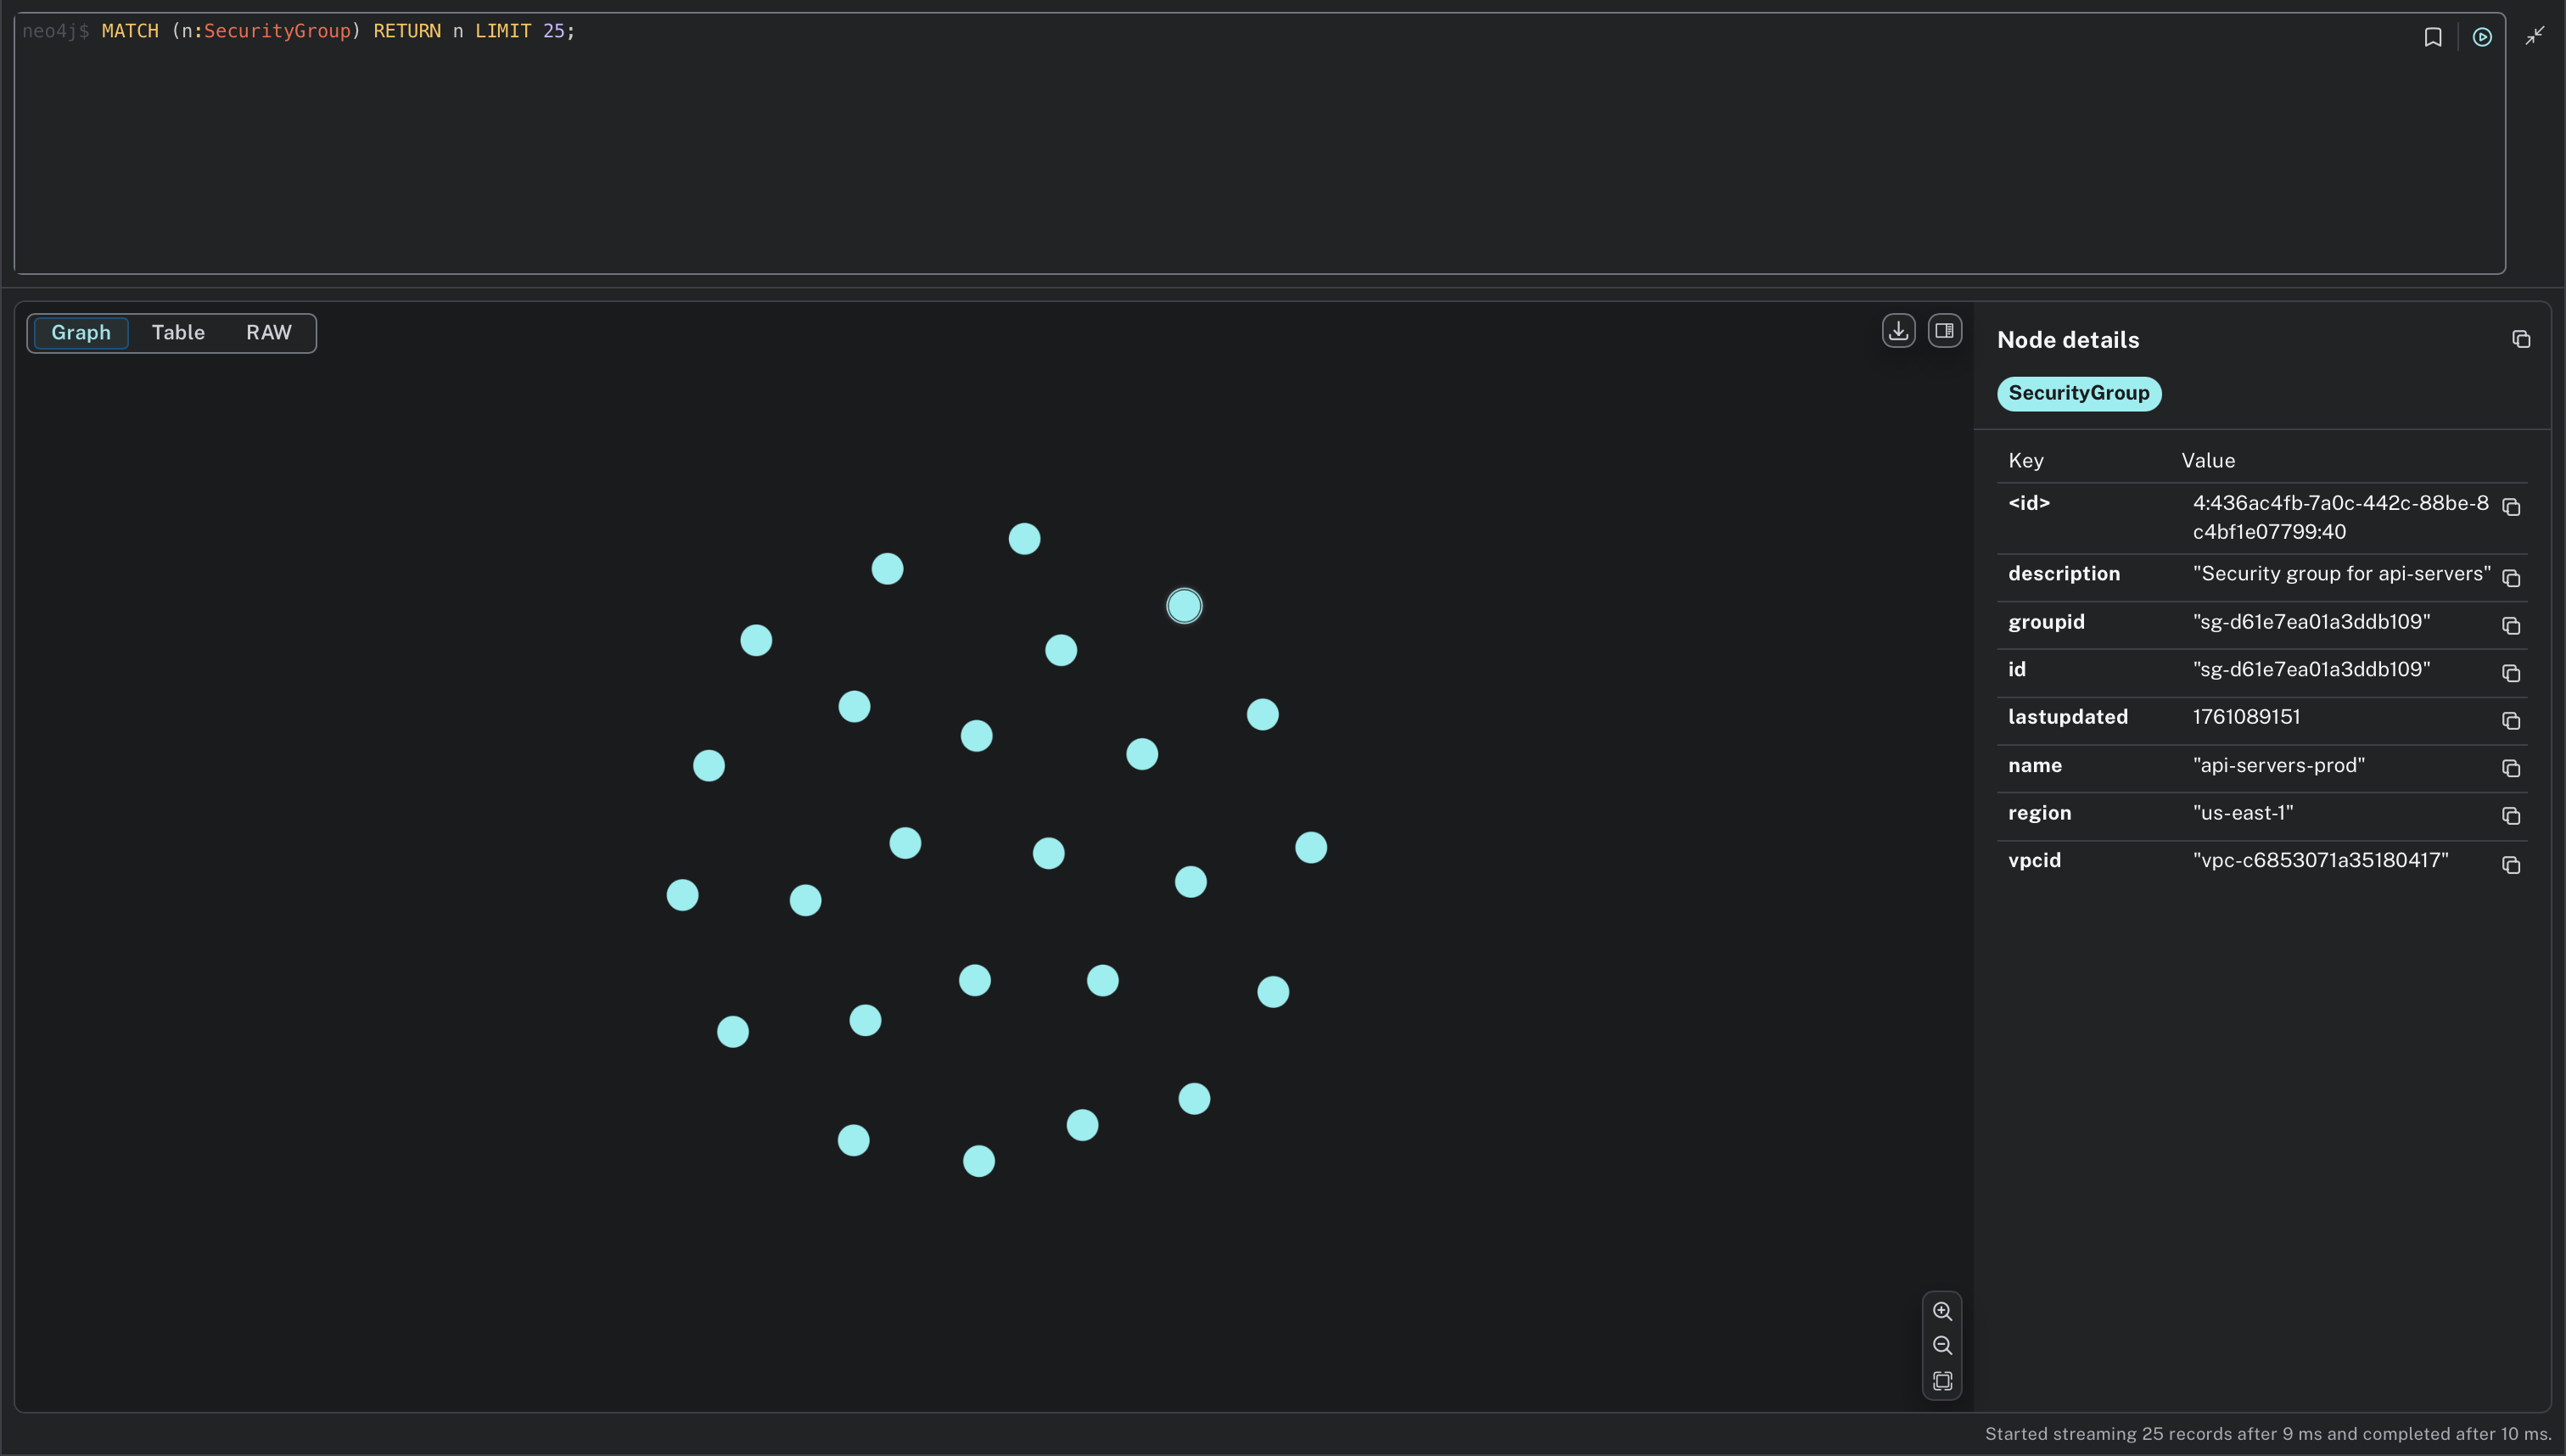
\includegraphics[width=\textwidth]{SecurityGroup.png}
\caption{安全群組節點}
\label{fig:sg_nodes}
\end{subfigure}
\caption{核心節點類型查詢結果}
\label{fig:node_types}
\end{figure}

\begin{figure}[H]
\centering
\begin{subfigure}[b]{0.48\textwidth}
\centering
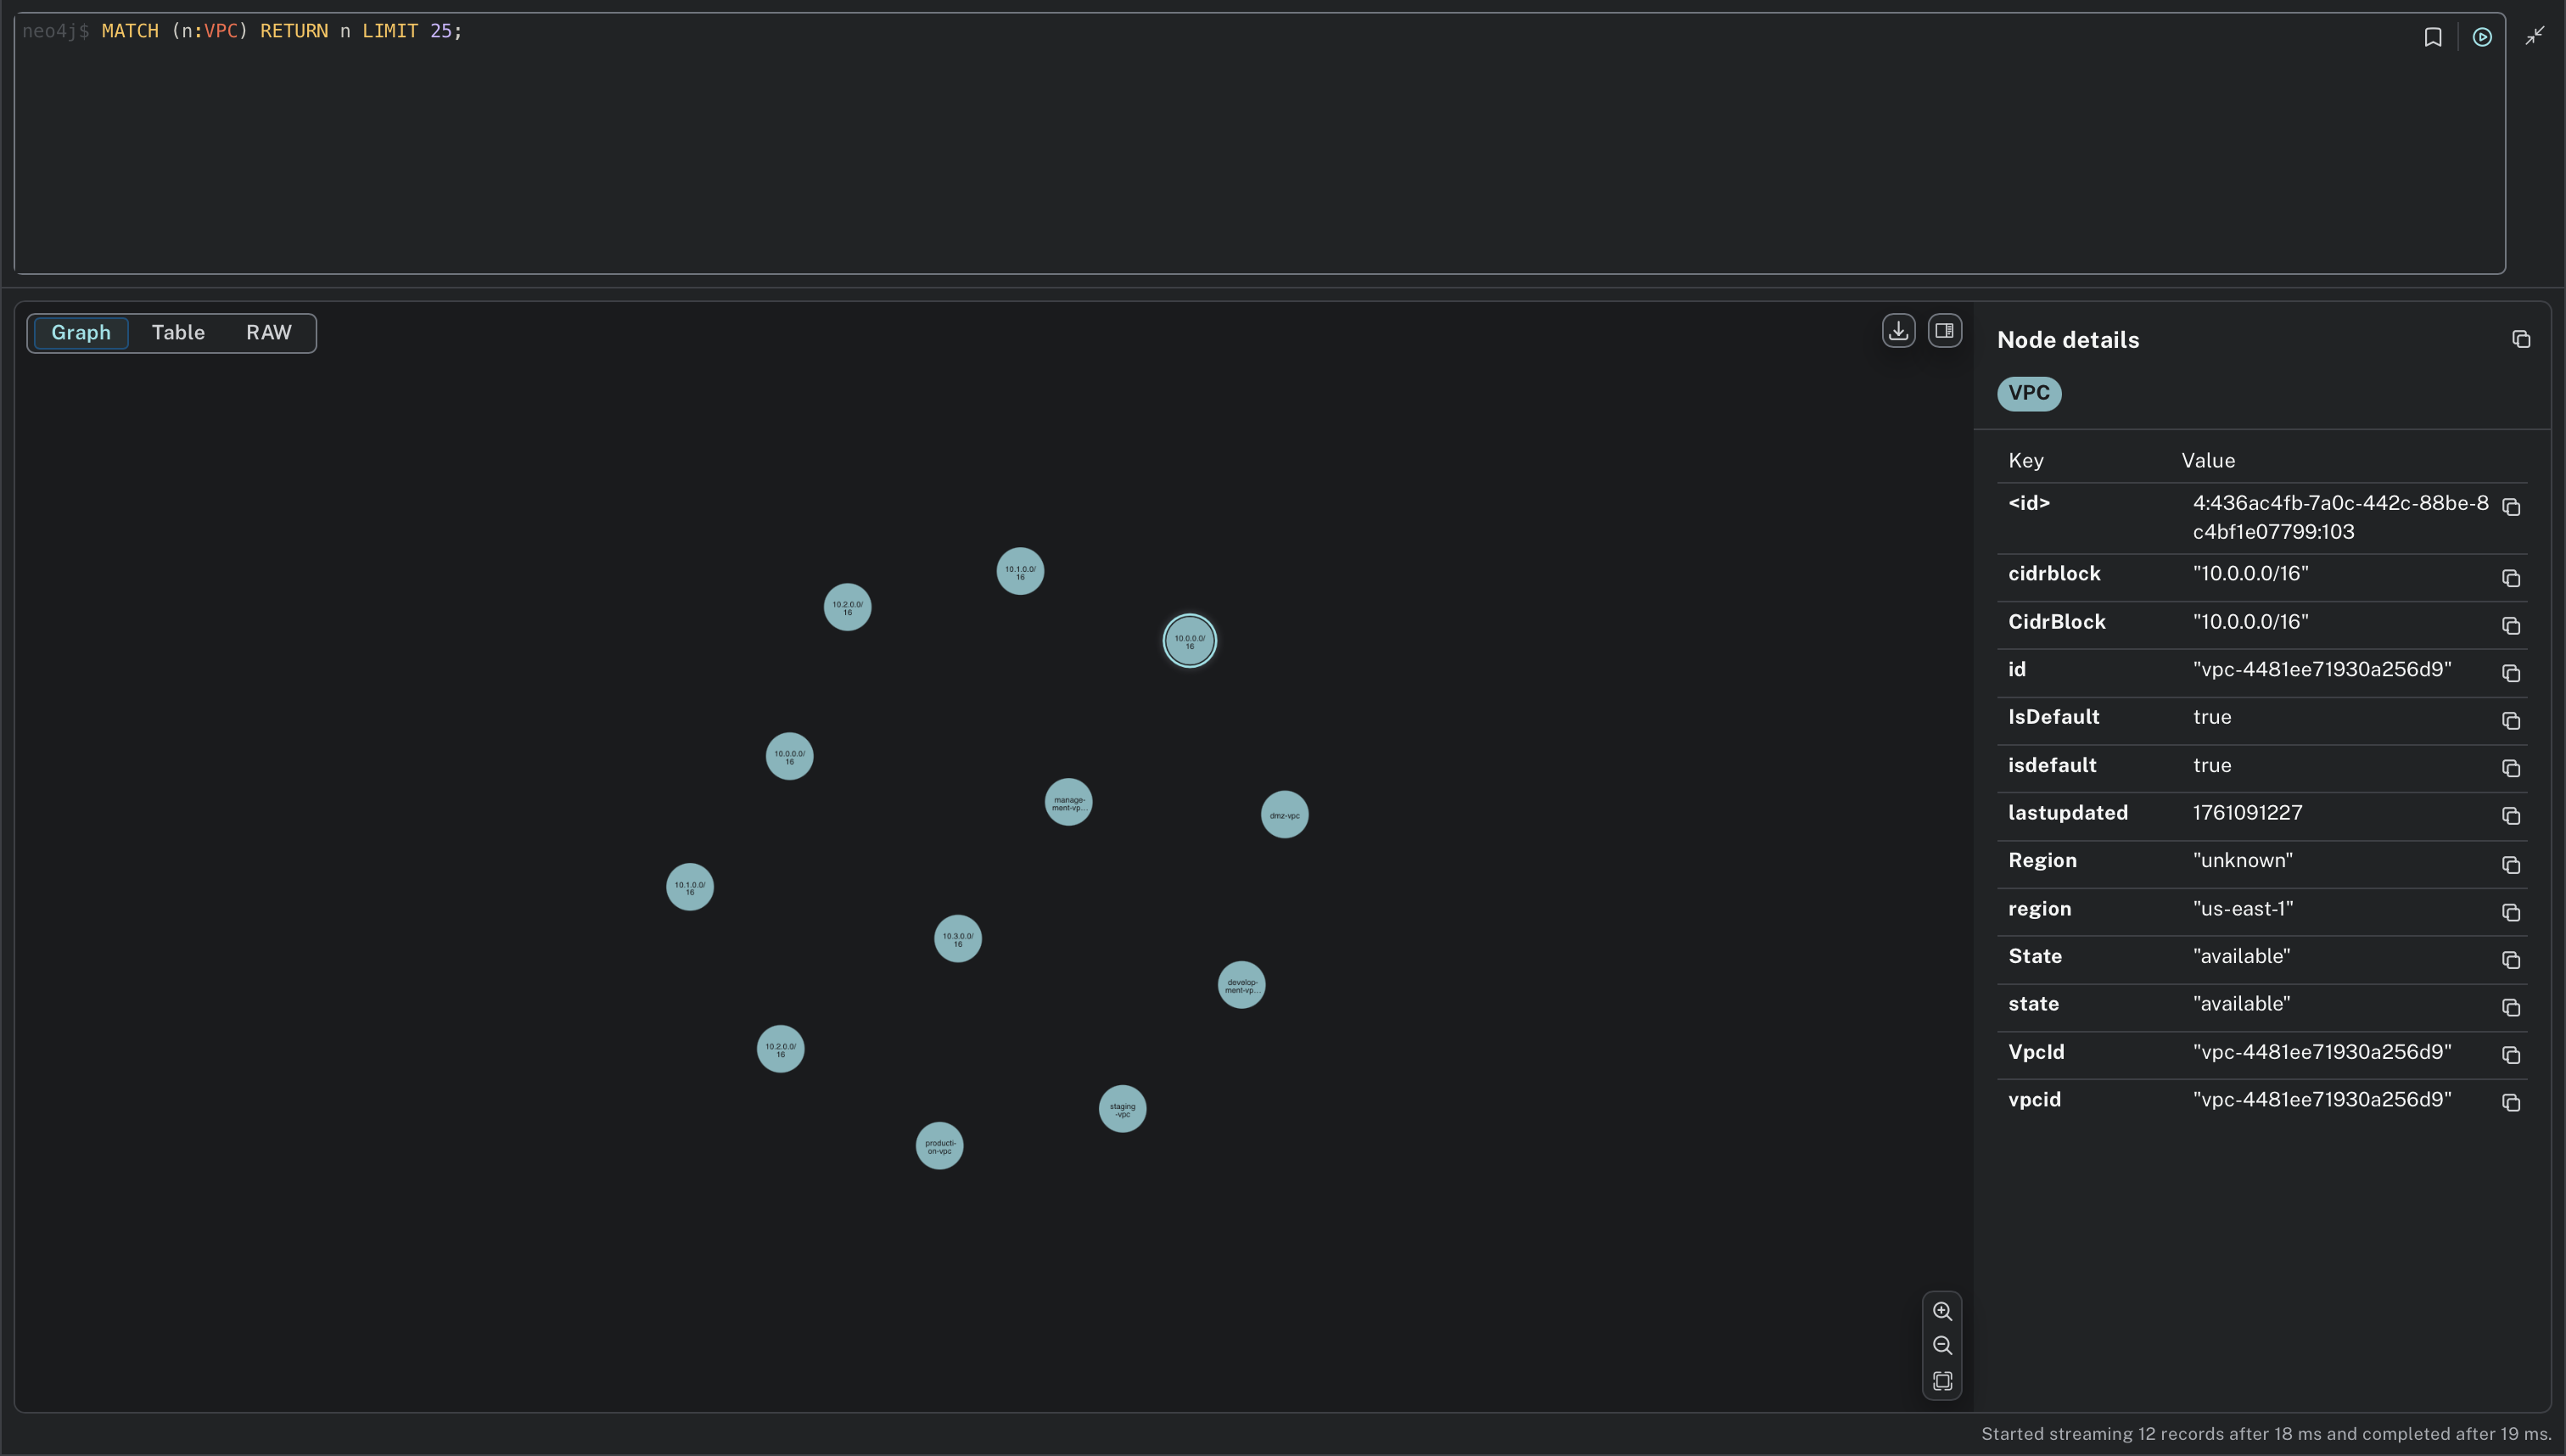
\includegraphics[width=\textwidth]{VPC.png}
\caption{VPC 節點}
\label{fig:vpc_nodes}
\end{subfigure}
\hfill
\begin{subfigure}[b]{0.48\textwidth}
\centering
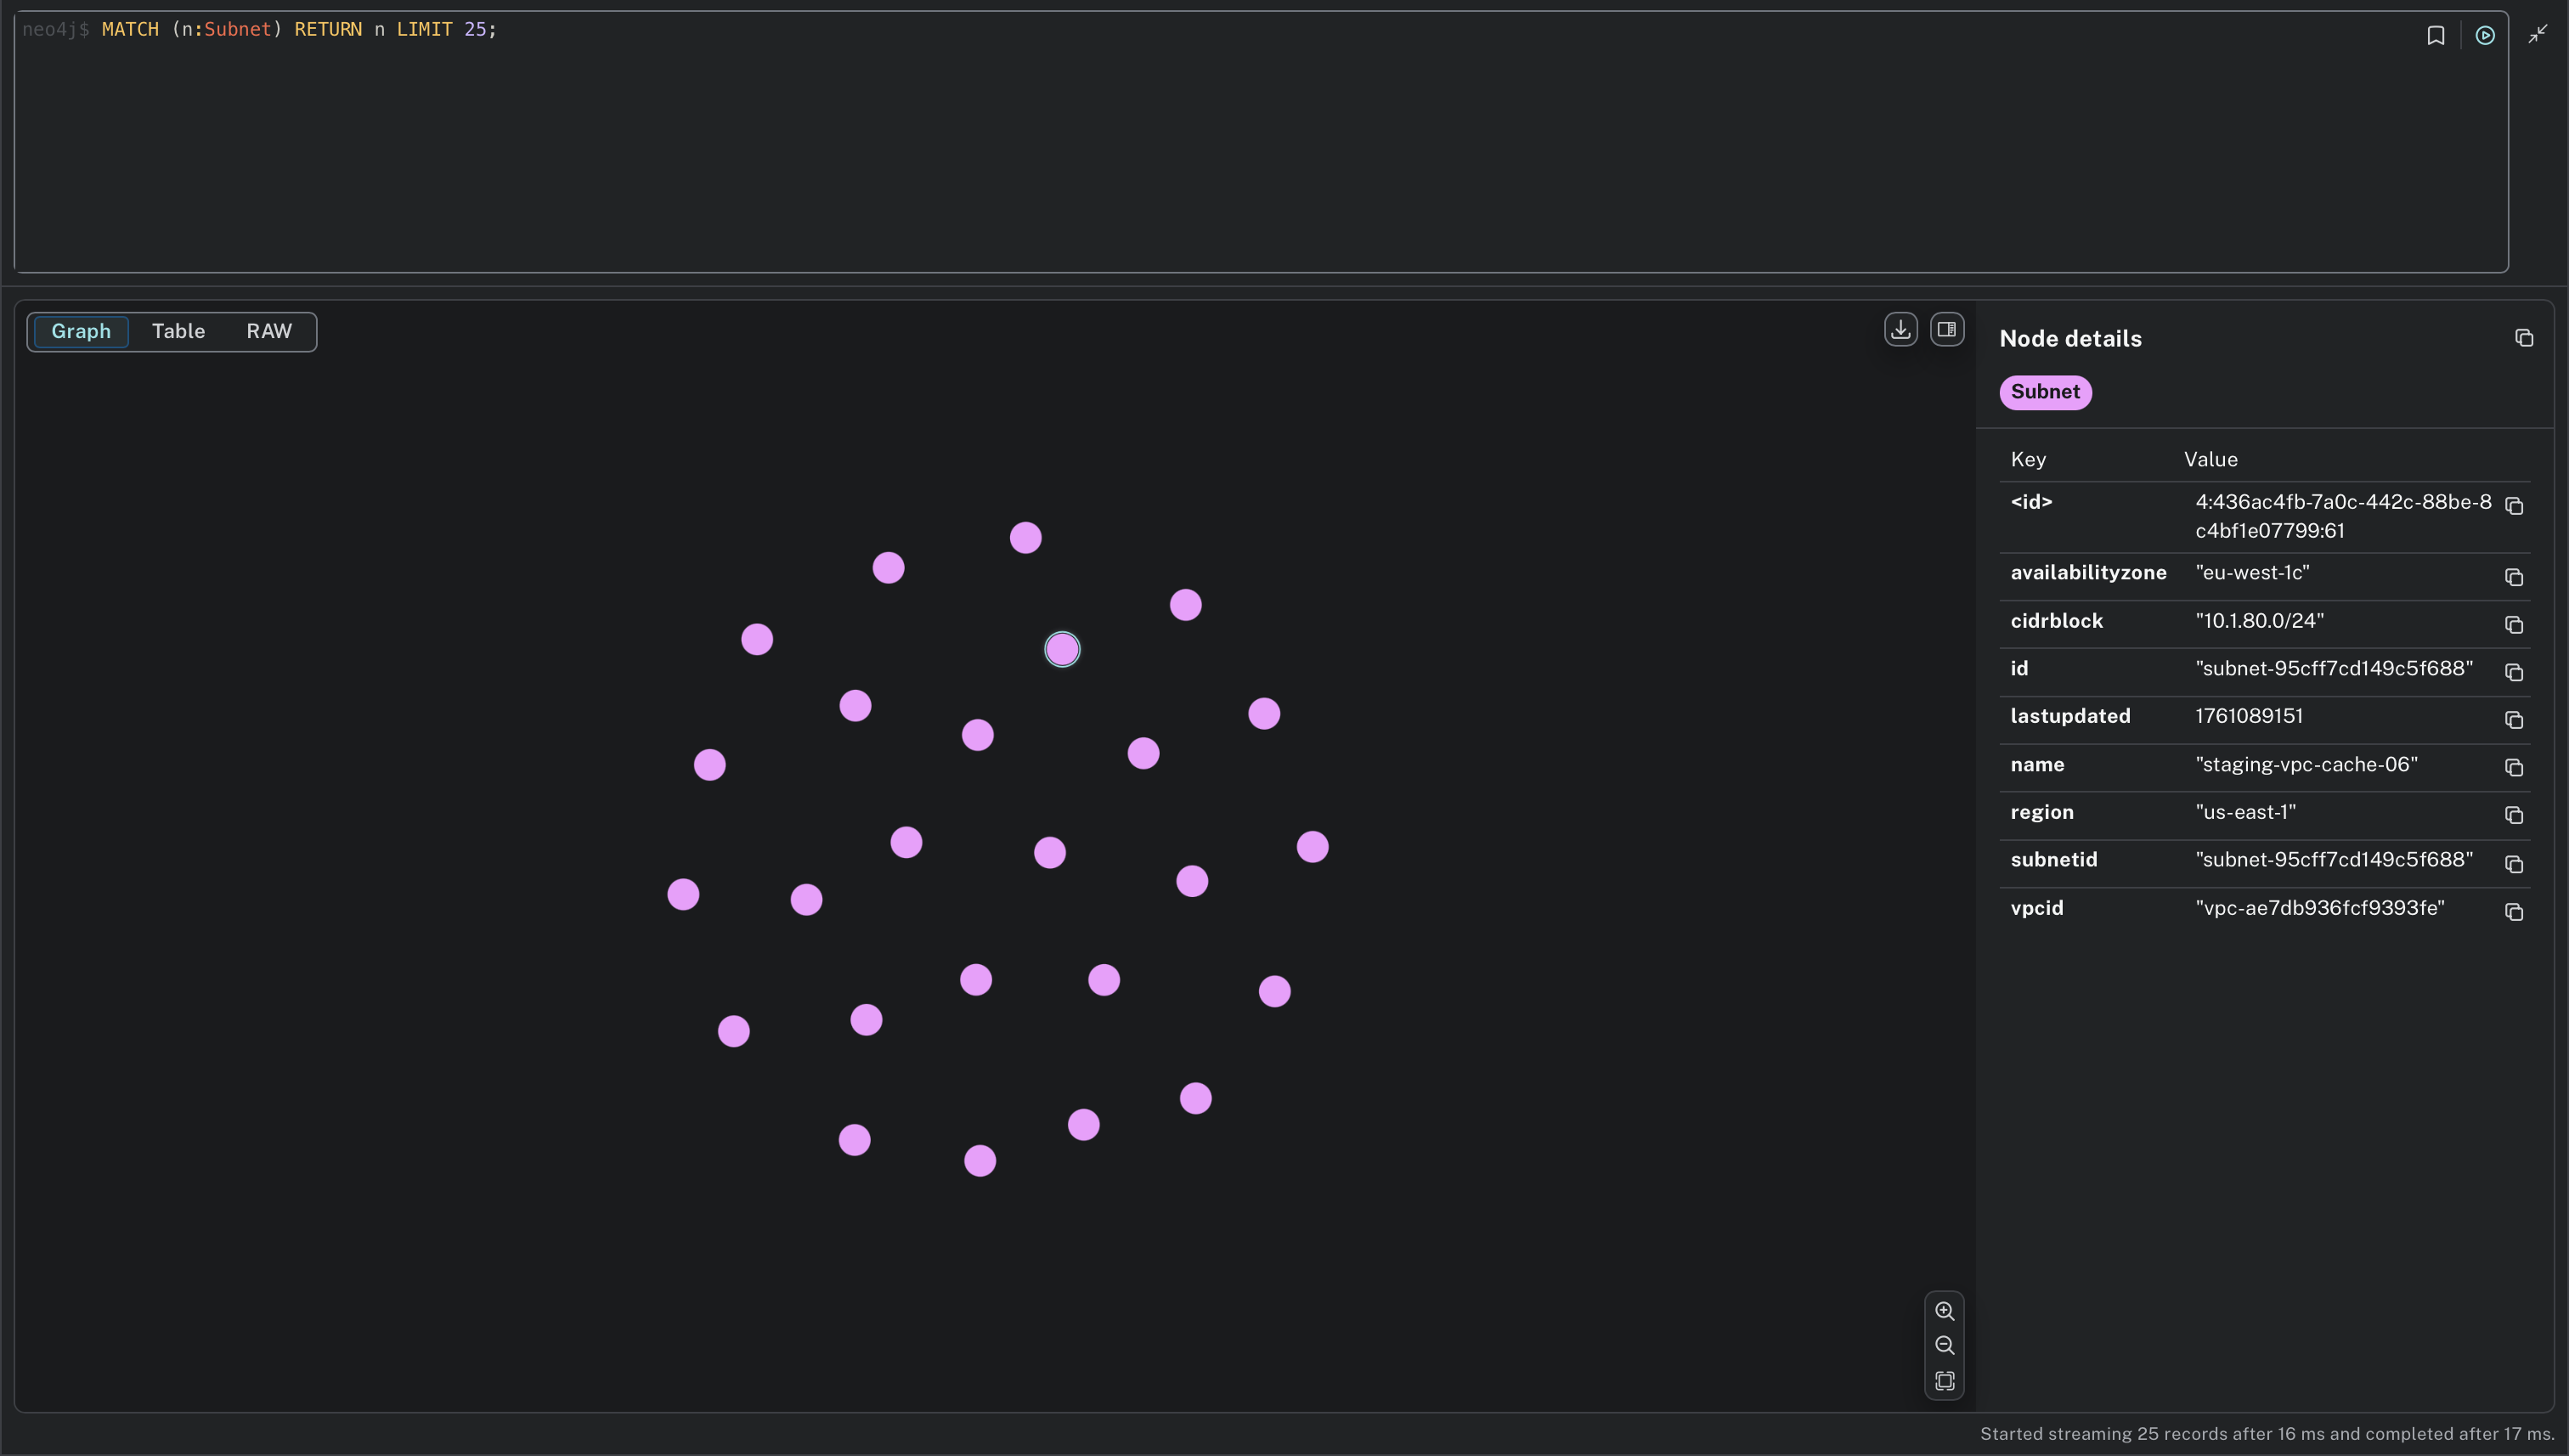
\includegraphics[width=\textwidth]{Subnet.png}
\caption{子網路節點}
\label{fig:subnet_nodes}
\end{subfigure}
\caption{網路基礎設施節點}
\label{fig:network_nodes}
\end{figure}

\begin{figure}[H]
\centering
\begin{subfigure}[b]{0.48\textwidth}
\centering
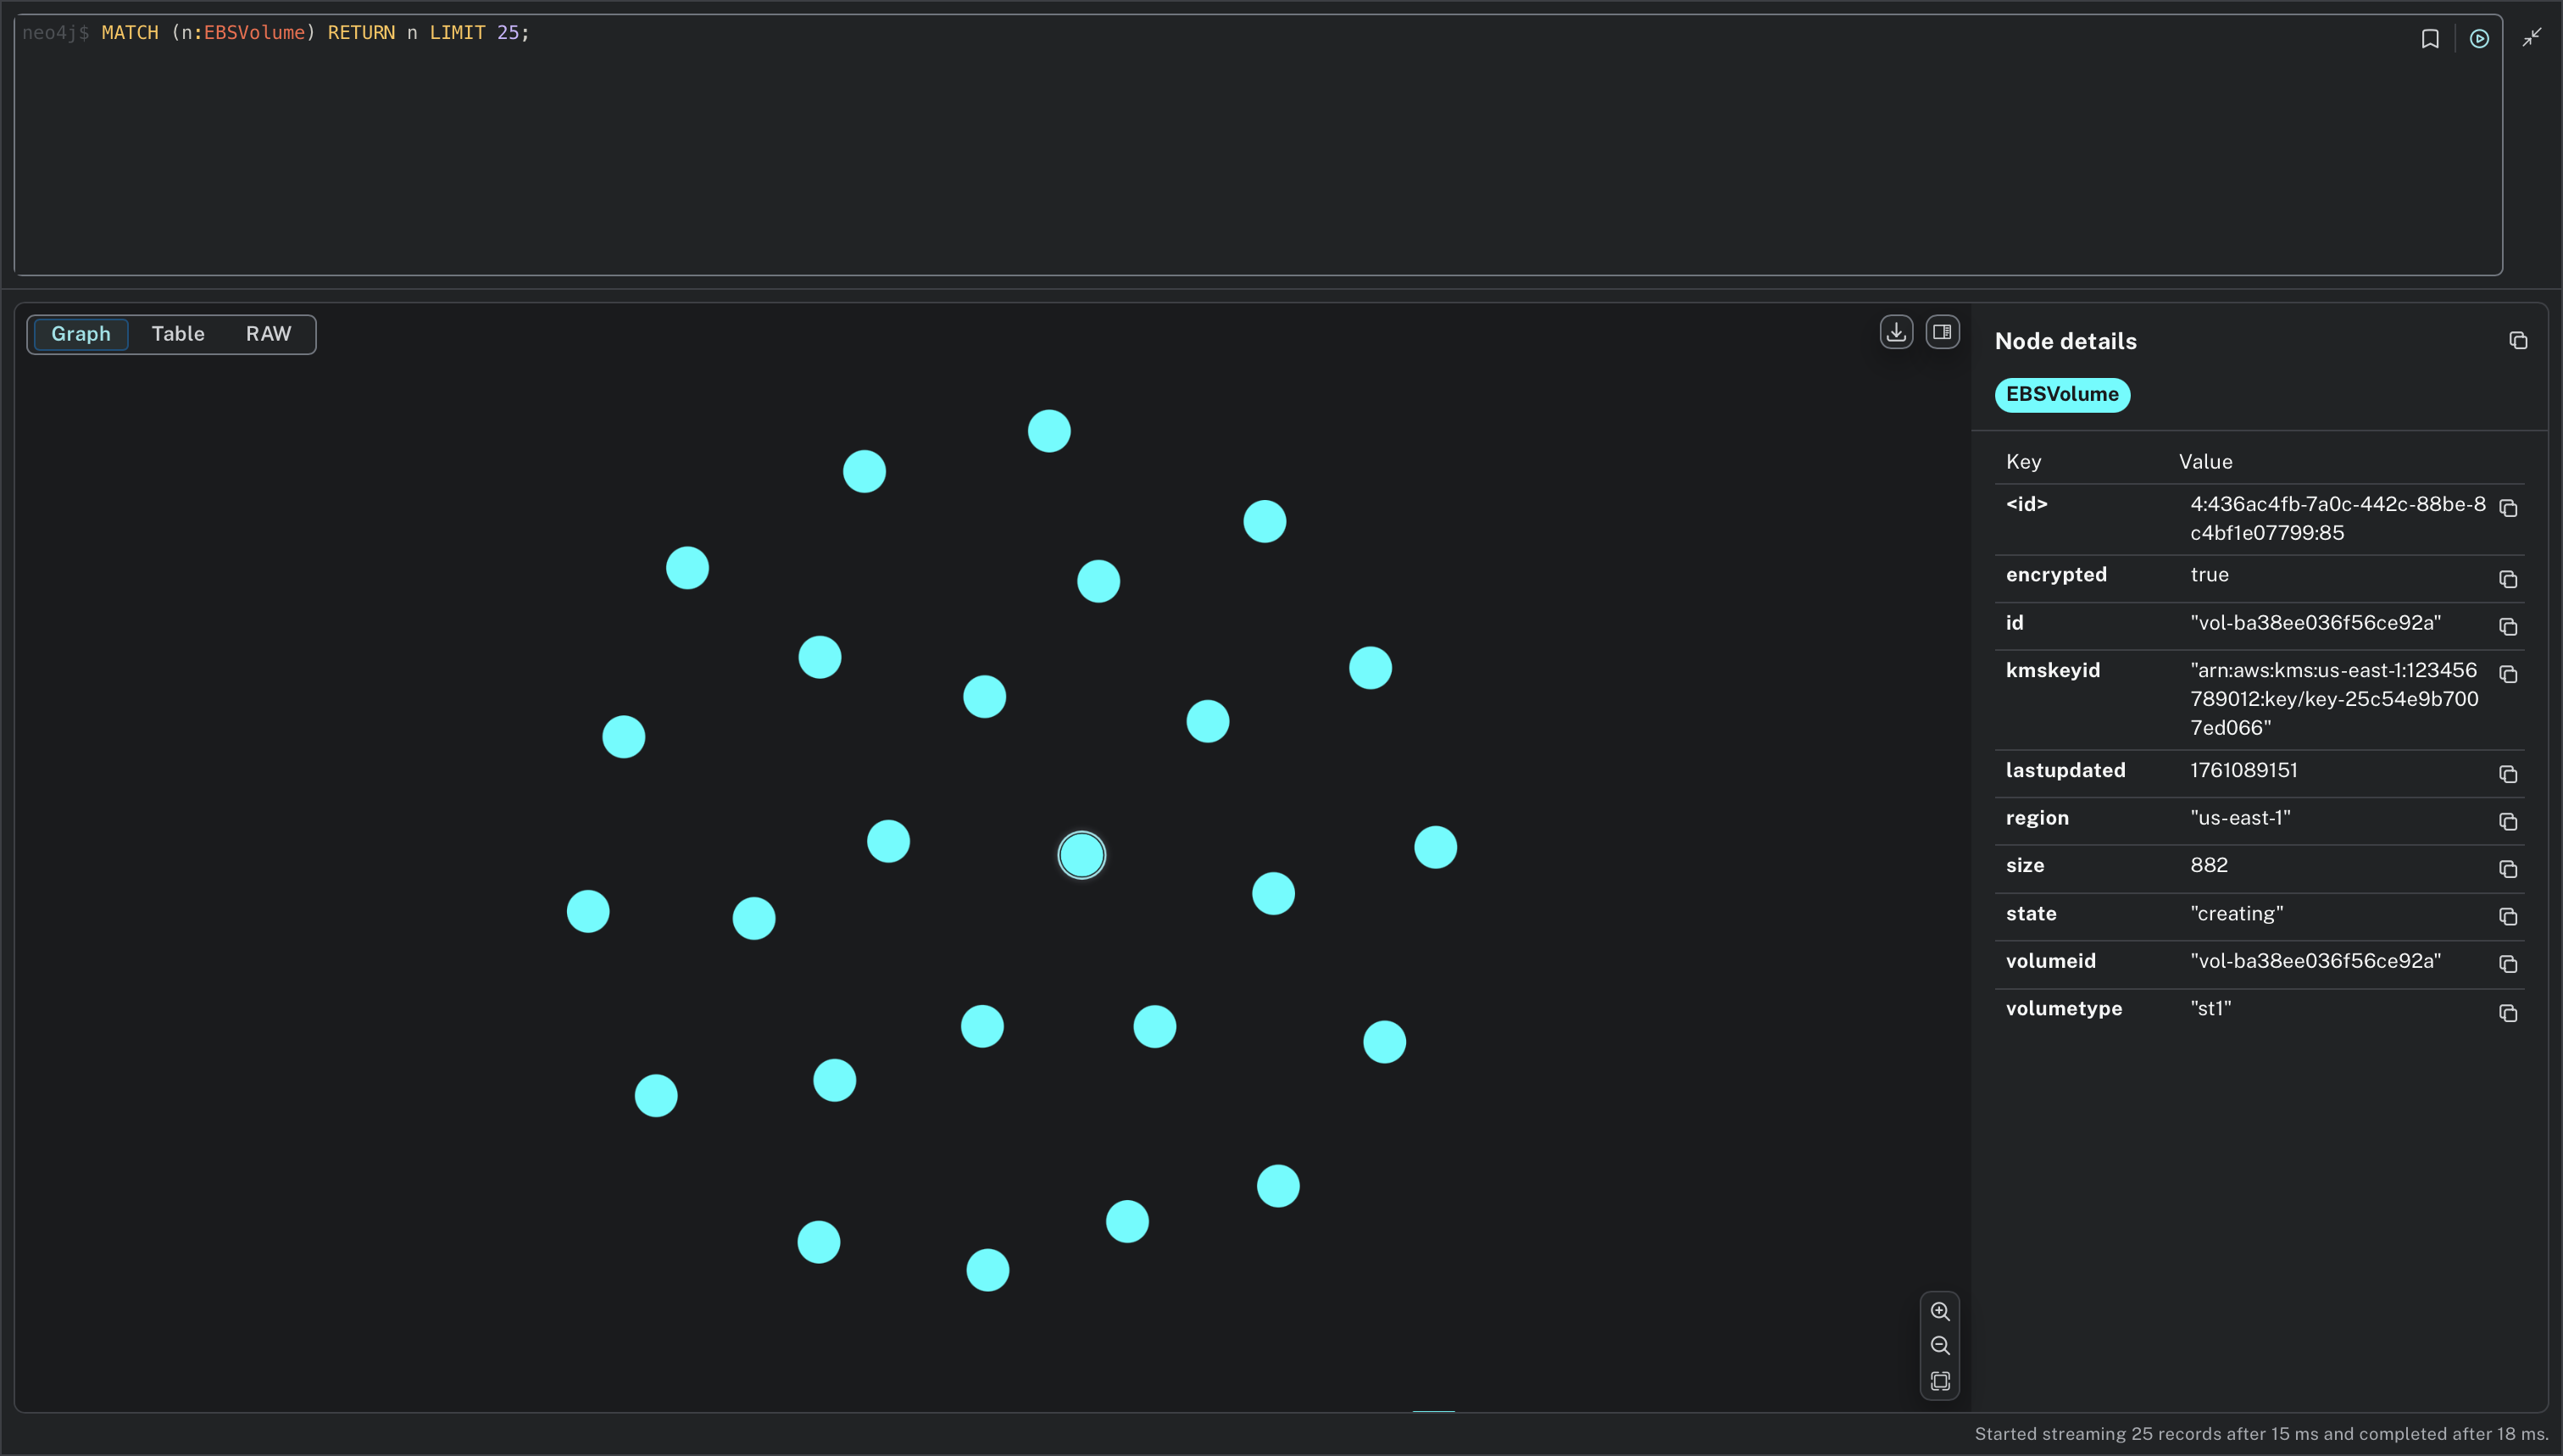
\includegraphics[width=\textwidth]{EBSVolumes.png}
\caption{EBS 磁碟節點}
\label{fig:ebs_nodes}
\end{subfigure}
\hfill
\begin{subfigure}[b]{0.48\textwidth}
\centering
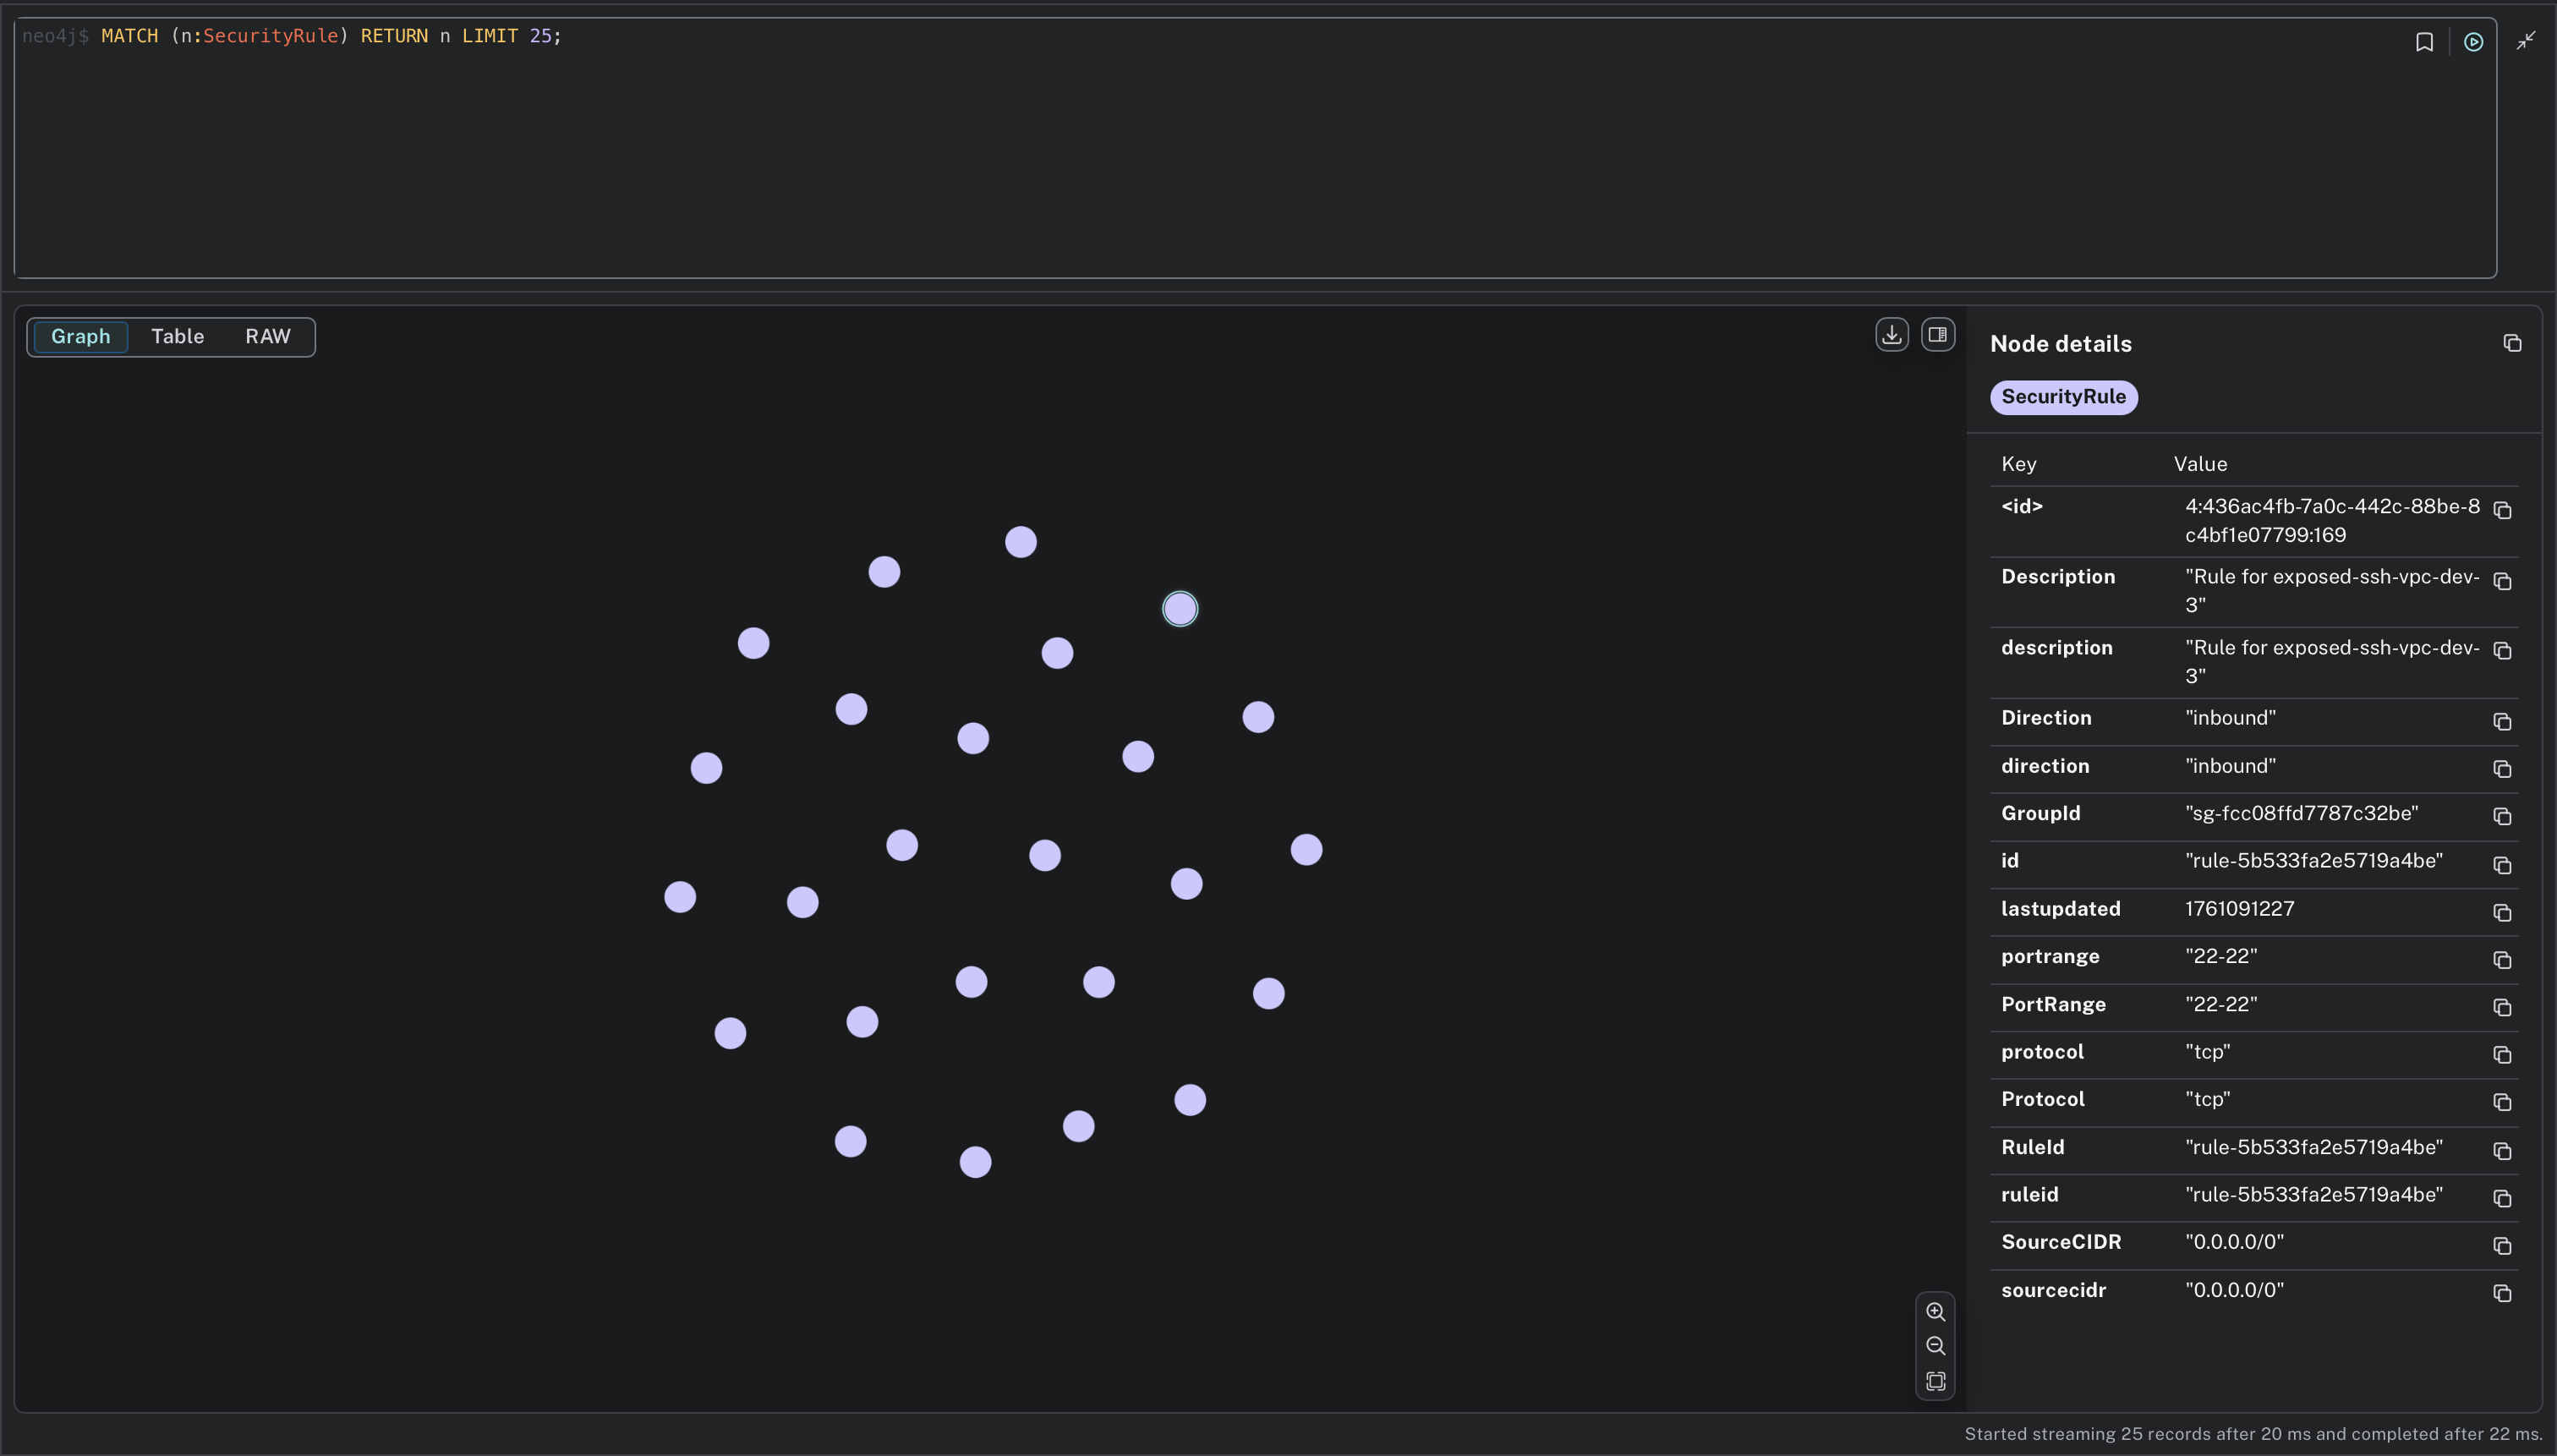
\includegraphics[width=\textwidth]{SecurityRule.png}
\caption{安全規則節點}
\label{fig:rule_nodes}
\end{subfigure}
\caption{儲存和安全規則節點}
\label{fig:storage_security_nodes}
\end{figure}

\subsubsection{關係類型查詢結果}

\begin{figure}[H]
\centering
\begin{subfigure}[b]{0.48\textwidth}
\centering
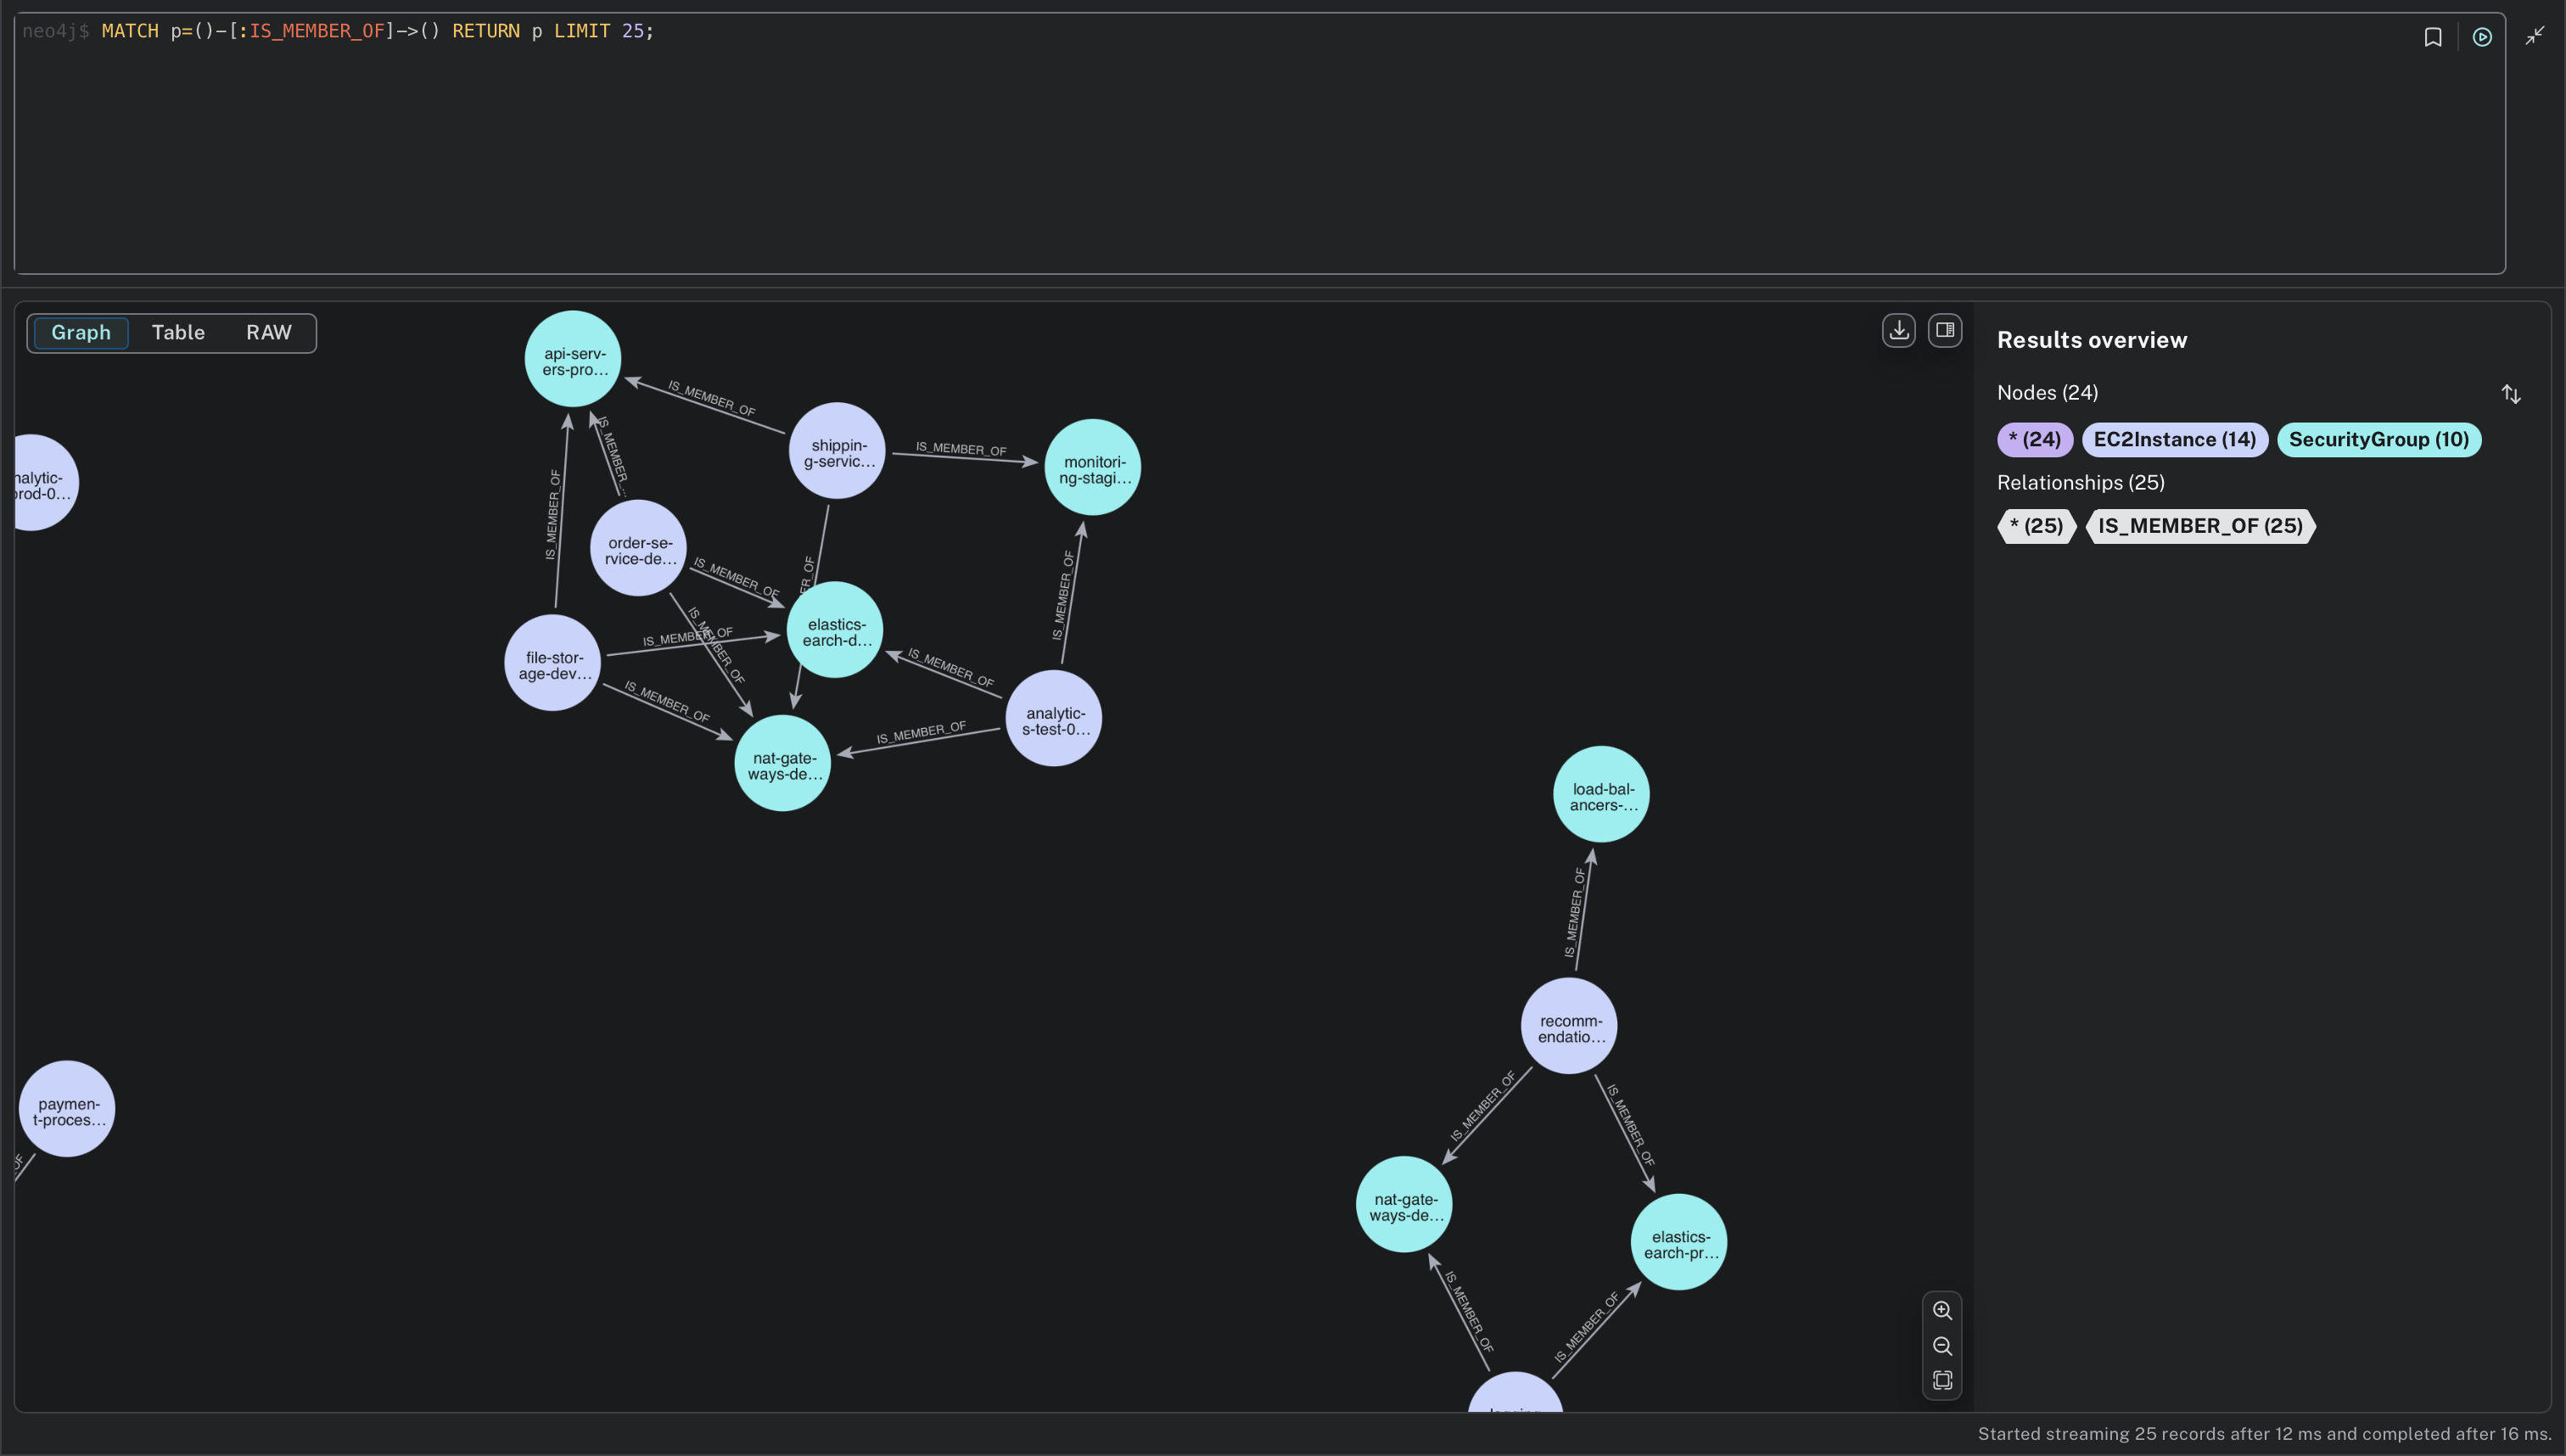
\includegraphics[width=\textwidth]{IS_MEMBER_OF.png}
\caption{IS\_MEMBER\_OF 關係}
\label{fig:is_member_of}
\end{subfigure}
\hfill
\begin{subfigure}[b]{0.48\textwidth}
\centering
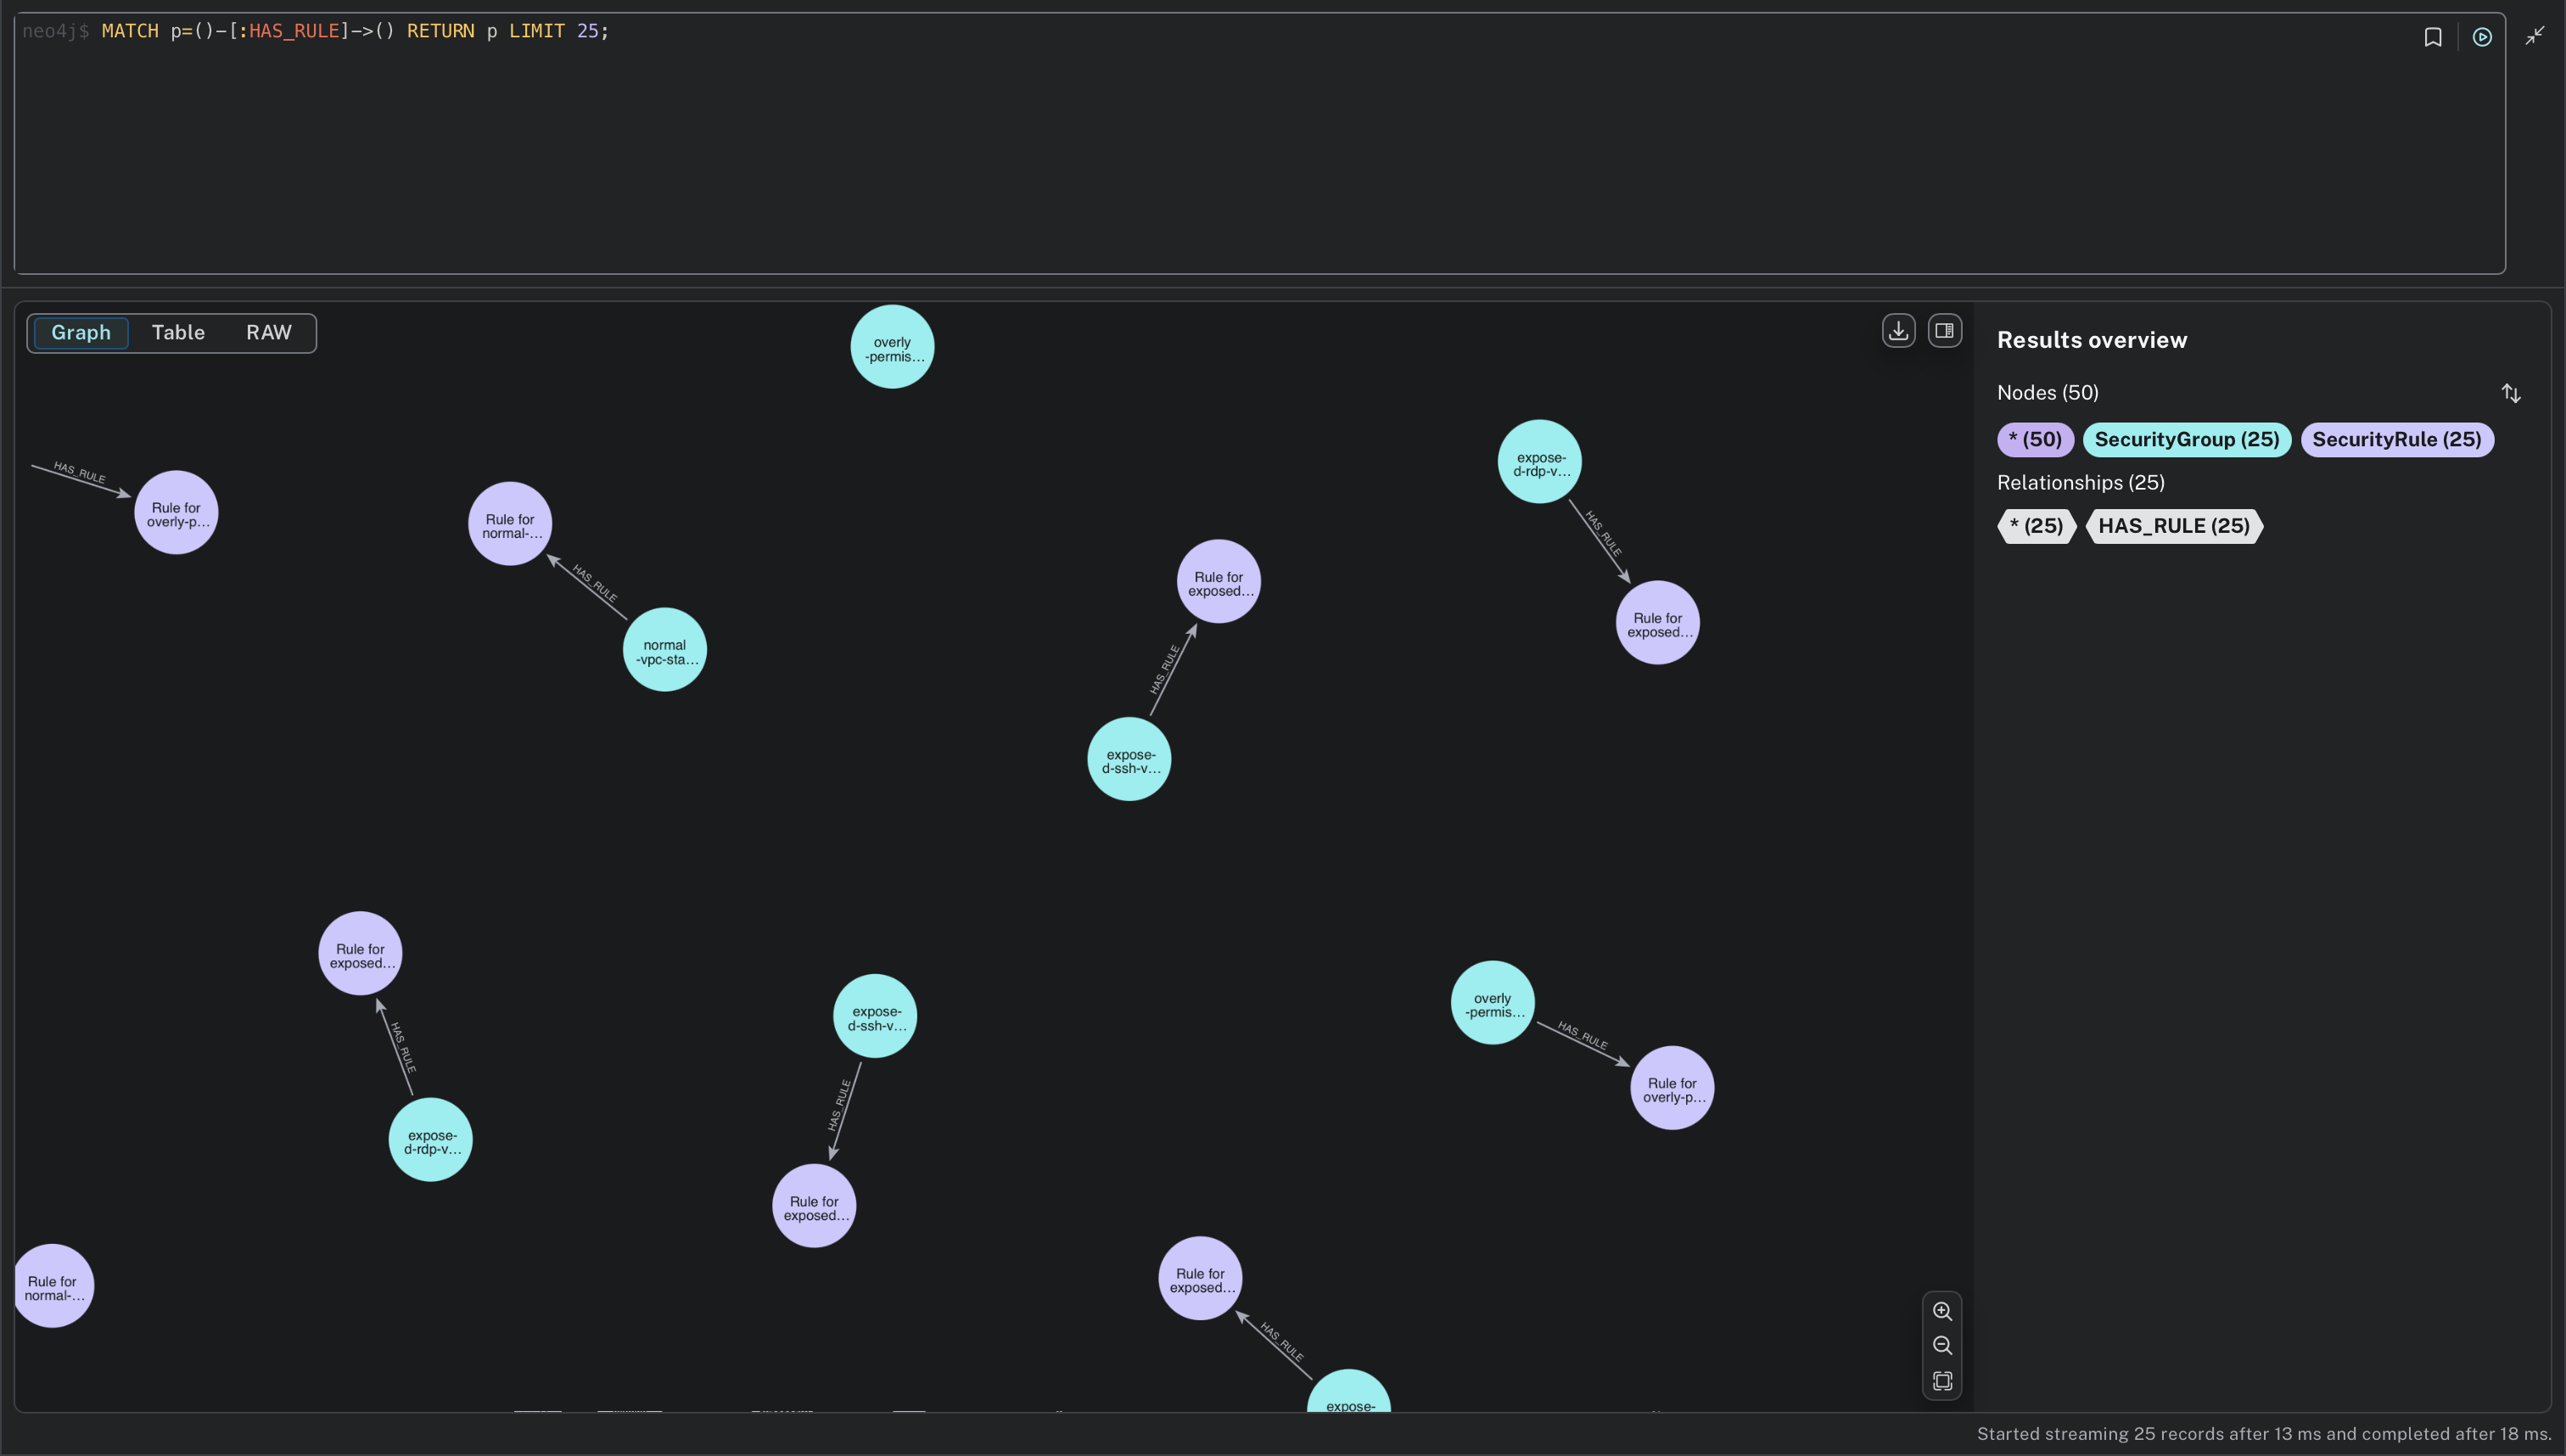
\includegraphics[width=\textwidth]{HAS_RULE.png}
\caption{HAS\_RULE 關係}
\label{fig:has_rule}
\end{subfigure}
\caption{安全群組相關關係}
\label{fig:security_relationships}
\end{figure}

\begin{figure}[H]
\centering
\begin{subfigure}[b]{0.48\textwidth}
\centering
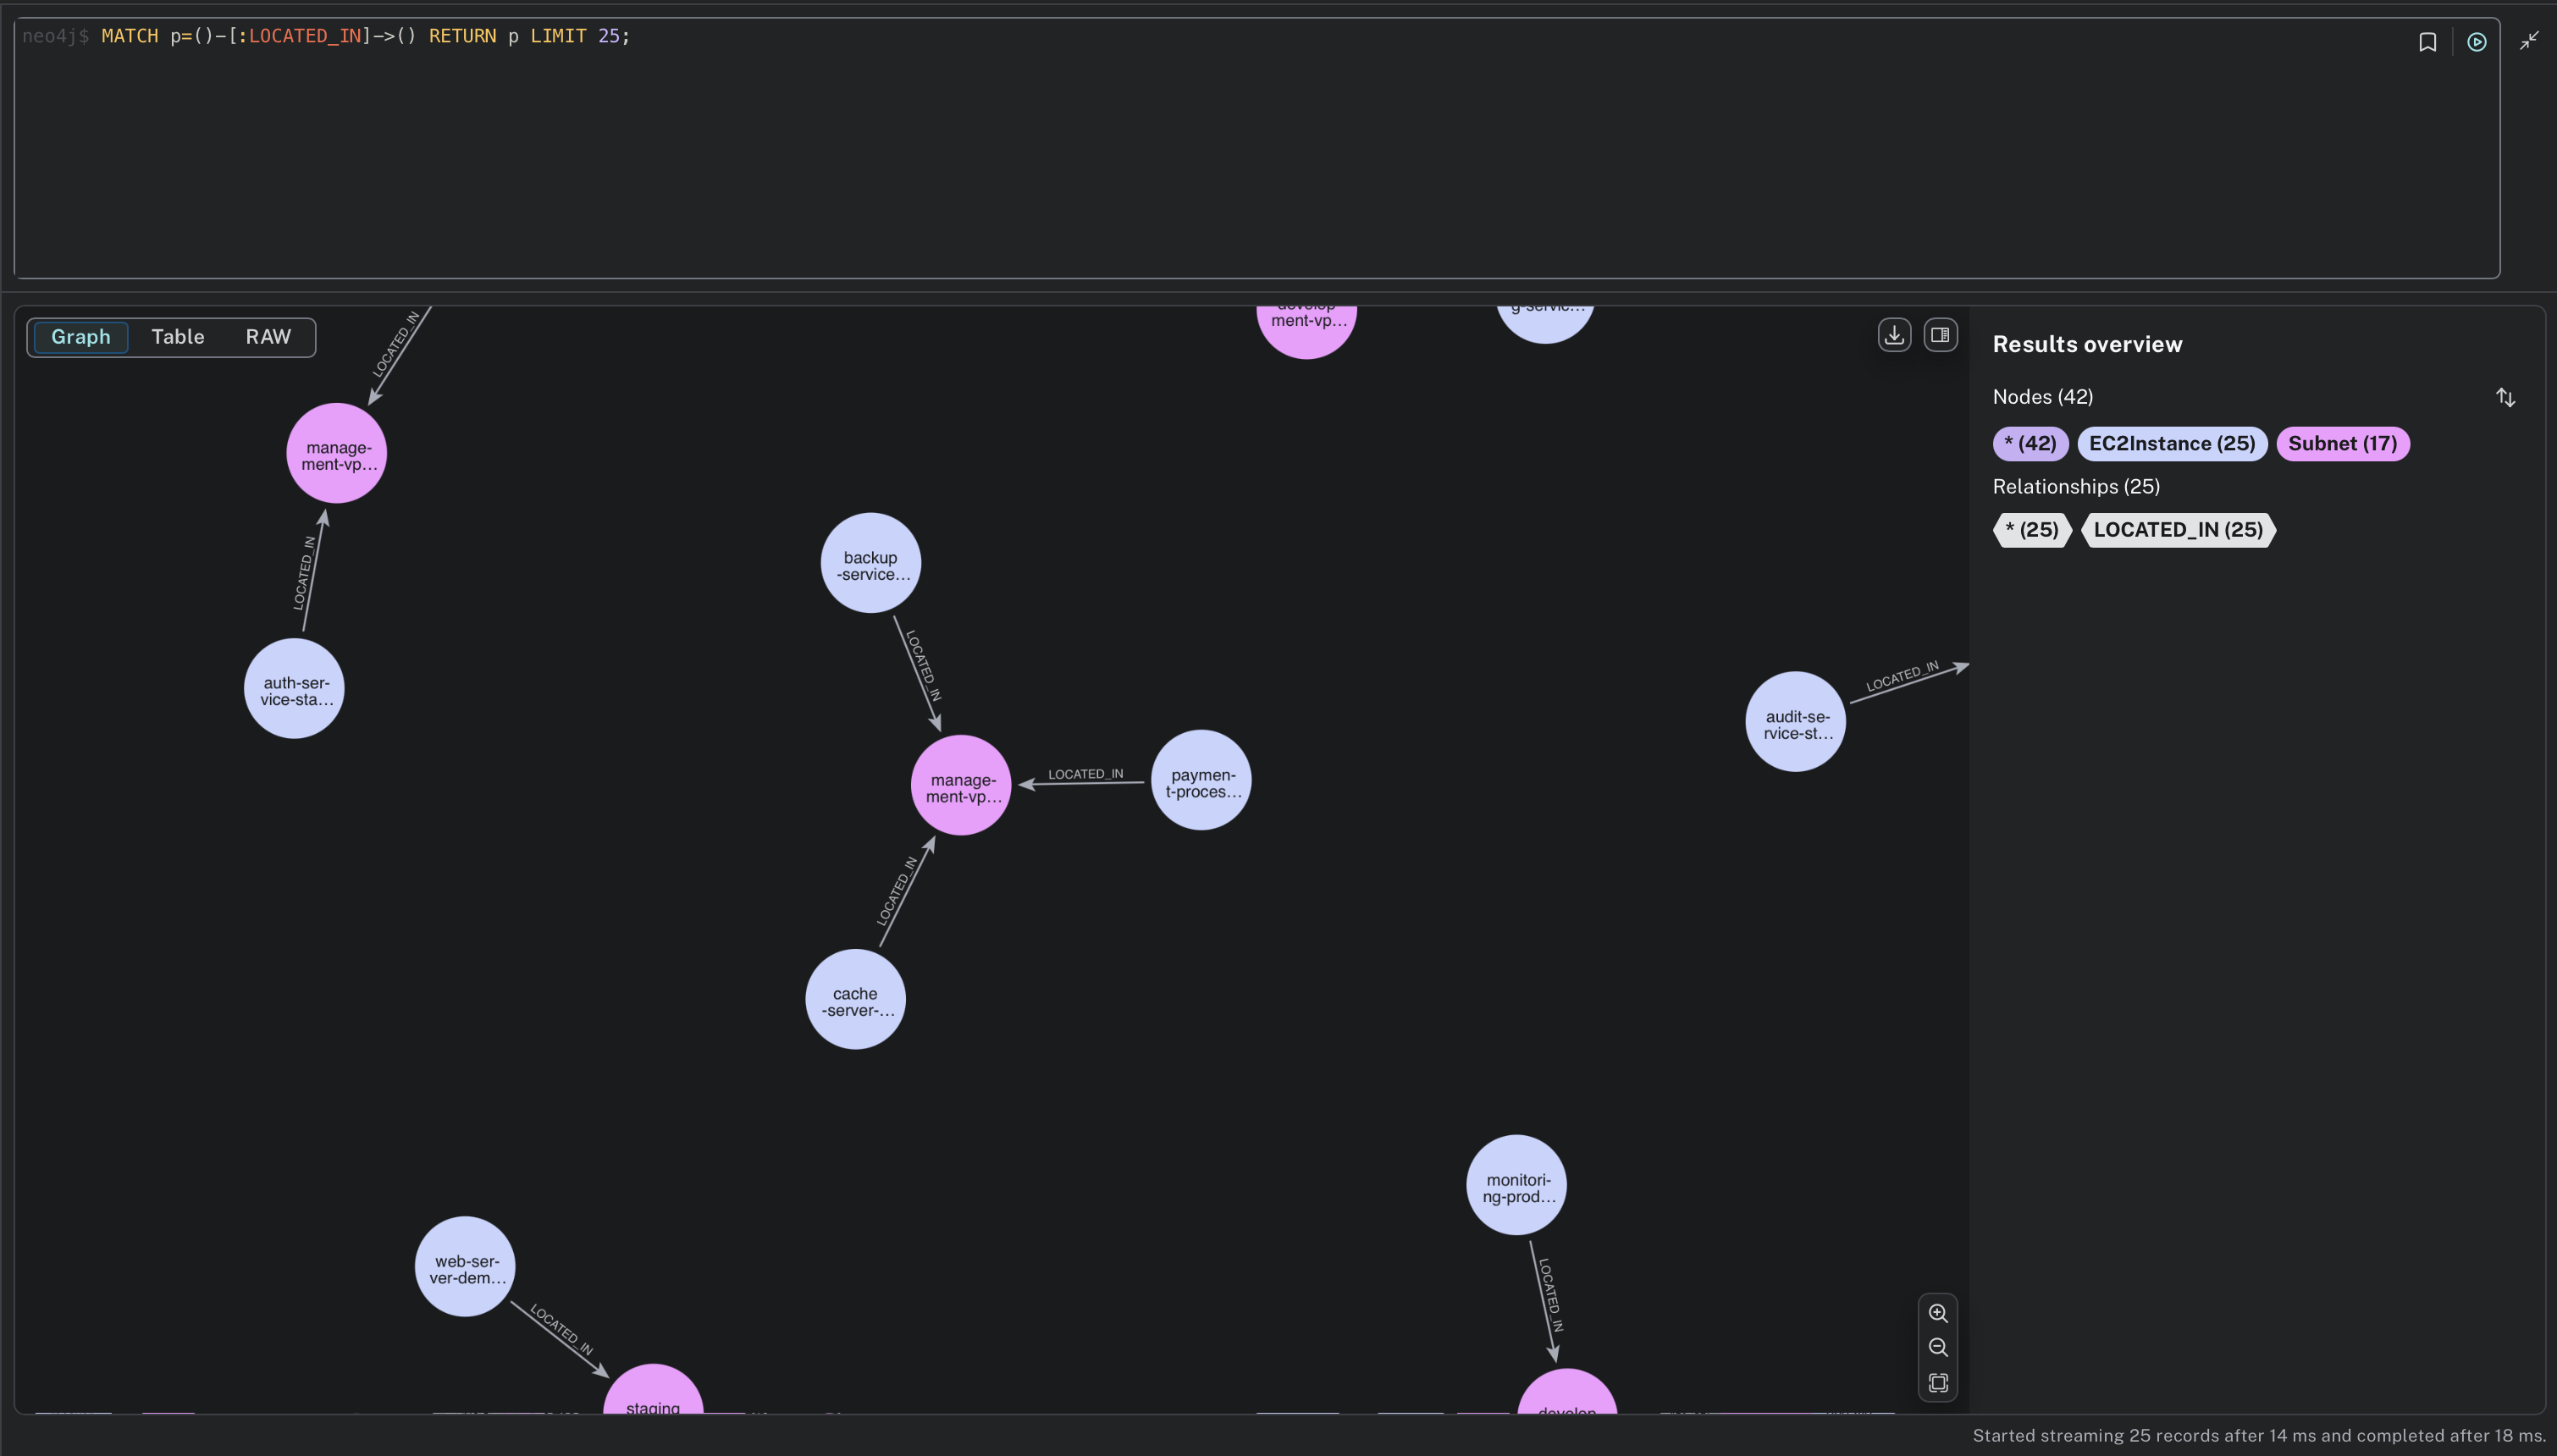
\includegraphics[width=\textwidth]{LOCATED_IN.png}
\caption{LOCATED\_IN 關係}
\label{fig:located_in}
\end{subfigure}
\hfill
\begin{subfigure}[b]{0.48\textwidth}
\centering
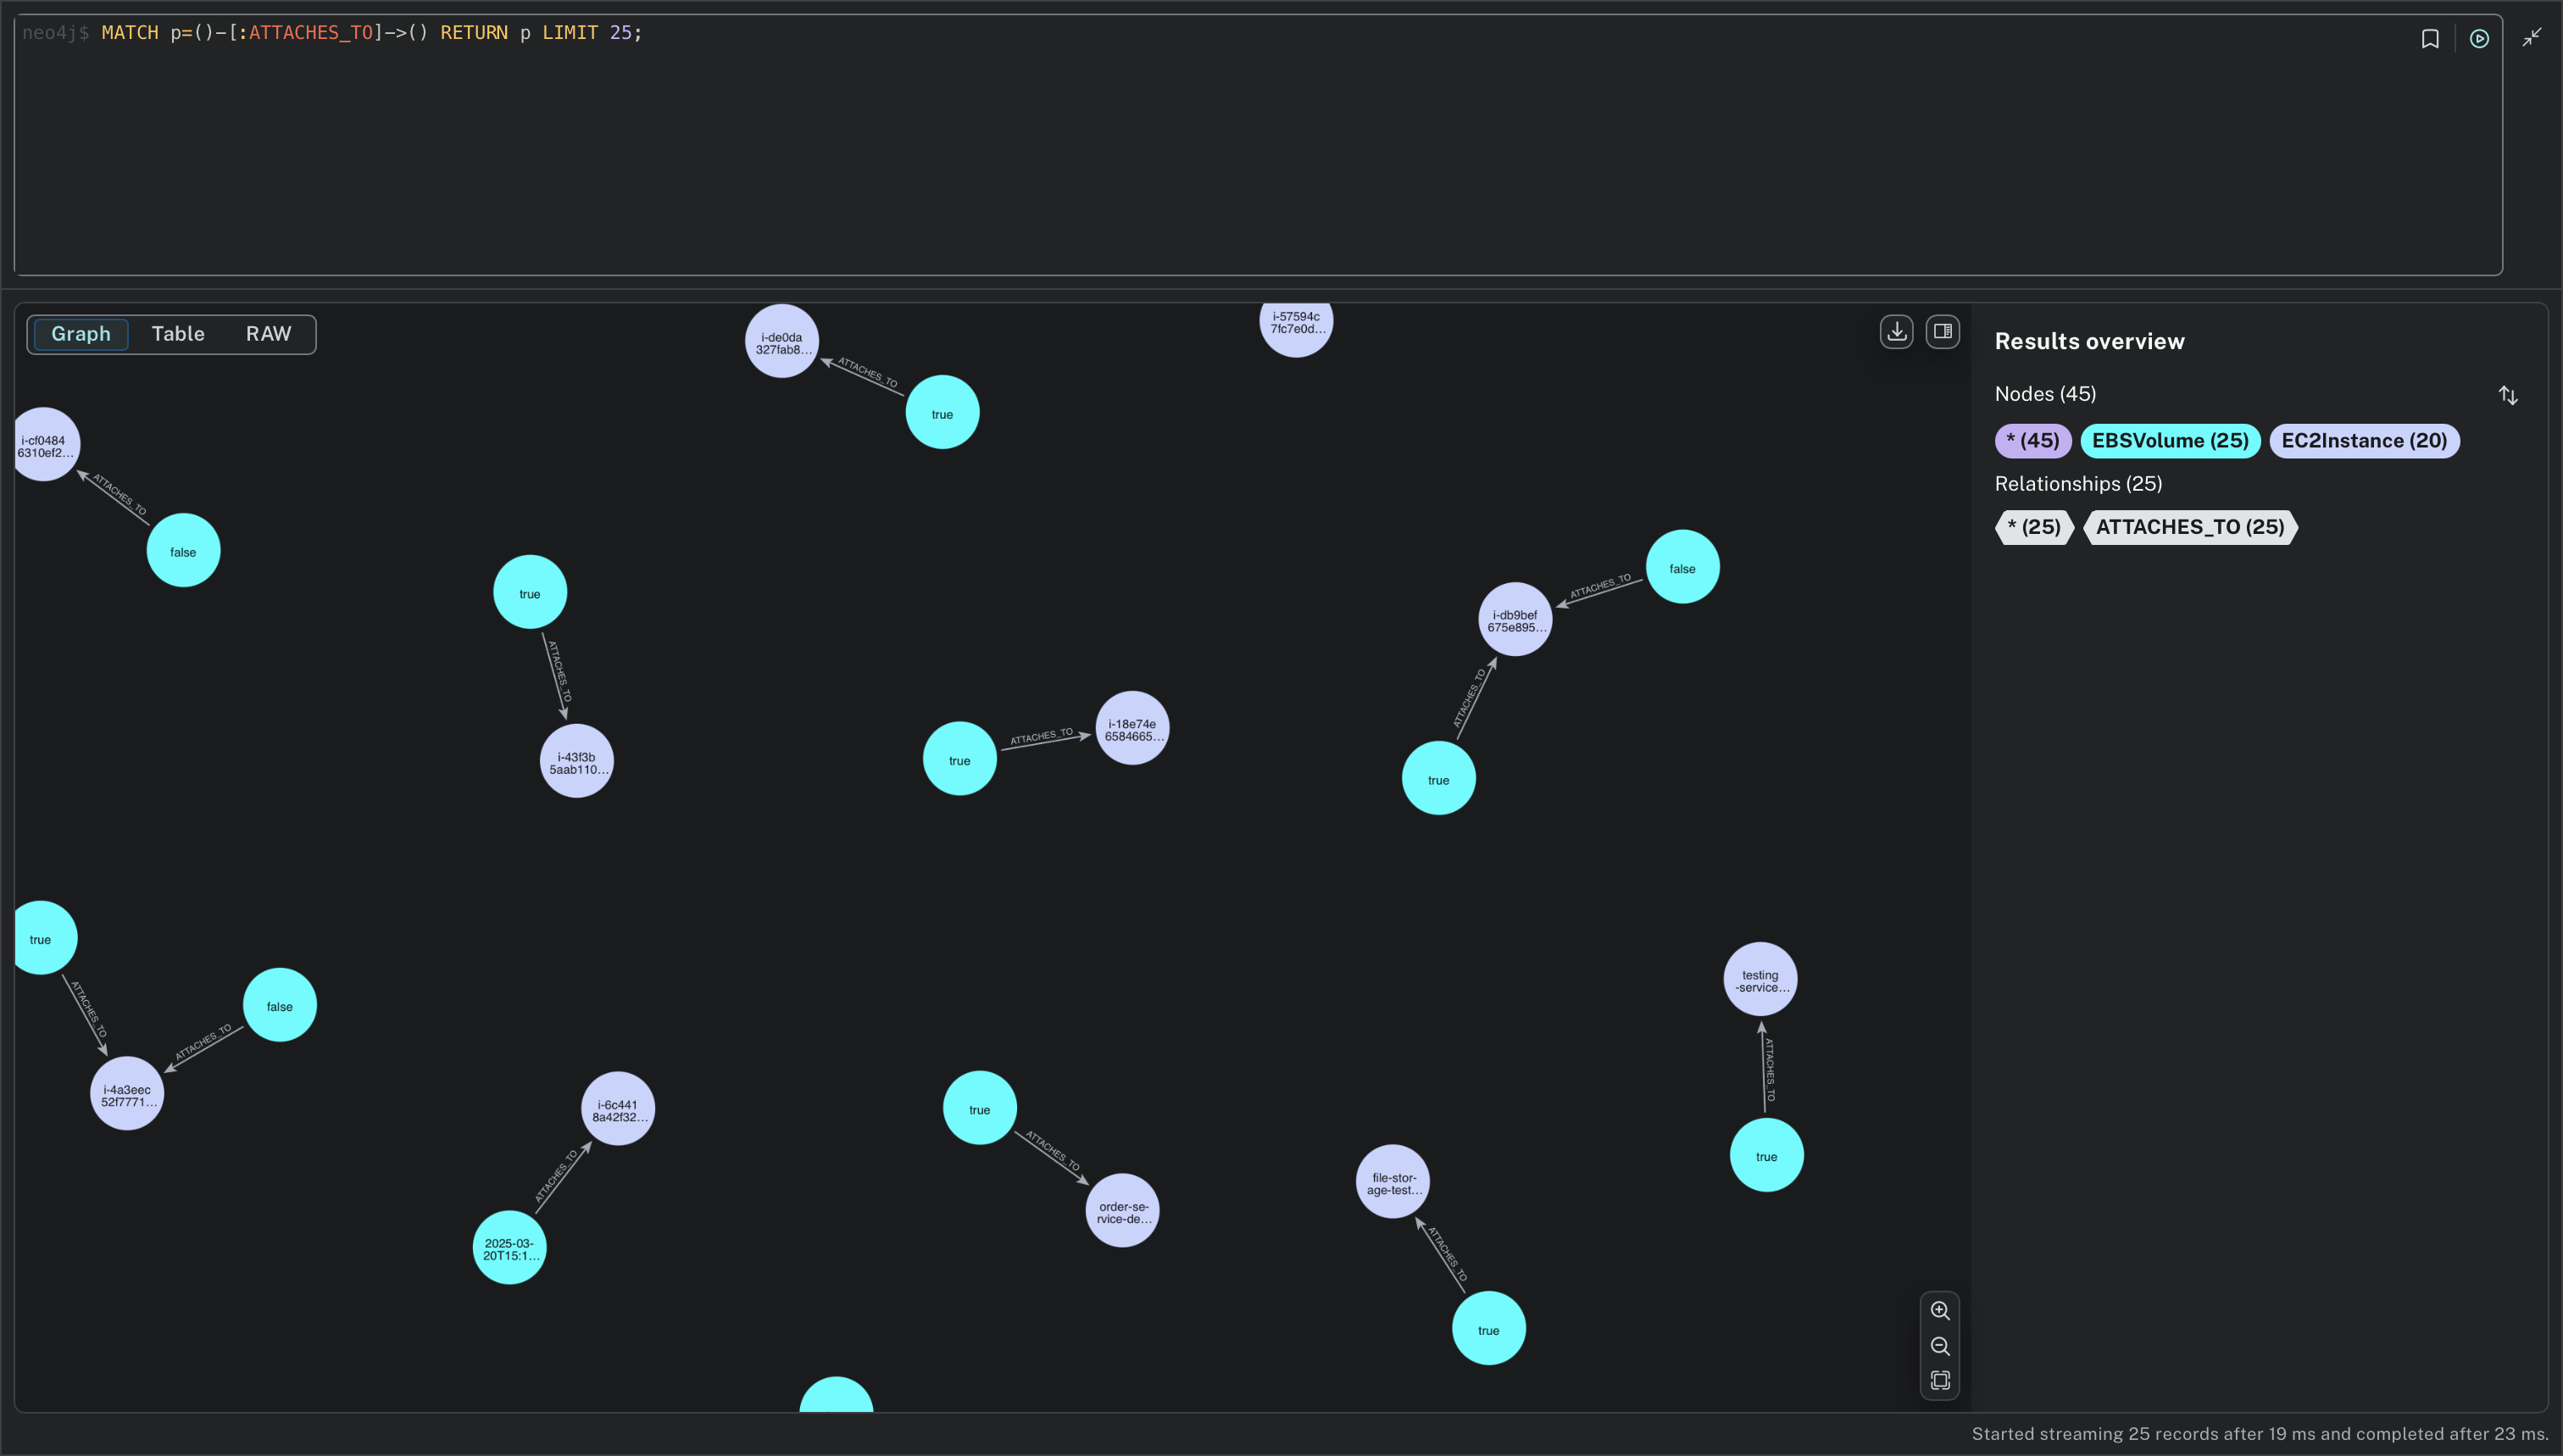
\includegraphics[width=\textwidth]{ATTACHES_TO.png}
\caption{ATTACHES\_TO 關係}
\label{fig:attaches_to}
\end{subfigure}
\caption{位置和掛載關係}
\label{fig:location_attachment_relationships}
\end{figure}

\subsubsection{安全性分析查詢結果}

\begin{figure}[H]
\centering
\begin{subfigure}[b]{0.48\textwidth}
\centering
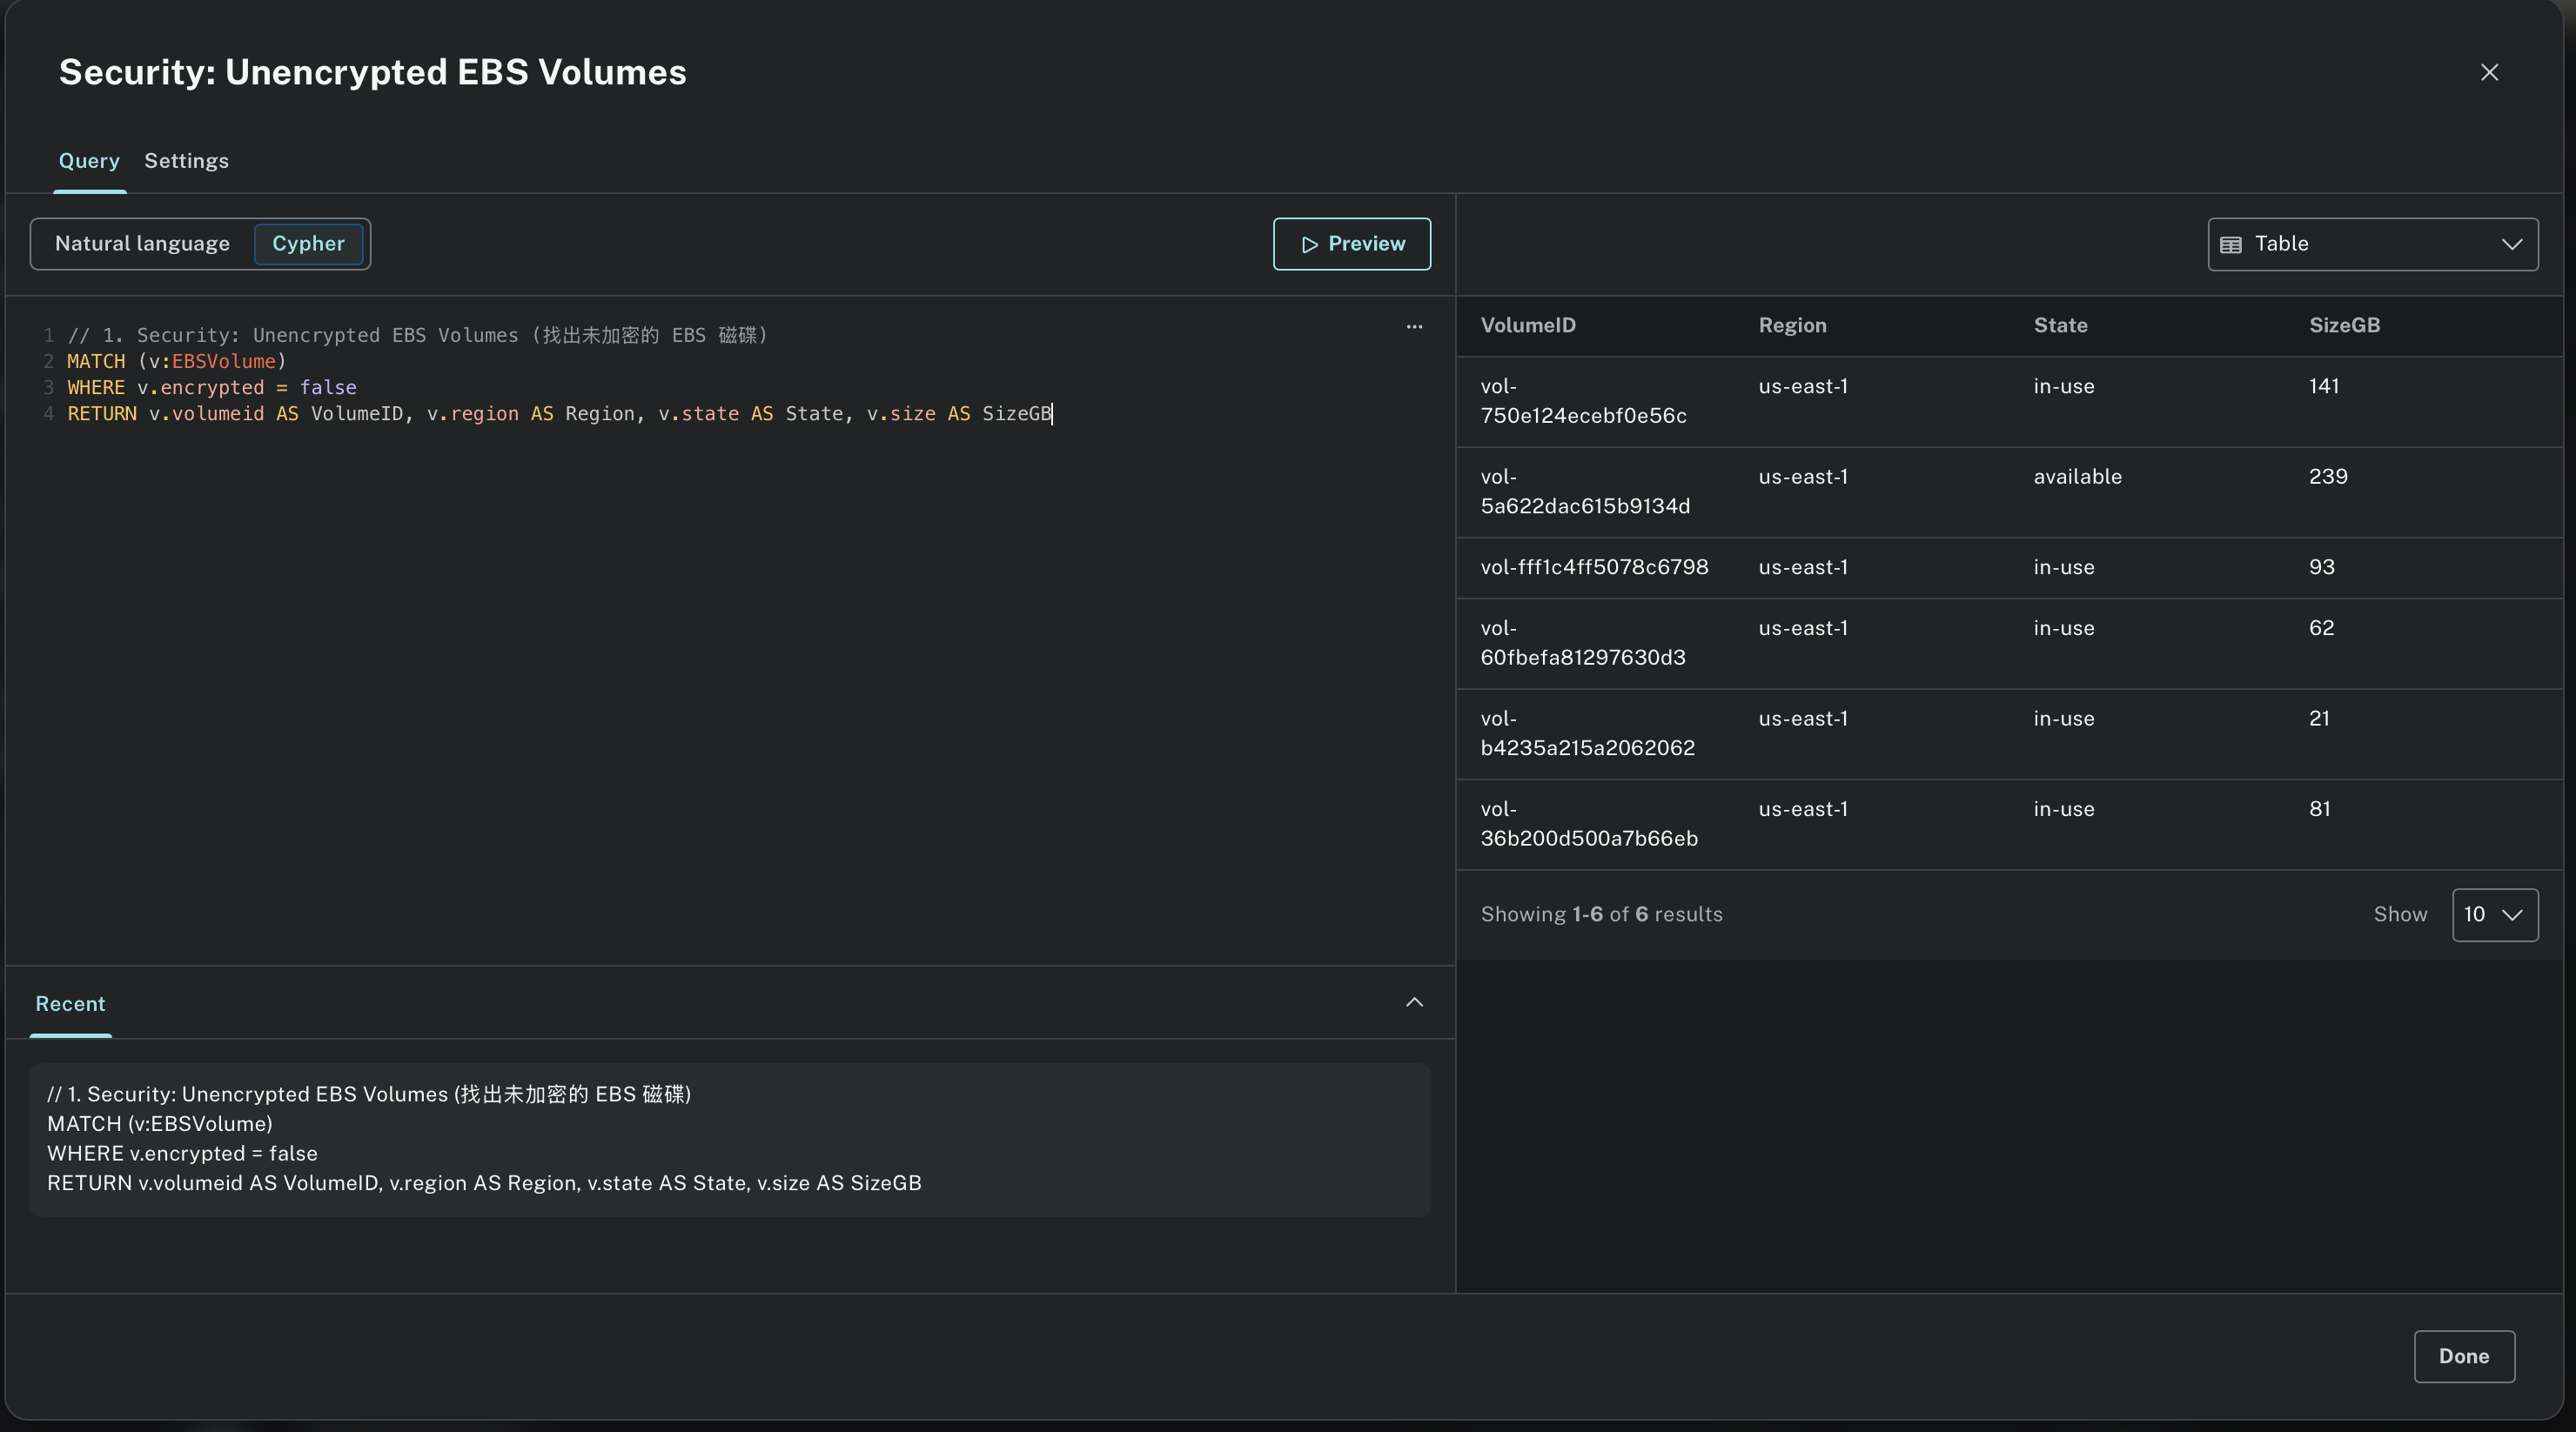
\includegraphics[width=\textwidth]{UnencryptedEBSVolumes.png}
\caption{未加密 EBS 磁碟檢測}
\label{fig:unencrypted_ebs}
\end{subfigure}
\hfill
\begin{subfigure}[b]{0.48\textwidth}
\centering
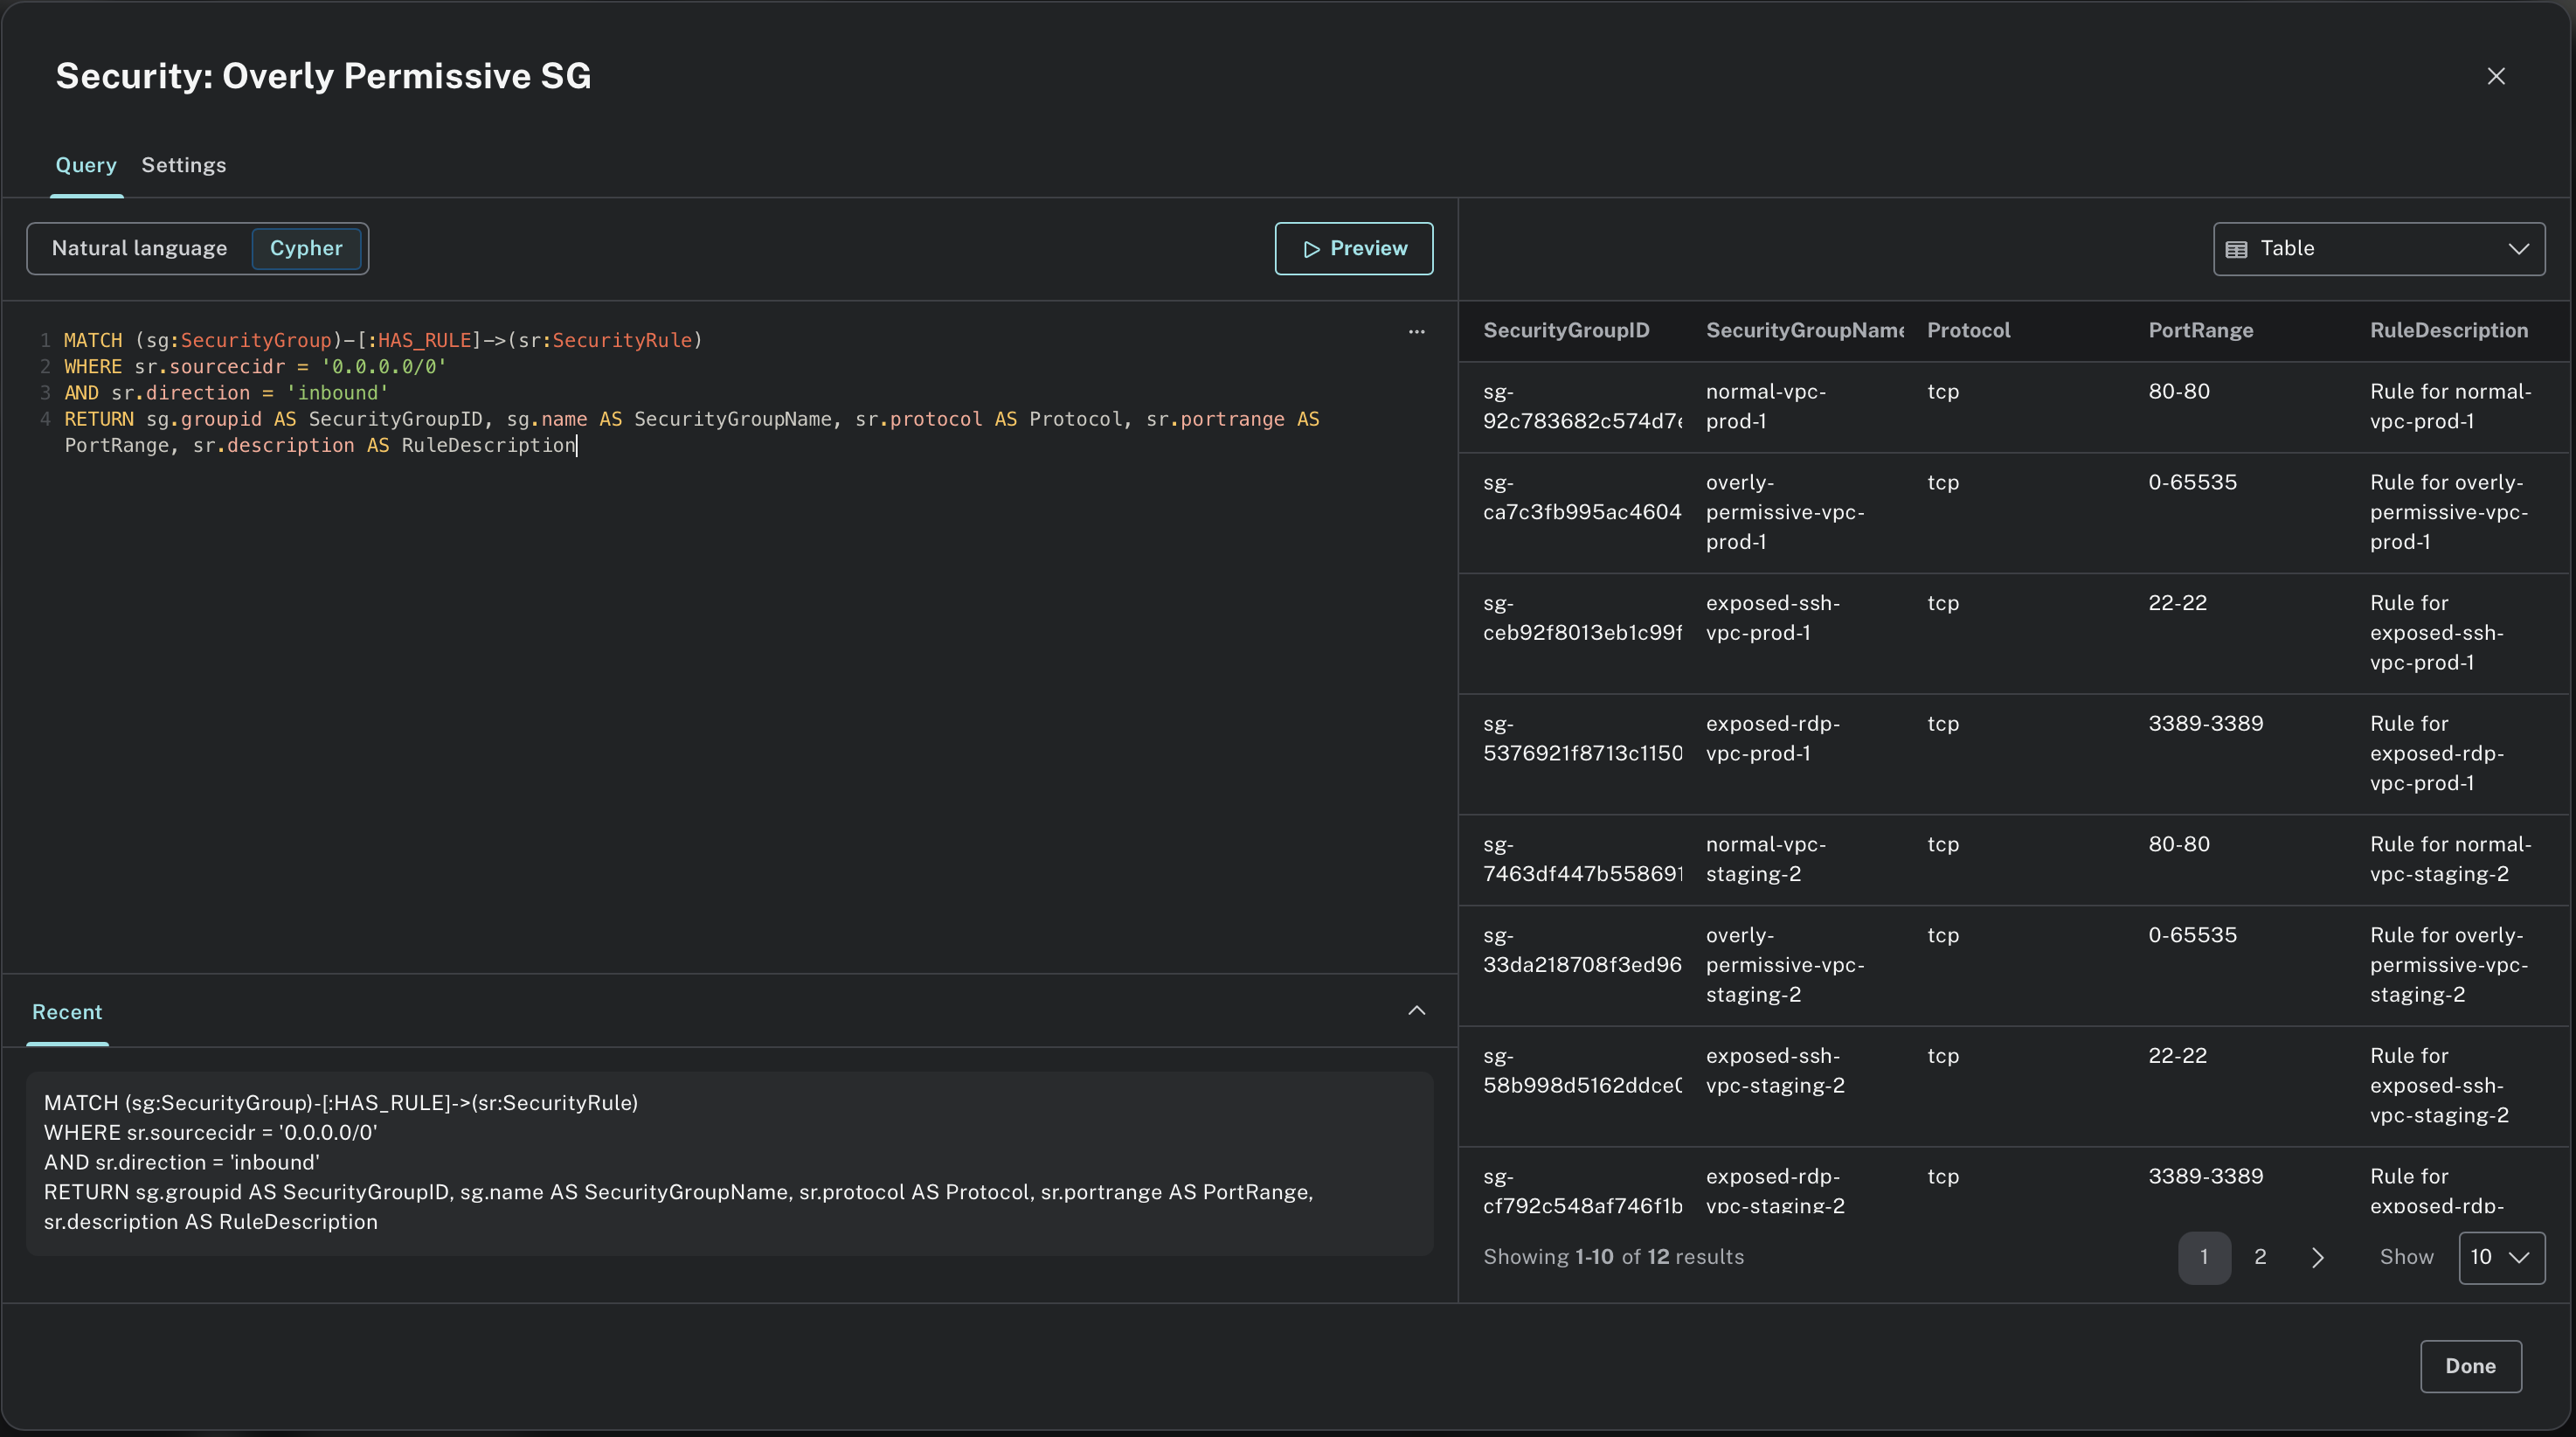
\includegraphics[width=\textwidth]{Overly Permissive SG.png}
\caption{過度寬鬆的安全群組檢測}
\label{fig:permissive_sg}
\end{subfigure}
\caption{安全性分析查詢結果}
\label{fig:security_analysis_results}
\end{figure}

\subsubsection{成本優化分析查詢結果}

\begin{figure}[H]
\centering
\begin{subfigure}[b]{0.48\textwidth}
\centering
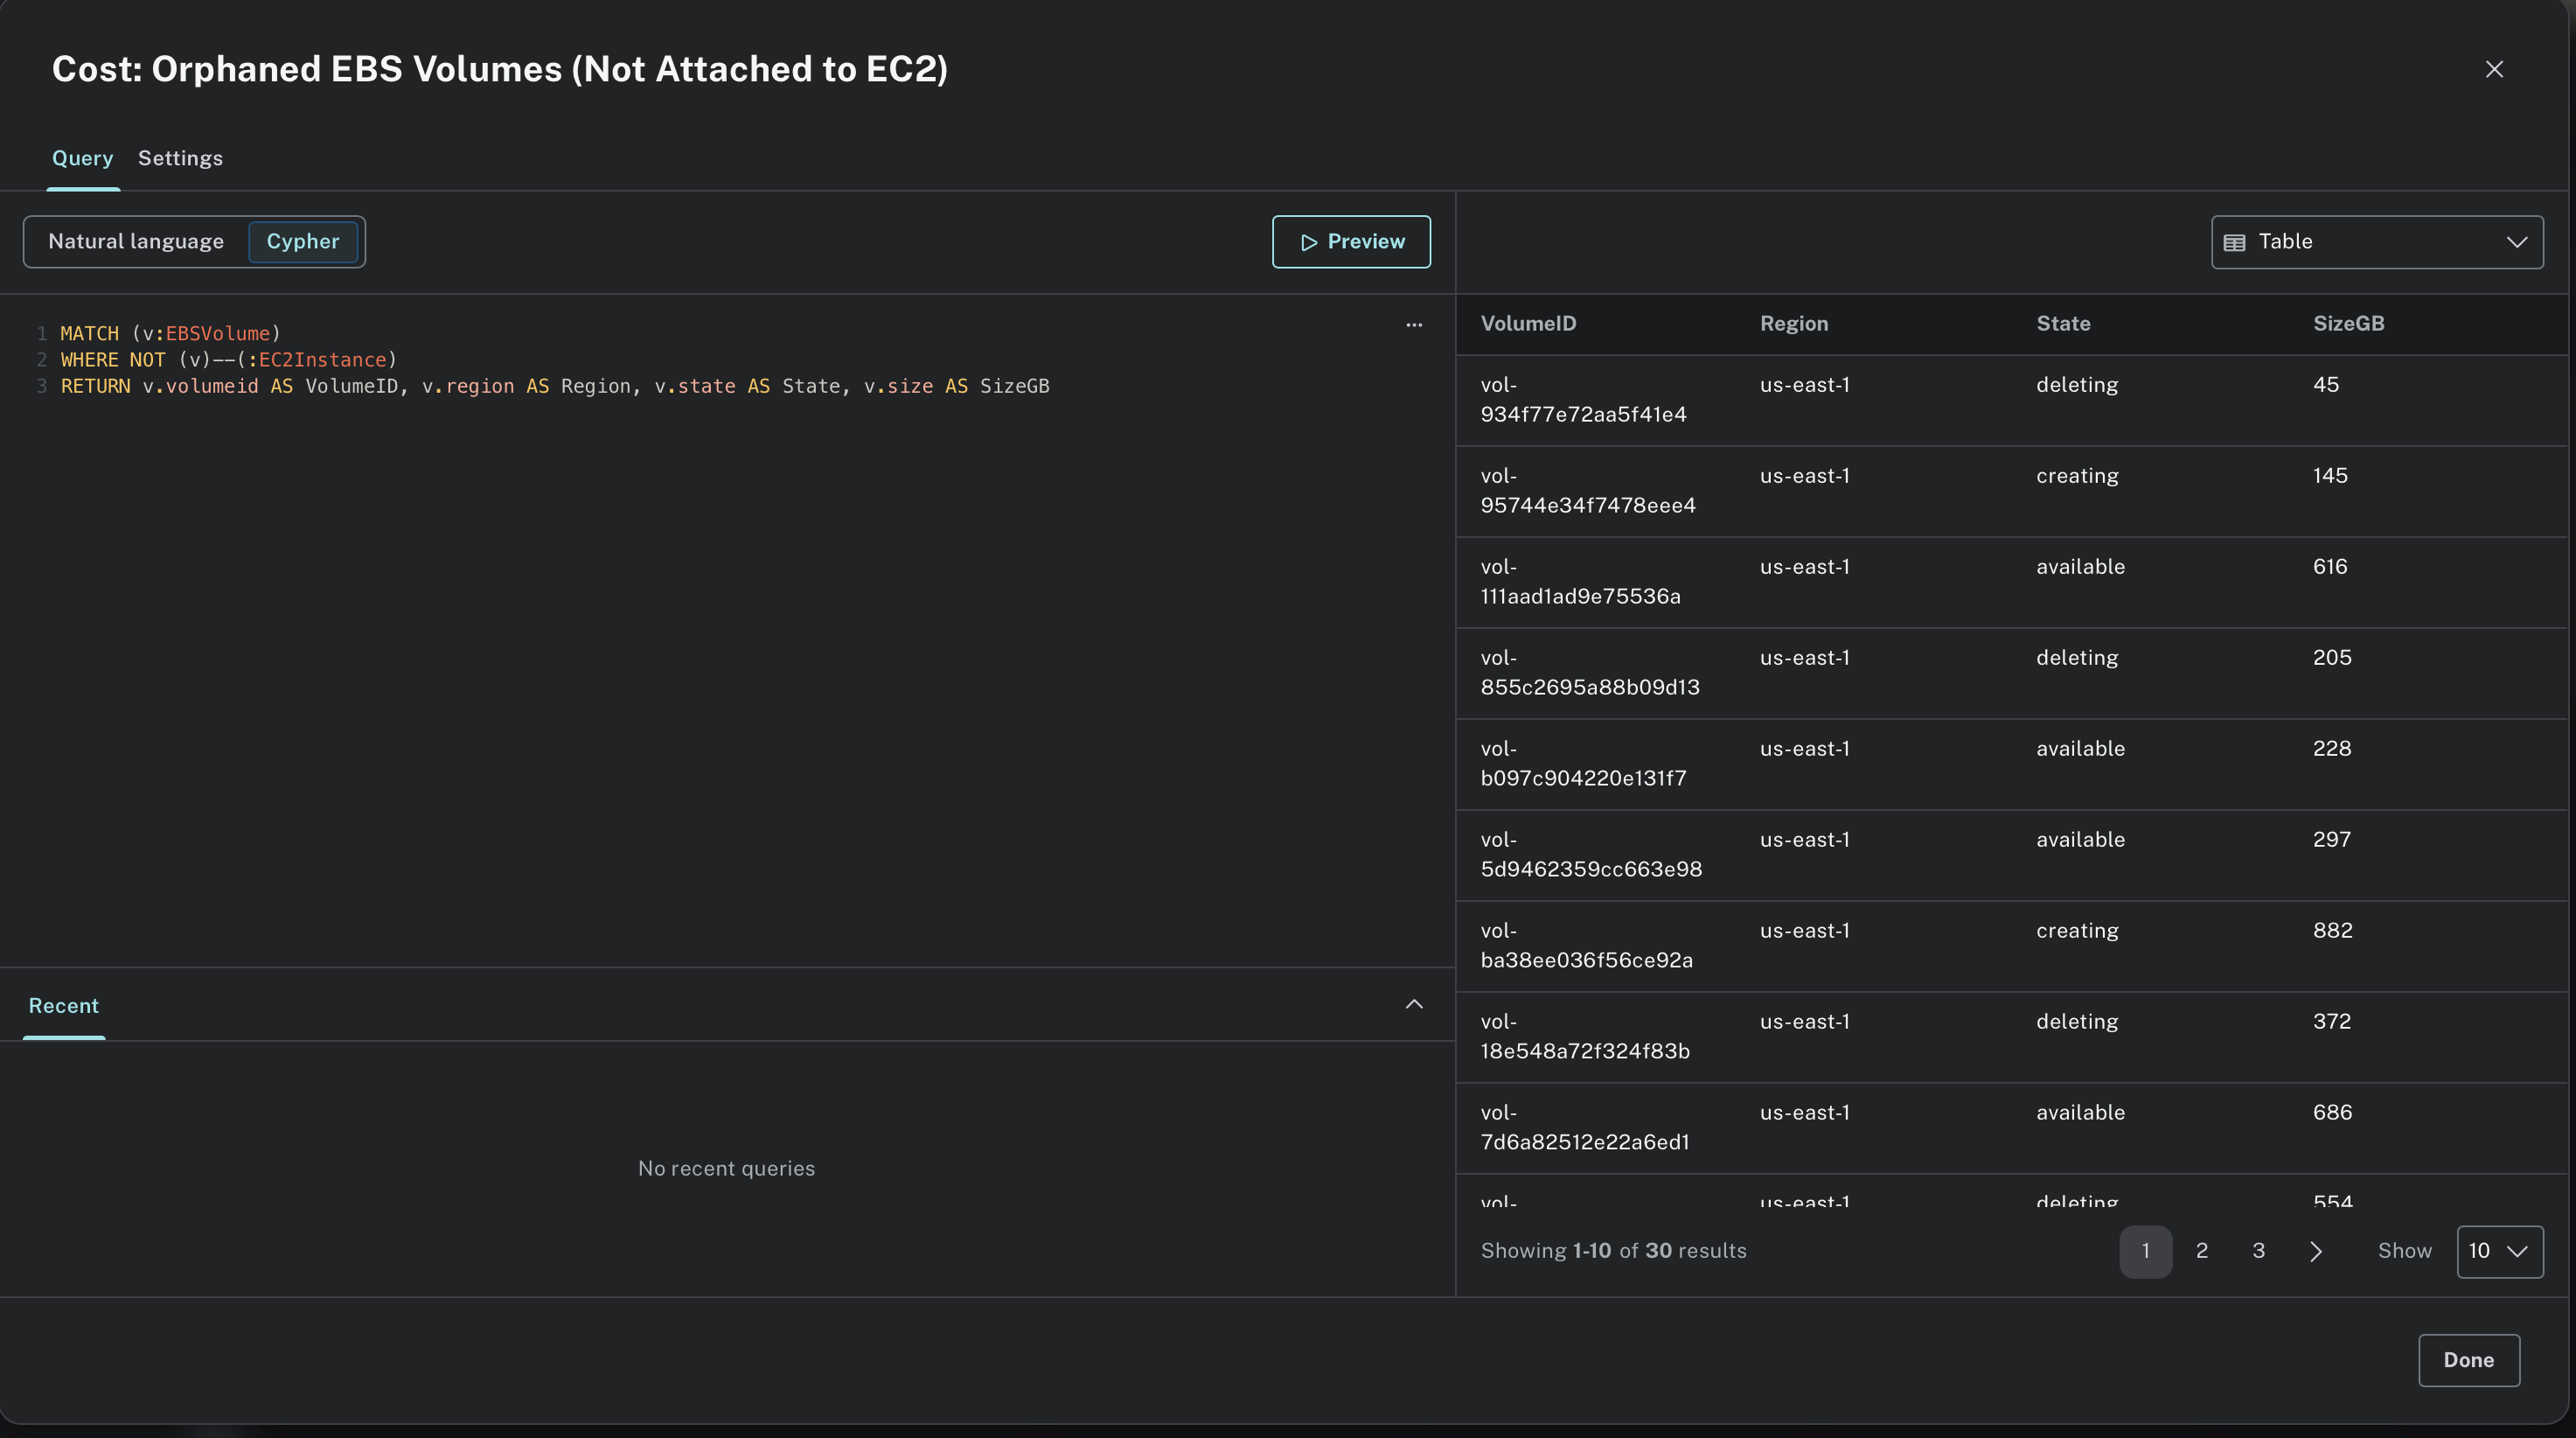
\includegraphics[width=\textwidth]{Orphaned EBS Volumes.png}
\caption{孤兒 EBS 磁碟檢測}
\label{fig:orphaned_ebs}
\end{subfigure}
\hfill
\begin{subfigure}[b]{0.48\textwidth}
\centering
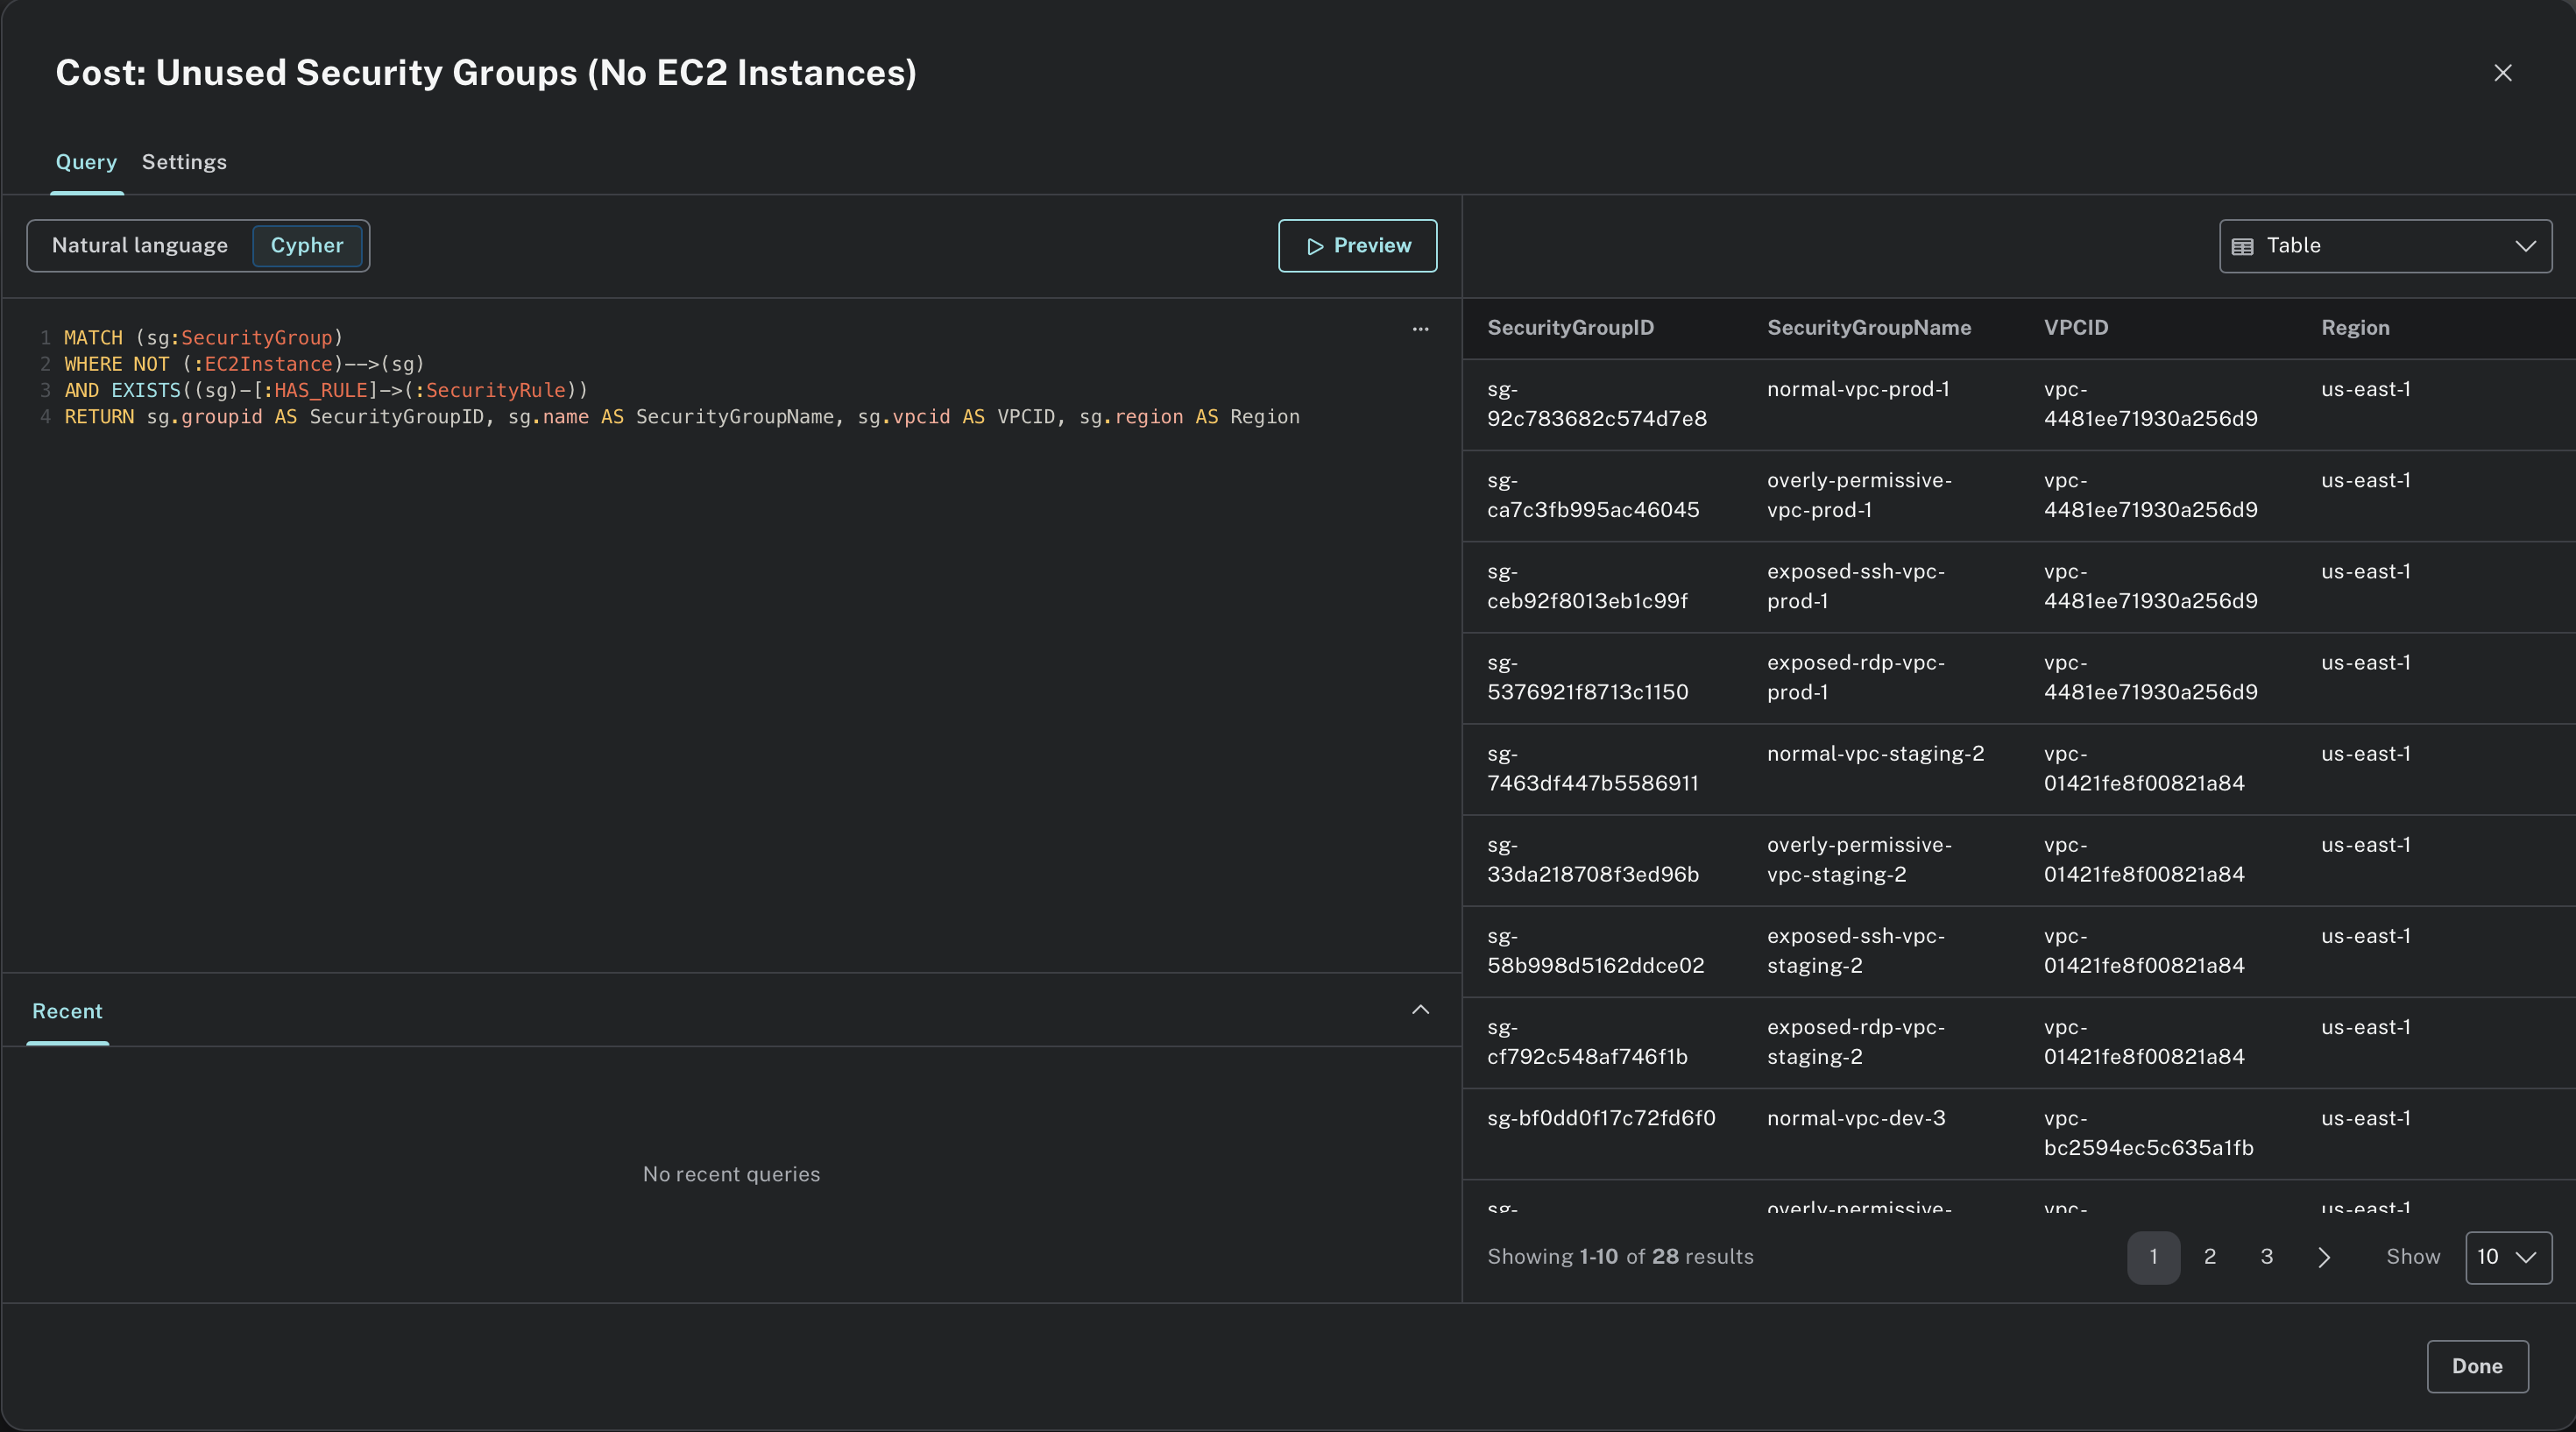
\includegraphics[width=\textwidth]{Unused Security Groups.png}
\caption{未使用的安全群組檢測}
\label{fig:unused_sg}
\end{subfigure}
\caption{成本優化分析查詢結果}
\label{fig:cost_analysis_results}
\end{figure}

\begin{figure}[H]
\centering
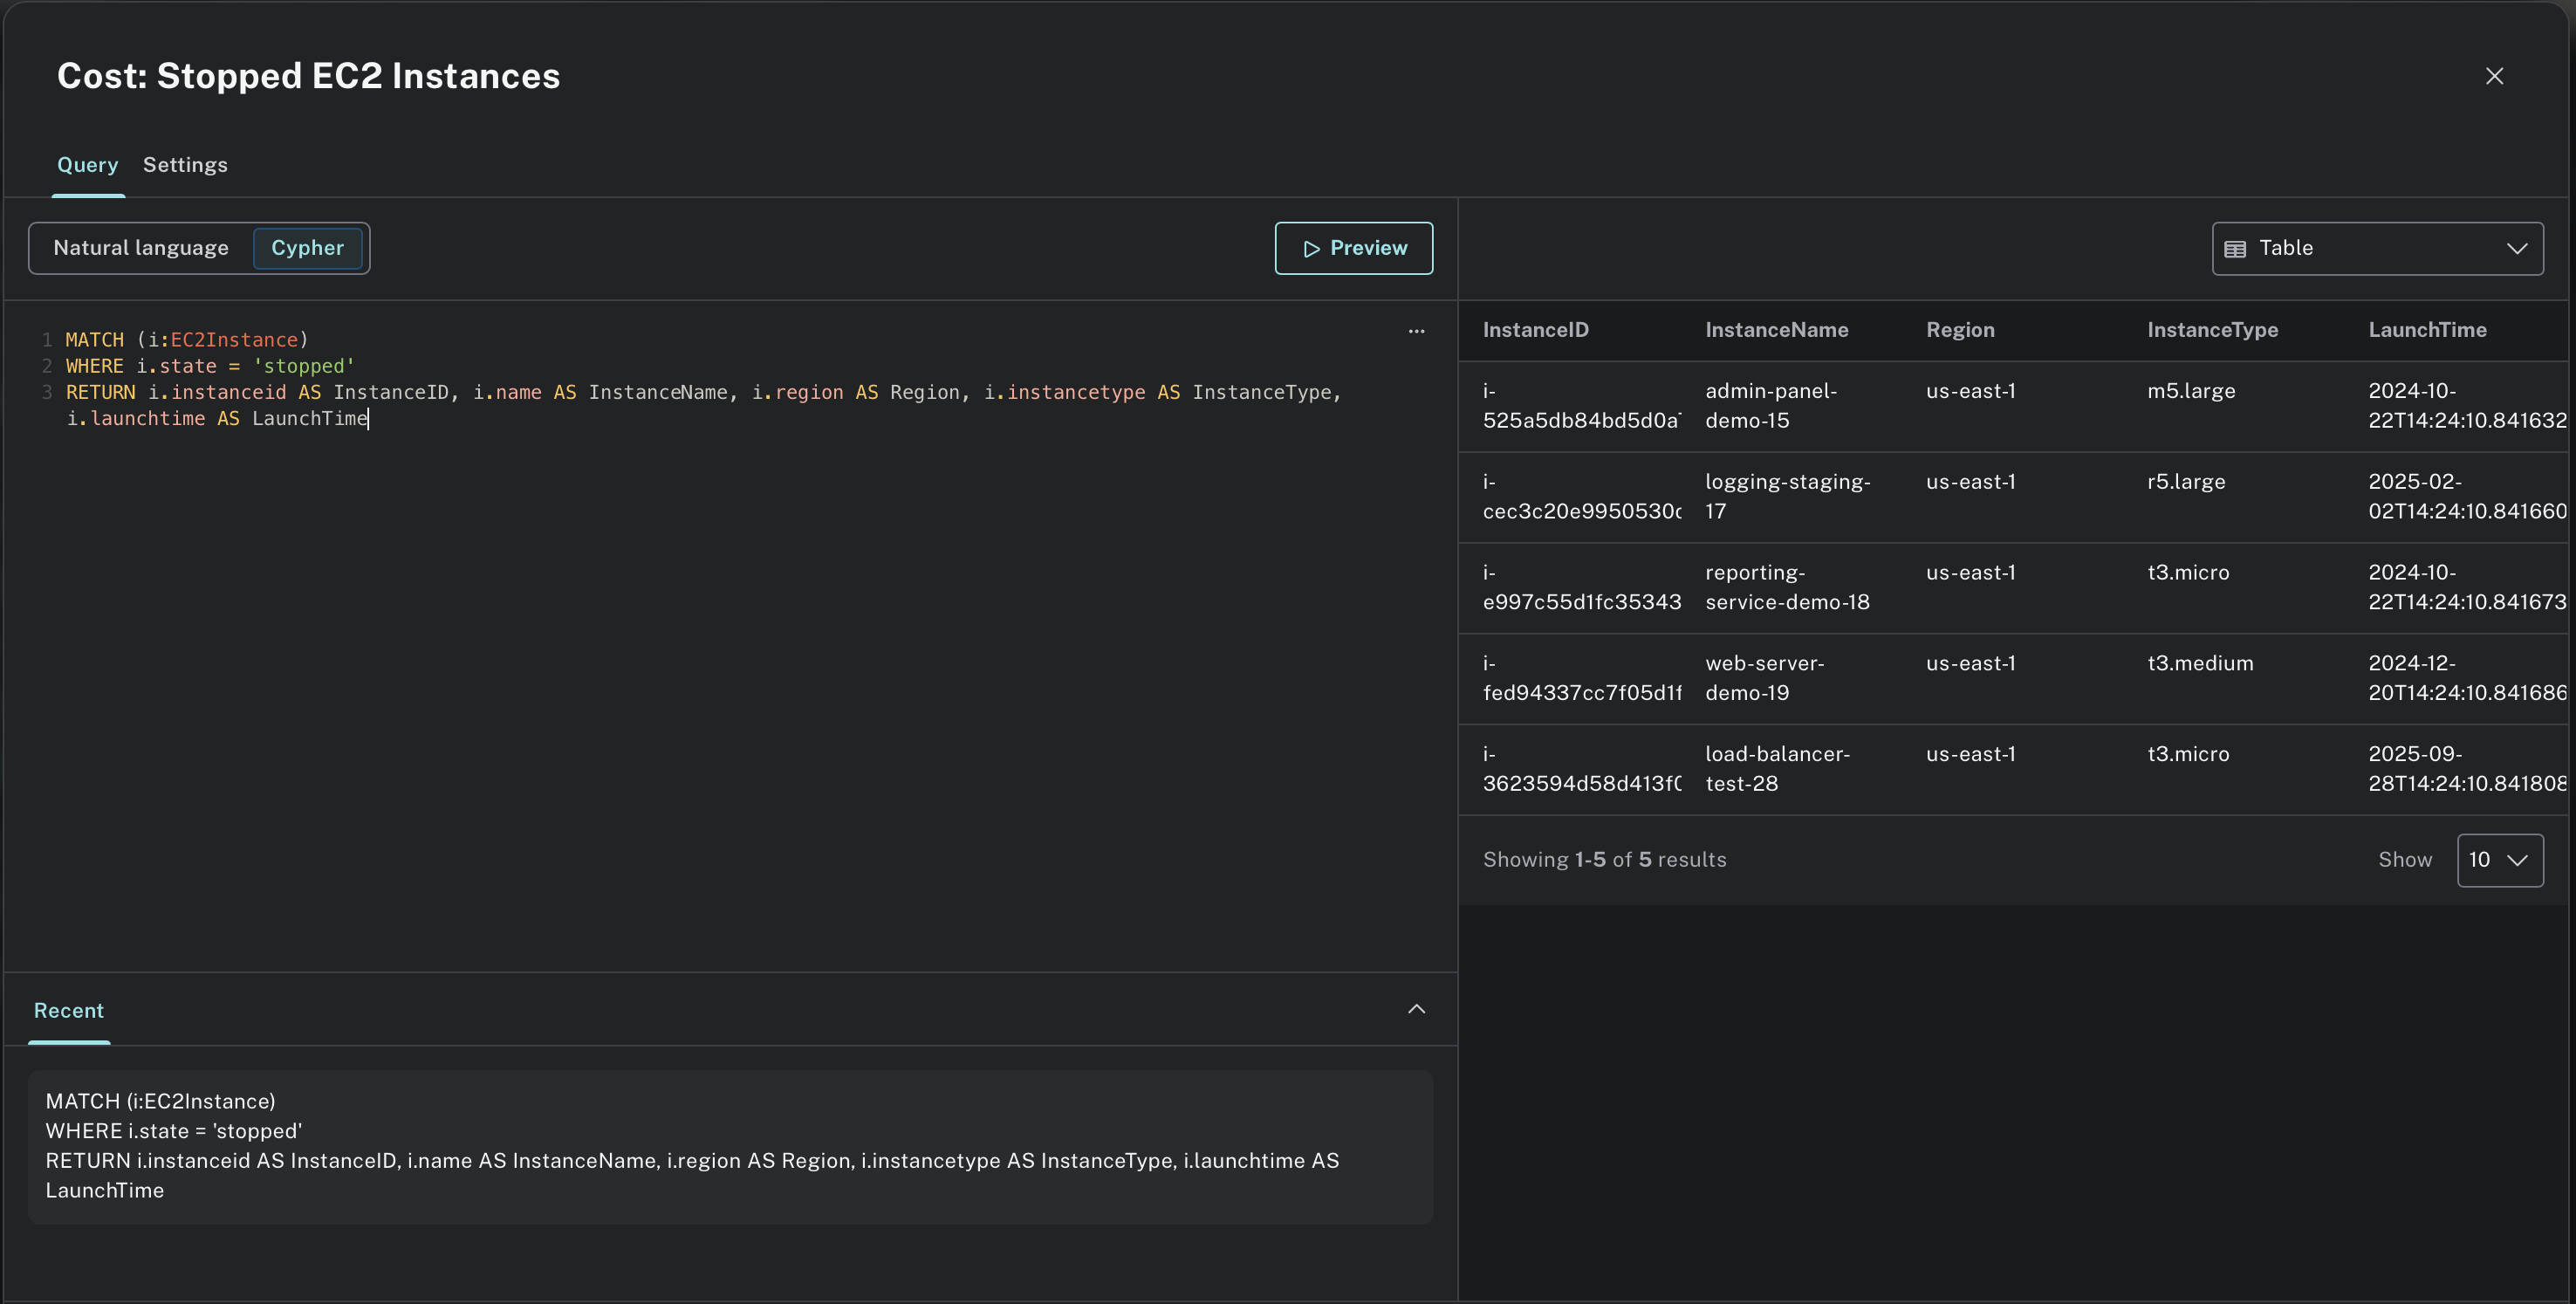
\includegraphics[width=0.8\textwidth]{Stopped EC2 Instances.png}
\caption{已停止的 EC2 實例檢測}
\label{fig:stopped_ec2}
\end{figure}

\subsubsection{故障衝擊分析查詢結果}

\begin{figure}[H]
\centering
\begin{subfigure}[b]{0.48\textwidth}
\centering
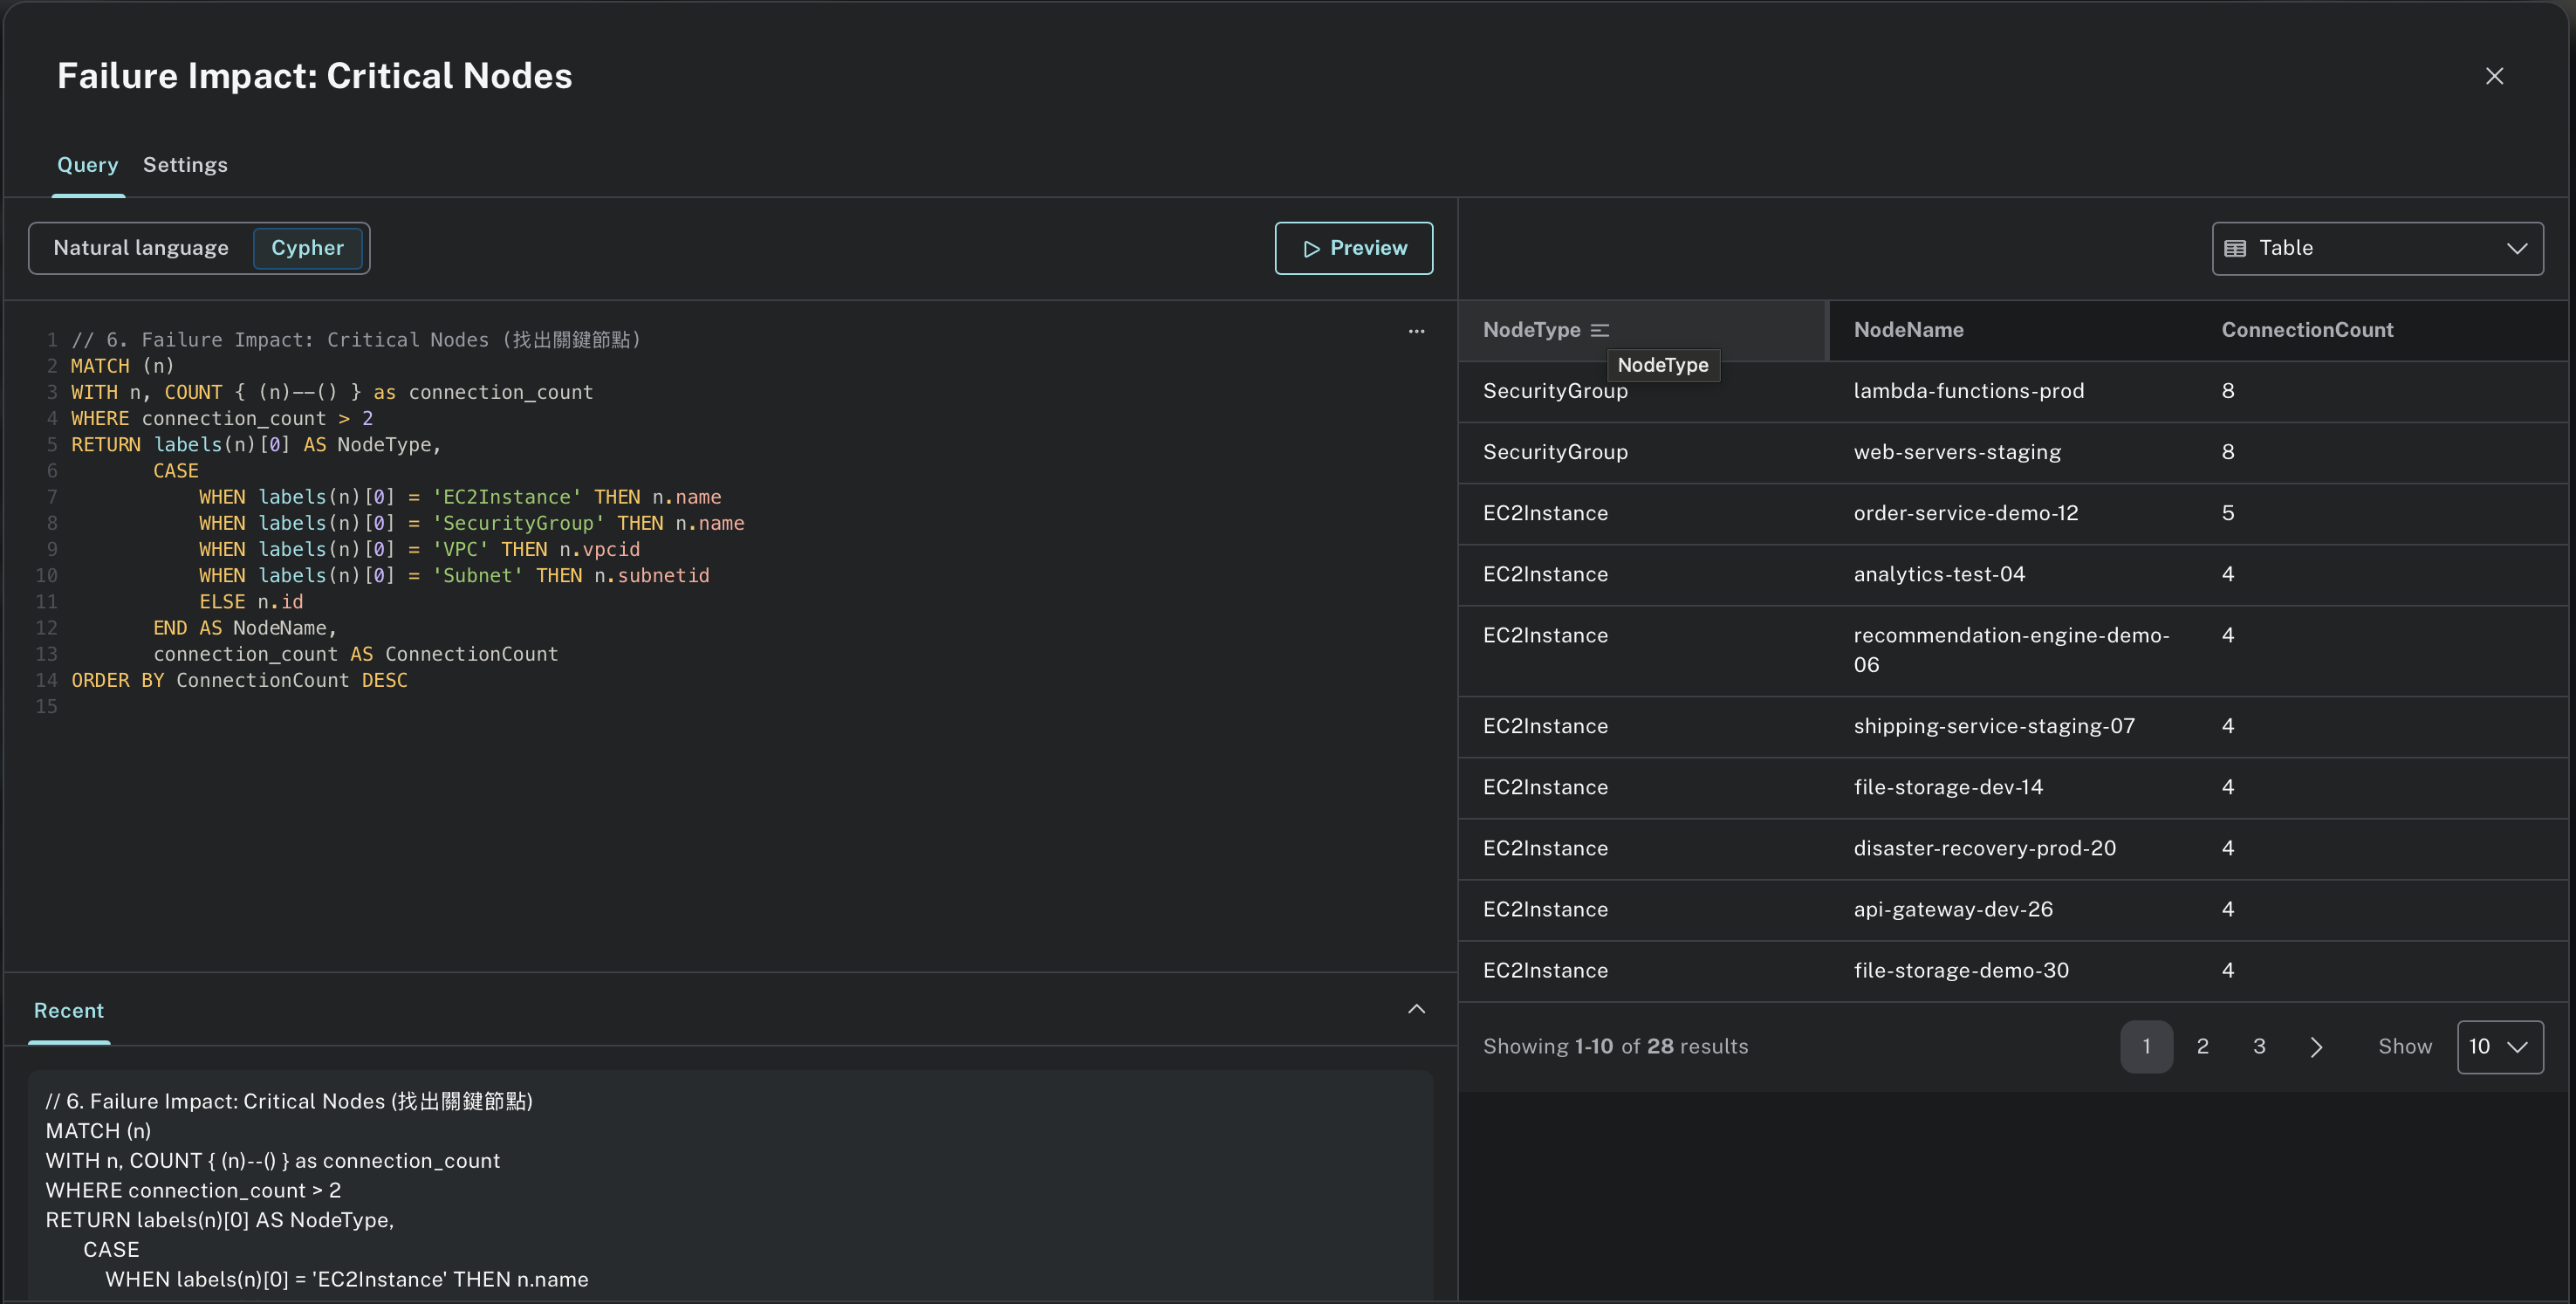
\includegraphics[width=\textwidth]{Critical Nodes.png}
\caption{關鍵節點識別}
\label{fig:critical_nodes}
\end{subfigure}
\hfill
\begin{subfigure}[b]{0.48\textwidth}
\centering
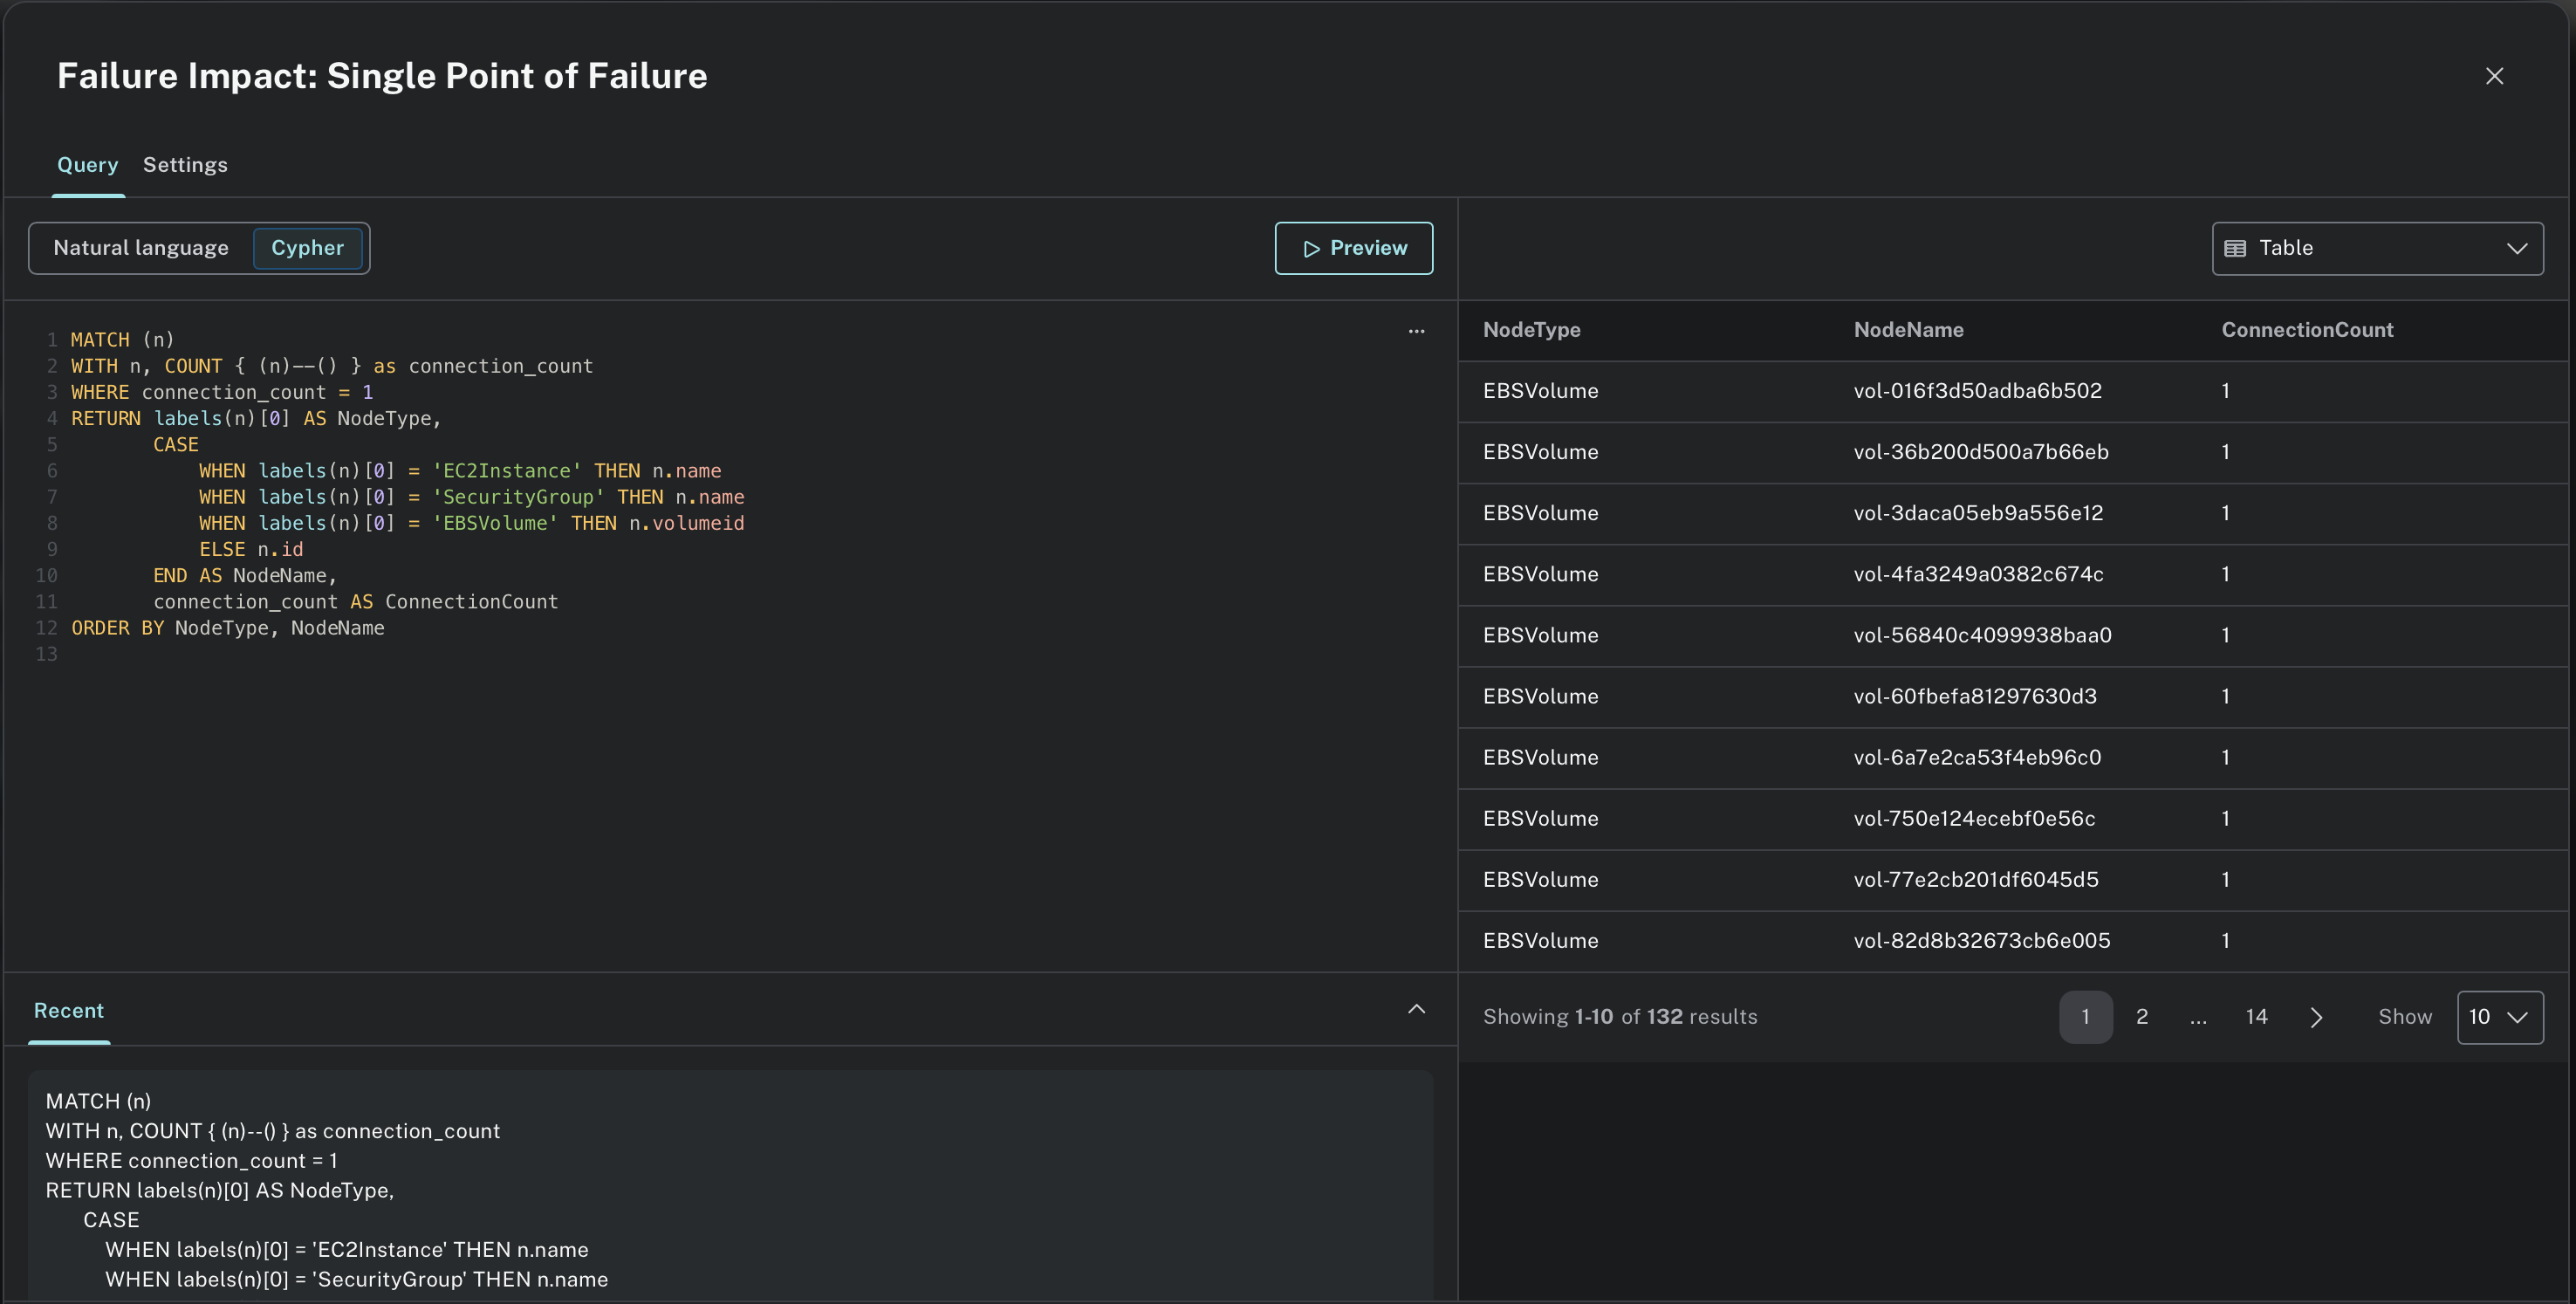
\includegraphics[width=\textwidth]{Single Point of Failure.png}
\caption{單點故障檢測}
\label{fig:spof}
\end{subfigure}
\caption{故障衝擊分析查詢結果}
\label{fig:failure_analysis_results}
\end{figure}

\begin{figure}[H]
\centering
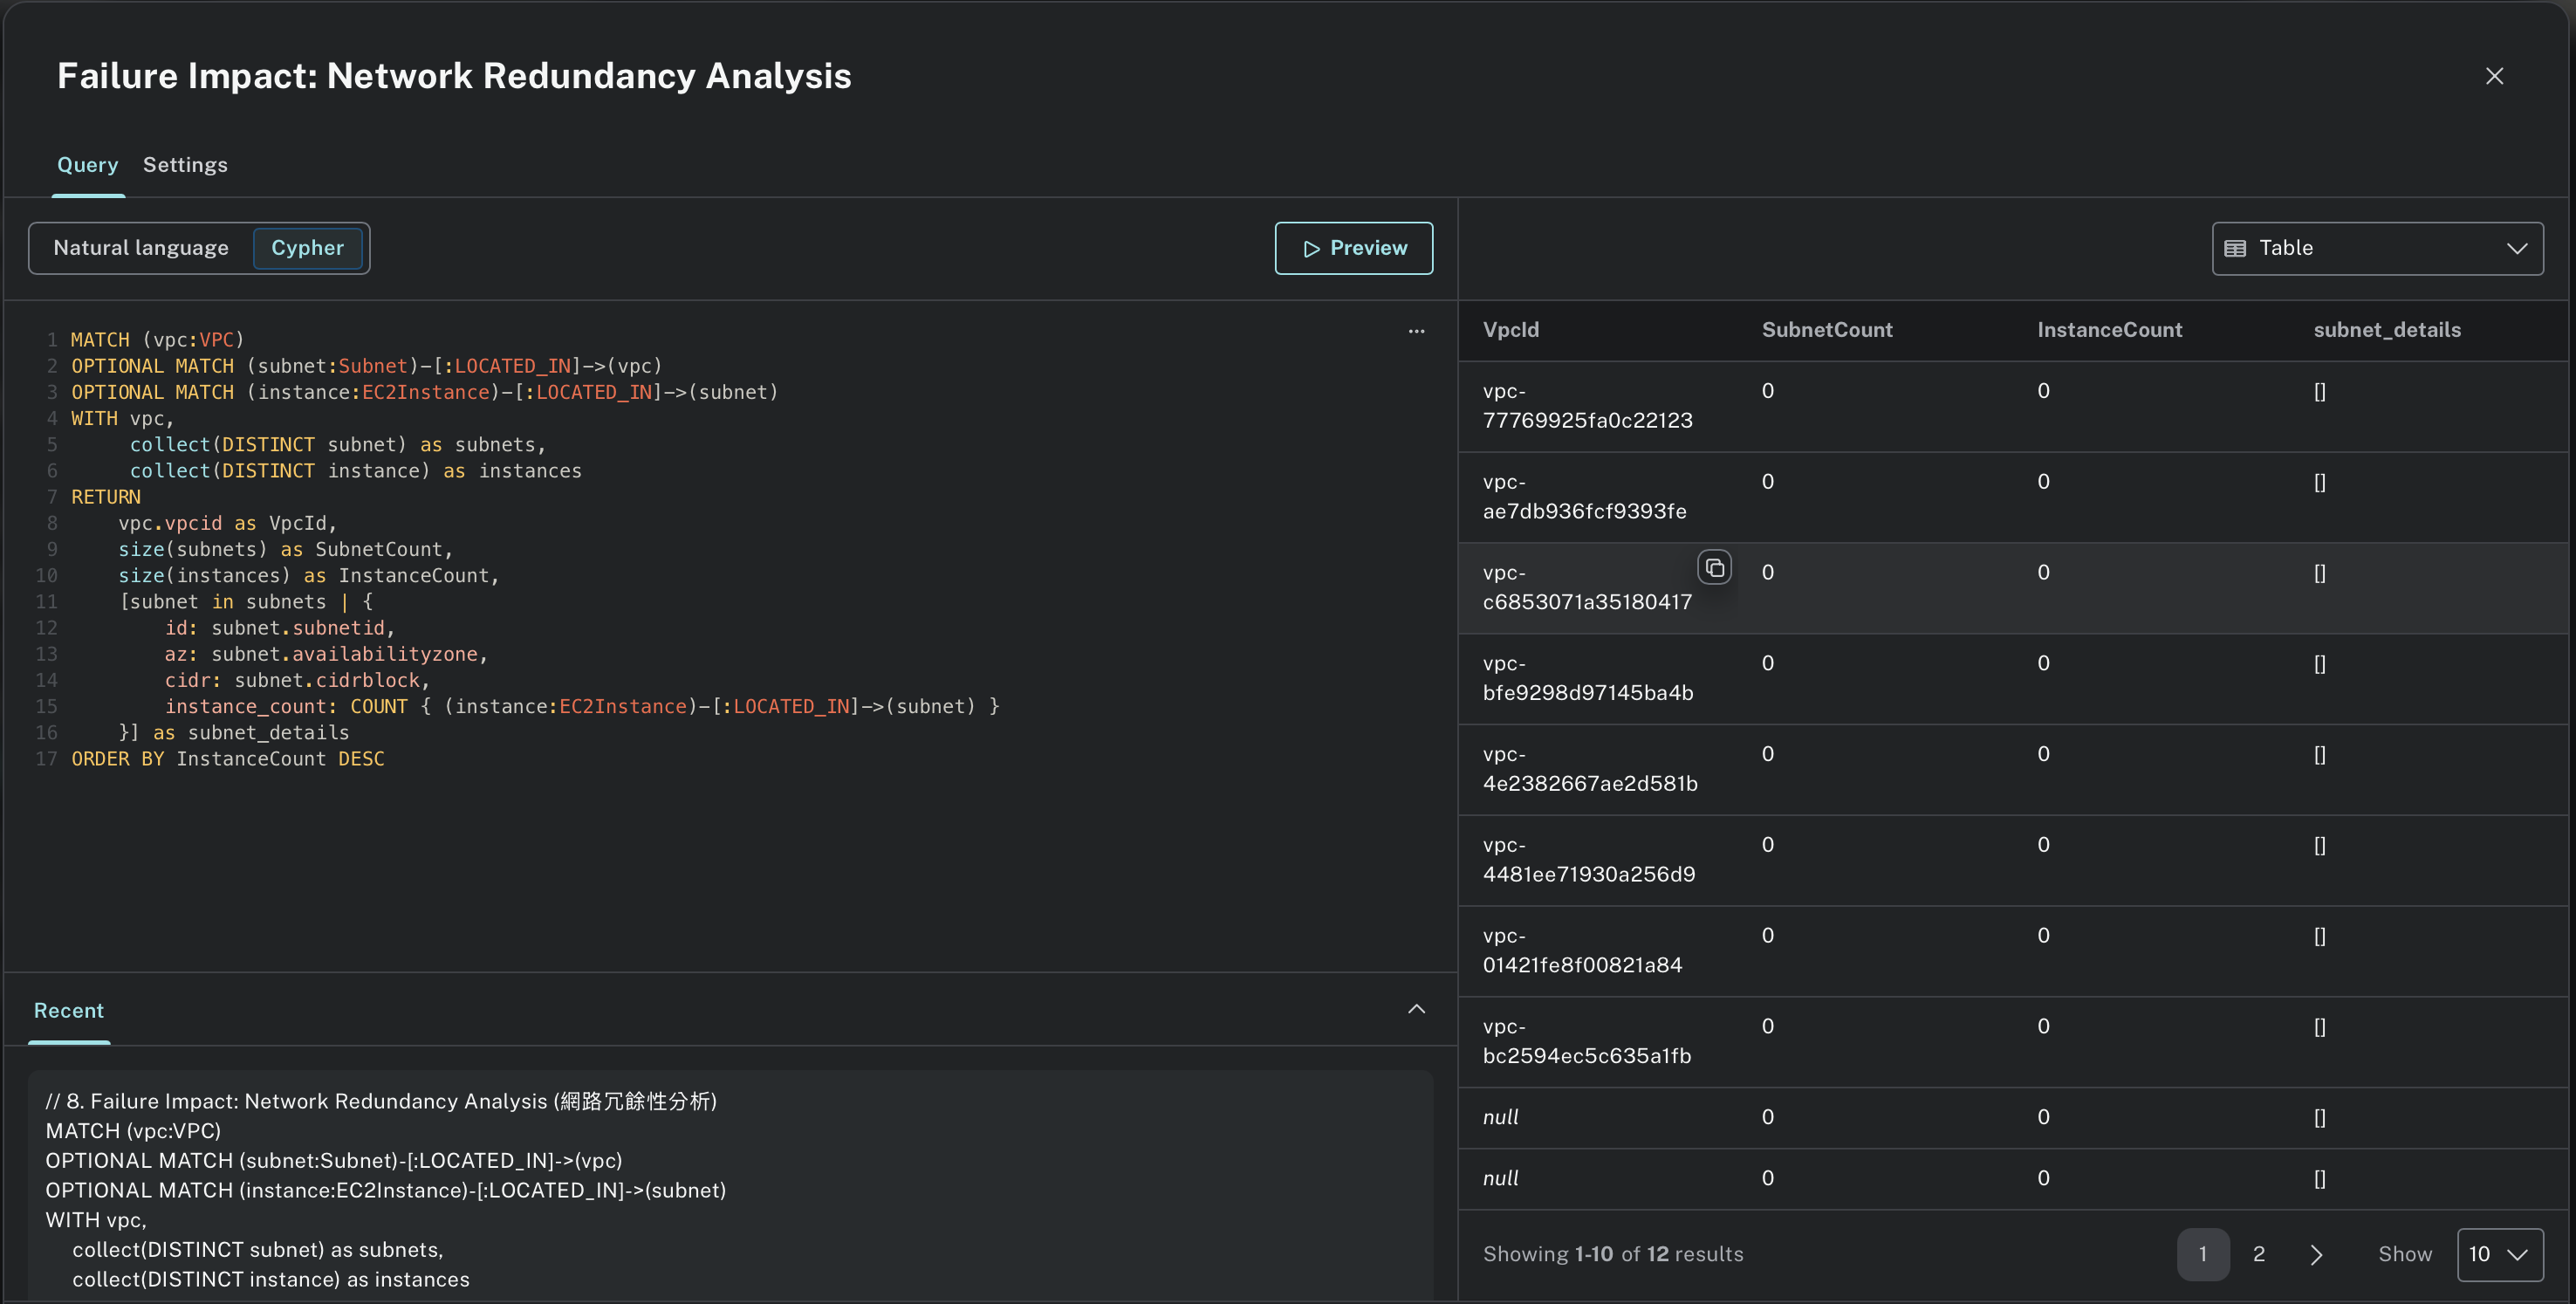
\includegraphics[width=0.8\textwidth]{Network Redundancy Analysis.png}
\caption{網路冗餘性分析}
\label{fig:network_redundancy}
\end{figure}

\section{參考資料}

\begin{enumerate}[leftmargin=1.5em]
\item Neo4j Documentation: https://neo4j.com/docs/
\item Cypher Query Language: https://neo4j.com/docs/cypher-manual/
\item AWS Well-Architected Framework: https://aws.amazon.com/architecture/well-architected/
\item Cartography Project: https://github.com/lyft/cartography
\item 專案 GitHub 儲存庫: https://github.com/itsYoga/cloud-infra-analysis
\end{enumerate}

---
\end{document}